% PROOF OF CONCEPT
Next, the potential and the difficulties of the theory presented in the preceding section are investigated.
The goal is to give a proof of concept for the basic feasibility of spectral Bayesian inference.
It is verified that the theory can be successfully applied in practice and further insight into its functioning is obtained.
Moreover, it is learned about its current shortcomings.
Four instructive calibration problems from classical statistics and inverse modeling are solved for these purposes.
The analysis is confined to problems with low-dimensional parameter spaces.
First, the mean value of a normal distribution is inferred with random data under a conjugate normal prior.
Second, the mean and standard deviation of a normal distribution are fitted for a joint prior with independent and uniform marginals.
Third, an inverse heat conduction problem in two spatial dimensions with two unknowns is solved.
Finally, a similar thermal problem with six unknowns is considered.
Synthetically created pseudo-data are used in all these example applications.
\par % CONVERGENCE BEHAVIOR
As it turns out, one can gain valuable insights into the characteristics of likelihood expansions and posterior emulators by way of comparison.
Therefore, the analyses for the first three examples proceed analogously.
For rich experimental designs, the convergence behavior of high-degree SLEs is studied by reference to the LOO error.
More importantly, the capability of lower-degree SLEs to accurately capture the posterior QoI-expectations is explored for scarcer experimental designs.
Eventually, aSLE-based posterior surrogates are investigated in order to mitigate the curse of dimensionality.
All results are compared to reference solutions.
Where possible, the exact solutions from a conjugate Bayesian analysis are used to this effect.
Otherwise, corresponding approximations are computed via classical MCMC sampling.
\par % UQLAB
The uncertainty quantification platform UQLab \cite{Computing:Marelli2014:Proc,Computing:Uqlab2015:Manual09104} is used throughout the numerical demonstrations.
It provides a flexible environment for the uncertainty analysis of engineering systems, e.g.\ for uncertainty propagation.
In this context it ships with a range of regression tools that allow one to easily compute PCEs.
These tools can be directly applied to the likelihood function in order to compute SLEs.
OLS is employed as the standard solving routine in the following examples.

\subsection{1D normal fitting}
% GAUSSIAN FITTING
First of all, we consider the problem of fitting a Gaussian distribution \(\mathcal{N}(y_i \cond \mu,\sigma^2)\) to random realizations \(y_i\) with \(i = 1,\ldots,\dimData\).
The goal is to estimate the unknown mean \(\mu\) whereas the standard deviation \(\sigma\) is assumed to be already known.
Given a Gaussian prior, this one-dimensional normal model with known variance exhibits a Gaussian posterior density.
Moreover, a closed-form expression for the model evidence can be derived.
Since this offers the possibility of comparing the SLE results with analytical solutions, this simple statistical model is used as a first SLE testbed.
Let the data \(\bm{y} = (y_1,\ldots,y_\dimData)^\top\) be comprised of \(\dimData\) independent samples from the normal distribution.
For the observational model one may then write
\begin{equation} \label{eq:JCP:Conjugate:Data}
  \bm{Y} \cond \mu \sim \prod\limits_{i=1}^\dimData \mathcal{N}(y_i \cond \mu,\sigma^2), \quad \text{with known} \;\, \sigma^2.
\end{equation}
% POSTERIOR DISTRIBUTION
Consequently, the likelihood function can be simply written as \(\mathcal{L}(\mu) = \prod_{i=1}^{\dimData} \mathcal{N}(y_i \cond \mu,\sigma^2)\).
A Bayesian prior distribution \(\pi(\mu)\) captures the epistemic uncertainty of the true value of \(\mu\) before the data analysis.
For the posterior distribution, that aggregates the information about the unknown after the data have been analyzed, one then has \(\pi(\mu \cond \bm{y}) = \scale^{-1} \mathcal{L}(\mu) \pi(\mu)\).
\par % CONJUGATE ANALYSIS
The conjugate prior for the data model in \cref{eq:JCP:Conjugate:Data} is a Gaussian \(\pi(\mu) = \mathcal{N}(\mu \cond \mu_0,\sigma_0^2)\).
Its mean \(\mu_0 = \mathds{E}[\mu]\) and variance \(\sigma_0^2 = \mathrm{Var}[\mu]\) have to be conveniently specified by the experimenter and data analyst.
This prior choice ensures that the posterior is a Gaussian \(\pi(\mu \cond \bm{y}) = \mathcal{N}(\mu \cond \mu_\dimData,\sigma_\dimData^2)\)
whose parameters \(\mu_\dimData = \mathds{E}[\mu \cond \bm{y}]\) and \(\sigma_\dimData^2 = \mathrm{Var}[\mu \cond \bm{y}]\) are easily found as
\begin{equation} \label{eq:JCP:Conjugate:Posterior}
  \mu_\dimData = \left( \frac{1}{\sigma_0^2} + \frac{\dimData}{\sigma^2} \right)^{-1} \left( \frac{\mu_0}{\sigma_0^2} + \frac{\dimData \overline{y}}{\sigma^2} \right),
  \quad \sigma_\dimData^2 = \left( \frac{1}{\sigma_0^2} + \frac{\dimData}{\sigma^2} \right)^{-1}.
\end{equation}
Here, \(\overline{y} = N^{-1} \sum_{i=1}^N y_i\) is the empirical sample mean of the data.
% MODEL EVIDENCE
Likewise, an explicit expression for the model evidence
\(\scale = \int_{\mathds{R}} (\prod_{i=1}^\dimData \mathcal{N}(y_i \cond \mu, \sigma^2)) \, \mathcal{N}(\mu \cond \mu_0,\sigma_0^2) \, \mathrm{d} \mu\) can be derived.
Let \(\overline{y^2} = N^{-1} \sum_{i=1}^N y_i^2\) denote the sample mean of the squared observations.
A straightforward calculation based on simple algebra and a Gaussian integral then yields
\begin{equation} \label{eq:JCP:Conjugate:ModelEvidence}
  \scale = \sigma_0^{-1} \left( \sigma \sqrt{2 \pi} \right)^{-\dimData} \left( \frac{1}{\sigma_0^2} + \frac{\dimData}{\sigma^2} \right)^{-1/2}
  \exp \left( - \frac{1}{2} \left( \frac{\mu_0^2}{\sigma_0^2} + \frac{\dimData \overline{y^2}}{\sigma^2}
  - \left( \frac{1}{\sigma_0^2} + \frac{\dimData}{\sigma^2} \right)^{-1} \left( \frac{\mu_0}{\sigma_0^2} + \frac{\dimData \overline{y}}{\sigma^2} \right)^2 \right) \right).
\end{equation}
\par % EXPERIMENTAL SETUP
For the following computer experiment, the parameters of the data distribution in \cref{eq:JCP:Conjugate:Data} are specified as \(\mu = 10\) and \(\sigma = 5\), respectively.
In the course of the procedure only the mean is treated as an unknown, whereas the standard deviation is assumed to be known.
We consider a situation where \(\dimData = 10\) samples are randomly drawn from the data distribution.
For the numerical experiment, the pseudo-random numbers \(\bm{y} = (8.78,4.05,12.58,3.60,11.05,8.70,20.80,1.23,19.36,12.07)^\top\) are used as synthetic data.
The prior distribution is set to be a Gaussian \(\pi(\mu) = \mathcal{N}(\mu \cond \mu_0,\sigma_0^2)\) with \(\mu_0 = 11.5\) and \(\sigma_0 = 1.5\).

\subsubsection{Posterior density}
% LIKELIHOOD EXPANSION
In order to better understand the principles of spectral Bayesian inference we now proceed as follows.
Spectral expansions \(\hat{\mathcal{L}}_p\) of the likelihood function \(\mathcal{L}\) defined above are computed and compared
for experimental designs of varying size \(K\) and polynomial terms of varying degree \(p\).
Hermite polynomials are used in combination with an appropriate linear transformation to standardized variables
\(\xi_\mu \in \mathds{R}\) with a Gaussian weight function \(\mathcal{N}(\xi_\mu \cond 0,1)\).
Accordingly, the unknown can be represented as \(\mu = \mu_0 + \sigma_0 \xi_\mu\).
The experimental designs are one-dimensional Sobol sequences that are appropriately transformed.
\par % SLE CONVERGENCE
First the convergence behavior and the accuracy of the likelihood approximation are analyzed.
For a rich experimental design with \(K = 5 \times 10^4\), SLEs are computed for an increasing order up to \(p = 20\).
The normalized empirical error \(\epsilon_{\mathrm{Emp}}\) and the normalized LOO error \(\epsilon_{\mathrm{LOO}}\) are monitored over these computations.
While the former can be directly computed according to its definition, the computation of the latter relies on the reformulation in \cref{eq:JCP:PCE:SimpleLOO}.
This serves the purpose of assessing the prediction accuracy of the computed SLE as a function of the degree \(p\).
The results are plotted in \cref{fig:JCP:Conjugate:ConvSLE}.
It can be seen how the error estimates approach zero, i.e.\ the SLE converges to the likelihood function.
For \(p = 20\) the empirical error amounts to \(\epsilon_{\mathrm{Emp}} = 1.05 \times 10^{-12}\) and the LOO amounts to \(\epsilon_{\mathrm{LOO}} = 1.82 \times 10^{-10}\).
These small error magnitudes show that the likelihood function \(\mathcal{L}\) can be indeed spectrally expanded in a Hermite basis.
% FIGURE: SLE CONVERGENCE
\begin{figure}[htbp]
  \centering
  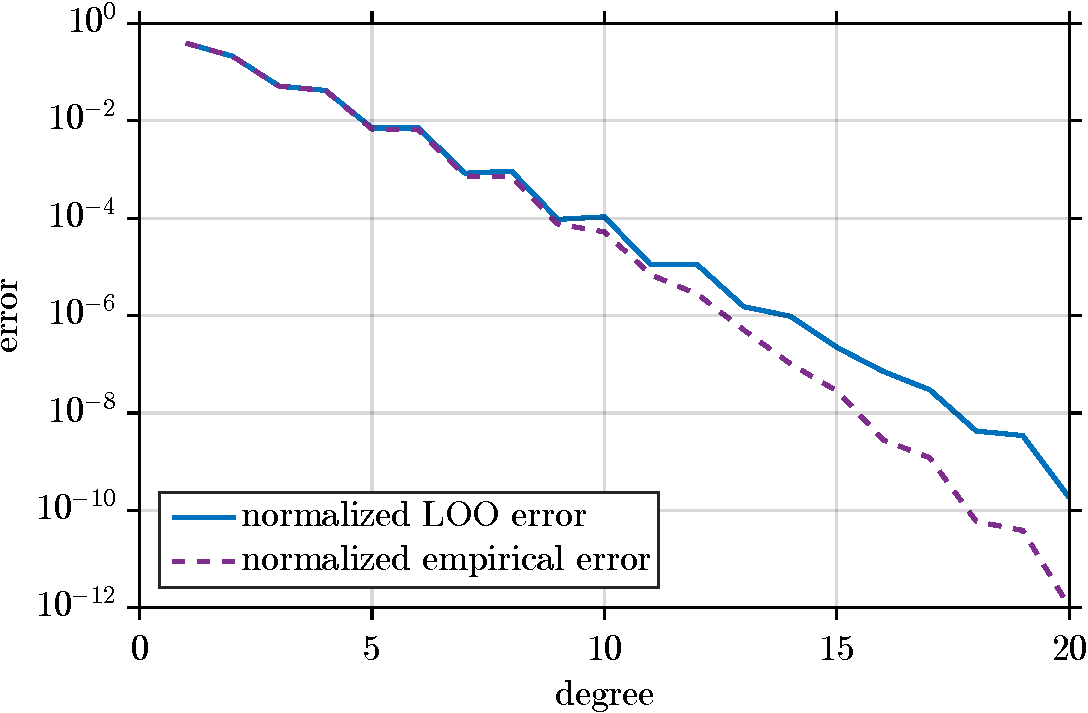
\includegraphics[height=\JCPfigHeight]{fig_JCP_Norm1D_ConvSLE}
  \caption[1D normal fitting: Convergence of the SLE]{1D normal fitting: Convergence of the SLE.}
  \label{fig:JCP:Conjugate:ConvSLE}
\end{figure}
\par % LIKELIHOOD FUNCTION
The functional likelihood approximation \(\hat{\mathcal{L}}_p\) provided by the most accurate SLE with \(p = 20\) is visualized in \cref{fig:JCP:Conjugate:Like}.
Moreover, the plot shows a low-order SLE with \(p = 5\) and \(K = 1 \times 10^2\) for which the error estimates
\(\epsilon_{\mathrm{Emp}} = 2.61 \times 10^{-4}\) and \(\epsilon_{\mathrm{LOO}} = 8.41 \times 10^{-4}\) are obtained.
For the sake of comparison the exact likelihood function \(\mathcal{L}\) is shown as well.
It can be seen that the SLEs are able to accurately represent the likelihood around its peak,
i.e.\ roughly speaking in the interval \(\mu \in [8,15]\) for \(p = 5\) and in \(\mu \in [5,18]\) for \(p = 20\).
Note that these regions accumulate the largest proportions of the total prior probability mass.
Outside of these ranges, however, the SLEs \(\hat{\mathcal{L}}_p\) start strongly deviating from \(\mathcal{L}\) and taking on negative values.
These phenomena can be attributed to an imperfect polynomial cancellation of the finite series approximation of the likelihood
in the regions of the parameter space that are only sparsely covered by the experimental design.
Indeed, for unbounded parameter spaces it is clearly hopeless to achieve a global net cancellation of a finite polynomial expansion
that is necessary in order to emulate the vanishing behavior of the likelihood far from its peaks.
The extent to which this impacts on the approximation of the posterior density and its first moments is investigated next.
\par % POSTERIOR DENSITY
Expanding the likelihood function is only a means to the end of surrogating the posterior density.
Approximations of the posterior density \(\pi(\mu \cond \bm{y}) \approx \coeffL_0^{-1} \hat{\mathcal{L}}_p(\mu) \pi(\mu)\)
are computed from the SLEs with \(p = 5\) and \(p = 20\) through \cref{eq:JCP:SLE:Posterior,eq:JCP:SLE:ScaleFactor}.
The results are plotted in \cref{fig:JCP:Conjugate:Post}.
In addition to the SLE approximations, the prior density \(\pi(\mu) = \mathcal{N}(\mu \cond \mu_0,\sigma_0^2)\) and the exact solution
\(\pi(\mu \cond \bm{y}) = \mathcal{N}(\mu \cond \mu_\dimData,\sigma_\dimData^2)\) from a conjugate analysis based on \cref{eq:JCP:Conjugate:Posterior} are shown.
The posterior surrogate for \(p = 5\) shows minor deviations from the the analytical result,
while the approximation for \(p = 20\) perfectly matches the true density.
% EXPONENTIAL DECAY
It is noted that the discrepancies between \(\hat{\mathcal{L}}_p\) and \(\mathcal{L}\) shown in \cref{fig:JCP:Conjugate:Like} are attenuated.
The underlying reason is that for large enough \(\lvert \mu \rvert \rightarrow \infty\) the exponential decay of the Gaussian prior \(\pi(\mu) \propto \exp(-(\mu-\mu_0)^2)\)
dominates the polynomial increase of \(\hat{\mathcal{L}}_p(\mu) = \sum_{\alpha=0}^p \coeffL_{\alpha} \basis_{\alpha}(\mu)\) in the sense that \(\hat{\mathcal{L}}_p(\mu) \pi(\mu) \rightarrow 0\).
This absorbs the effects of the SLE approximation that is increasingly inadequate for large values of \(\lvert \mu \rvert\).
In this sense, the prior reference density guards the posterior surrogate against the inadequacies of the SLE.
Therefore, the posterior emulation may very well be more accurate than the SLE approximation of the likelihood.
% FIGURES: LIKELIHOOD & POSTERIOR
\begin{figure}[htbp]
  \begin{minipage}[b]{\JCPsubWidth}
    \centering
    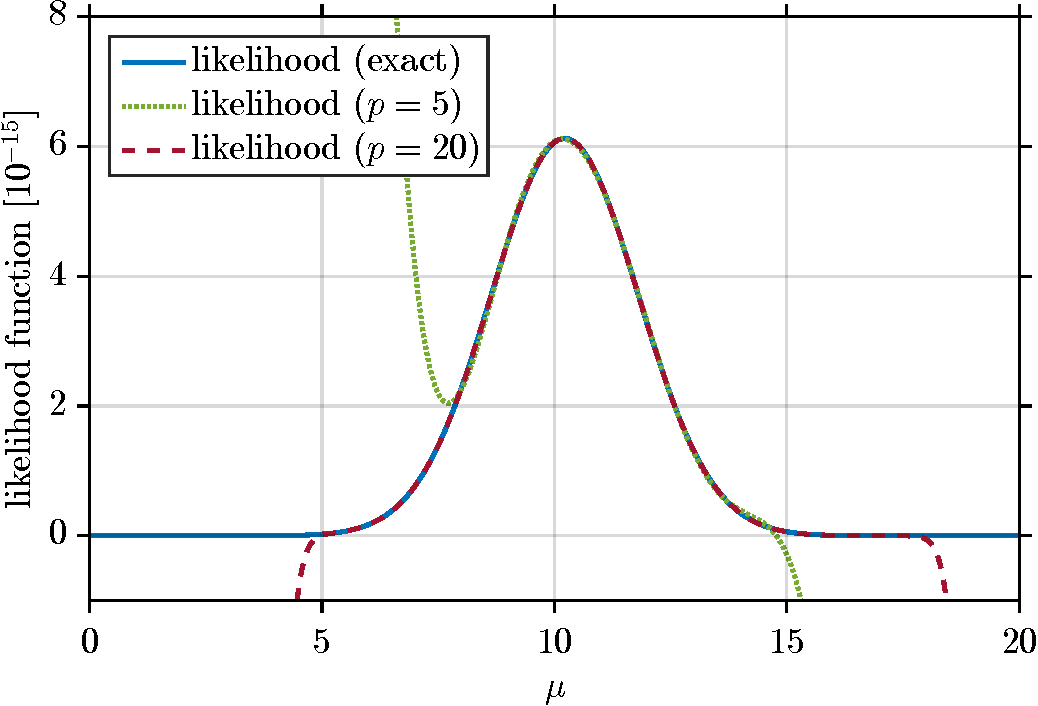
\includegraphics[height=\JCPfigHeight]{fig_JCP_Norm1D_Like}
    \caption[1D normal fitting: Likelihood function]{1D normal fitting: Likelihood function.}
    \label{fig:JCP:Conjugate:Like}
  \end{minipage}%
  \hfill%
  \begin{minipage}[b]{\JCPsubWidth}
    \centering
    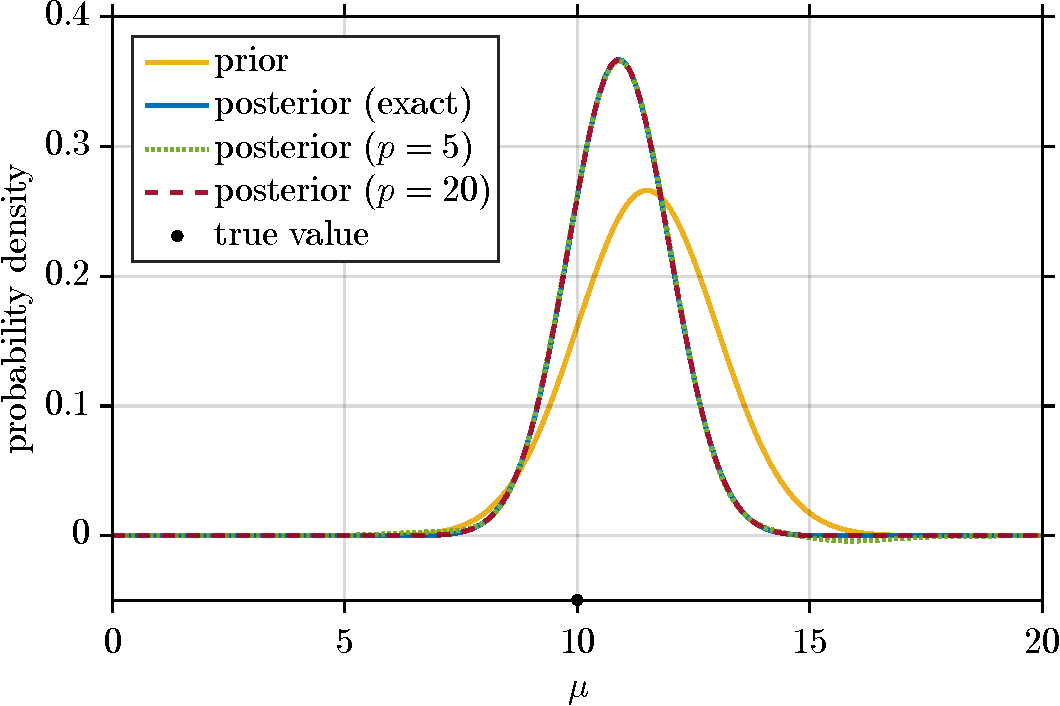
\includegraphics[height=\JCPfigHeight]{fig_JCP_Norm1D_Post}
    \caption[1D normal fitting: Posterior density]{1D normal fitting: Posterior density.}
    \label{fig:JCP:Conjugate:Post}
  \end{minipage}%
\end{figure}

\subsubsection{Quantities of interest}
% STATISTICAL QUANTITIES OF INTEREST
Commonly one employs posterior means as parameter estimates and posterior standard deviations as measures of the estimation uncertainty.
In order to investigate how well one can approximate the model evidence together with these meaningful quantities in spectral Bayesian inference,
SLEs are computed for experimental designs of varying size \(K\) and for a selection of expansion orders \(p\).
The corresponding SLE-based approximations of the model evidence \(\scale\), the posterior mean \(\mu_\dimData\) and the standard deviation \(\sigma_\dimData\)
are then computed from \cref{eq:JCP:SLE:ScaleFactor,eq:JCP:SLE:PosteriorMargMean,eq:JCP:SLE:PosteriorMargVariance}.
Note that the effects of the transformation to standard variables have to be appropriately taken care of at this place.
This happens via \cref{eq:JCP:PCE:IntegrationBySubstitution}.
The SLE approximations can then be compared to the analytical solutions that are obtained from the conjugate analysis in \cref{eq:JCP:Conjugate:Posterior,eq:JCP:Conjugate:ModelEvidence}.
In \cref{tab:JCP:Conjugate:StatisticalQuantities} the results of this procedure are summarized.
Note that all the SLE estimates attain admissible values, e.g.\ the model evidence is non-negative.
Furthermore, it is noticed that \(\scale\), \(\mu_\dimData\) and \(\sigma_\dimData\) can be recovered with high accuracy even for very scarce experimental designs and low-order SLEs,
say for \(K = 1 \times 10^3\) and \(p = 10\).
It is concluded that, in some sense, the accurate estimation of the model evidence and the first posterior moments
require significantly less computational effort than the accurate estimation of the posterior density.
% TABLE: STATISTICAL QUANTITIES
\begin{table}[htbp]
  \caption[1D normal fitting: Statistical quantities]{1D normal fitting: Statistical quantities.}
  \label{tab:JCP:Conjugate:StatisticalQuantities}
  \centering
  \begin{tabular}{ccccccc}
    \toprule
    & \(K\) & \(p\) & \(\epsilon_{\mathrm{LOO}}\) & \(\scale\) \([10^{-15}]\) & \(\mu_\dimData\) & \(\sigma_\dimData\) \\
    \midrule
    \multirow{6}{*}{\rotatebox[origin=c]{90}{SLE}}
    & \(1 \times 10^2\) &  \(5\) & \(8.41 \times 10^{-4}\) & \(3.71\) & \(10.85\) & \(0.92\) \\
    & \(5 \times 10^2\) &  \(8\) & \(2.49 \times 10^{-4}\) & \(3.75\) & \(10.91\) & \(1.14\) \\
    & \(1 \times 10^3\) & \(10\) & \(2.58 \times 10^{-5}\) & \(3.74\) & \(10.90\) & \(1.07\) \\
    & \(5 \times 10^3\) & \(12\) & \(8.21 \times 10^{-6}\) & \(3.74\) & \(10.89\) & \(1.09\) \\
    & \(1 \times 10^4\) & \(15\) & \(3.84 \times 10^{-7}\) & \(3.74\) & \(10.89\) & \(1.09\) \\
    & \(5 \times 10^4\) & \(20\) & \(\phantom{^{1}}1.82 \times 10^{-10}\) & \(3.74\) & \(10.89\) & \(1.09\) \\
    \midrule
    \multicolumn{4}{c}{Exact results}                      & \(3.74\) & \(10.89\) & \(1.09\) \\
    \bottomrule
  \end{tabular}
\end{table}

\subsection{2D normal fitting}
% GAUSSIAN FITTING
Next, we consider the problem of fitting both the unknown mean \(\mu\) and the standard deviation \(\sigma\) of a Gaussian distribution \(\mathcal{N}(y_i \cond \mu,\sigma^2)\).
A number of independent samples \(y_i\) with \(i = 1,\ldots,\dimData\) from the normal distribution constitute the available data \(\bm{y} = (y_1,\ldots,y_\dimData)^\top\).
The data model for this situation is written as
\begin{equation} \label{eq:JCP:Normal:Data}
  \bm{Y} \cond \mu,\sigma \sim \prod\limits_{i=1}^\dimData \mathcal{N}(y_i \cond \mu,\sigma^2).
\end{equation}
% POSTERIOR DISTRIBUTION
For the likelihood function one then has \(\mathcal{L}(\mu,\sigma) = \prod_{i=1}^{\dimData} \mathcal{N}(y_i \cond \mu,\sigma^2)\).
Given a Bayesian prior \(\pi(\mu,\sigma)\), the posterior distribution is \(\pi(\mu,\sigma \cond \bm{y}) = \scale^{-1} \mathcal{L}(\mu,\sigma) \pi(\mu,\sigma)\).
This distribution aggregates the information about the two unknowns after the data have been analyzed.
\par % EXPERIMENTAL SETUP
The true values of the mean and standard deviation are set as \(\mu = 30\) and \(\sigma = 5\), respectively.
These values are treated as unknowns in the further course of the computer experiment.
We consider a situation where \(\dimData = 10\) samples are randomly drawn from the distribution in \cref{eq:JCP:Normal:Data}.
The pseudo-random numbers \(\bm{y} = (31.23,27.50,24.91,25.99,32.88,36.41,27.81,25.19,37.96,34.84)^\top\) are used as synthetic data.
We consider an independent prior \(\pi(\mu,\sigma) = \pi(\mu) \pi(\sigma)\) with uniform marginals
\(\pi(\mu) = \mathcal{U}(\mu \cond \underline{\mu},\overline{\mu})\) and \(\pi(\sigma) = \mathcal{U}(\sigma \cond \underline{\sigma},\overline{\sigma})\)
over bounded supports \(\mathcal{D}_{\mu} = [\underline{\mu},\overline{\mu}] = [20,40]\) and \(\mathcal{D}_{\sigma} = [\underline{\sigma},\overline{\sigma}] = [2,10]\).
As opposed to the conjugate example above, this two-dimensional model does not permit a closed-form expression of the posterior density and the model evidence.

\subsubsection{Posterior density}
% LIKELIHOOD EXPANSION
Now we proceed analogously to the investigation of the normal model with known variance.
Expansions \(\hat{\mathcal{L}}_p\) of the likelihood \(\mathcal{L}\) are computed and contrasted for different experimental designs of size \(K\) and different polynomial orders \(p\).
An appropriate linear transformation to uniform standardized variables is applied such that the unknowns are represented as
\(\mu = (\overline{\mu} - \underline{\mu}) / 2 \cdot \xi_{\mu} + (\underline{\mu} + \overline{\mu}) / 2\) and 
\(\sigma = (\overline{\sigma} - \underline{\sigma}) / 2 \cdot \xi_{\sigma} + (\underline{\sigma} + \overline{\sigma}) / 2\), respectively.
Here, \(\xi_{\mu},\xi_{\sigma} \in [-1,1]\) are the corresponding standardized variables with a uniform weight function.
Accordingly, tensorized Legendre polynomials form the trial basis.
Two-dimensional Sobol sequences are utilized as uniformly space-filling experimental designs.
\par % SLE CONVERGENCE
As before, the speed of convergence and the prediction accuracy of the SLE are analyzed first.
The normalized empirical error \(\epsilon_{\mathrm{Emp}}\) and the normalized LOO error \(\epsilon_{\mathrm{LOO}}\) are therefore monitored throughout a series of runs that are conducted
for an experimental design of the fixed size \(K = 1 \times 10^5\) and for an increasing expansion order up to \(p = 50\).
In \cref{fig:JCP:Normal:ConvSLE} a corresponding plot is shown, where the convergence of the SLE  \(\hat{\mathcal{L}}_p\) to the likelihood function \(\mathcal{L}\) is diagnosed.
The reason that \(\epsilon_{\mathrm{Emp}}\) and \(\epsilon_{\mathrm{LOO}}\) do not significantly differ is that the large size of the experimental design prevents overfitting.
For \(p = 50\) the normalized empirical error and the normalized LOO error are found as \(\epsilon_{\mathrm{Emp}} = 5.56 \times 10^{-11}\)
and \(\epsilon_{\mathrm{LOO}} = 6.05 \times 10^{-11}\), respectively.
This shows that the likelihood function \(\mathcal{L}\) can be indeed expanded in the Legendre basis.
For the uniform prior distribution that is used here, the normalized SLE errors effectively measure the errors of the posterior density.
% FIGURE: SLE CONVERGENCE
\begin{figure}[htbp]
  \centering
  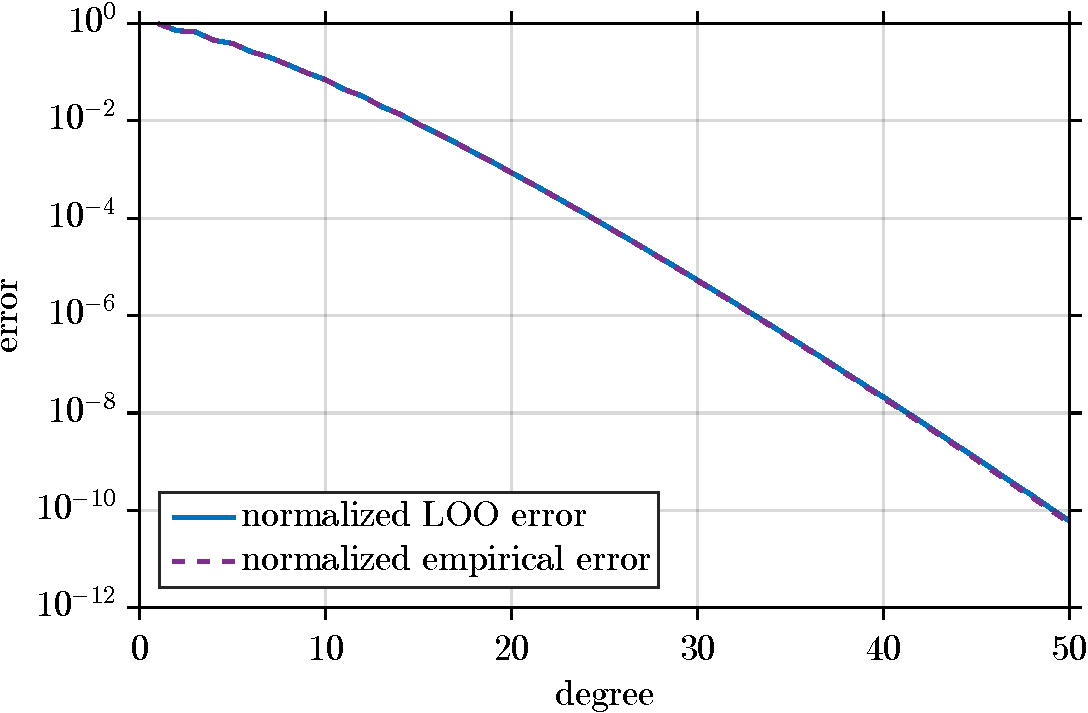
\includegraphics[height=\JCPfigHeight]{fig_JCP_Norm2D_ConvSLE}
  \caption[2D normal fitting: Convergence of the SLE]{2D normal fitting: Convergence of the SLE.}
  \label{fig:JCP:Normal:ConvSLE}
\end{figure}
\par % POSTERIOR DENSITY
Now the joint posterior density \(\pi(\mu,\sigma \cond \bm{y})\) is computed and plotted in \cref{fig:JCP:Normal:Post2D}.
For comparison purposes the posterior is sampled by means of MCMC simulation first.
A simple random walk Metropolis (RWM) sampler with a Gaussian instrumental distribution is utilized.
With this algorithm an unusually large number of \(10^7\) MCMC samples is drawn from the posterior.
This serves the purpose of providing very accurate results that act as references for the SLE-based estimates.
In \cref{fig:JCP:Normal:Post2D:MCMC} a normalized histogram of the obtained RWM sample is shown.
Next, the joint posterior density \(\pi(\mu,\sigma \cond \bm{y}) \approx \coeffL_{\bm{0}}^{-1} \hat{\mathcal{L}}_p(\mu,\sigma) \pi(\mu,\sigma)\)
is computed via \cref{eq:JCP:SLE:Posterior,eq:JCP:SLE:ScaleFactor}.
The SLE \(\hat{\mathcal{L}}_p(\mu,\sigma)\) with \(p = 50\) that features the lowest LOO error is used.
In \cref{fig:JCP:Normal:Post2D:SLE} the posterior surrogate that arises from the SLE is plotted.
For a later comparison with the heat conduction example,
in \cref{fig:JCP:Normal:Post3D:SLE} the SLE posterior surrogate from \cref{fig:JCP:Normal:Post2D:SLE} is plotted again from a different angle.
By visual inspection the obvious similarity between the density \(\pi(\mu,\sigma \cond \bm{y})\) sampled by MCMC and emulated by the SLE is noticed.
% FIGURES: 2D POSTERIORS
\begin{figure}[htbp]
  \centering
  \begin{subfigure}[b]{\JCPsubWidth}
    \centering
    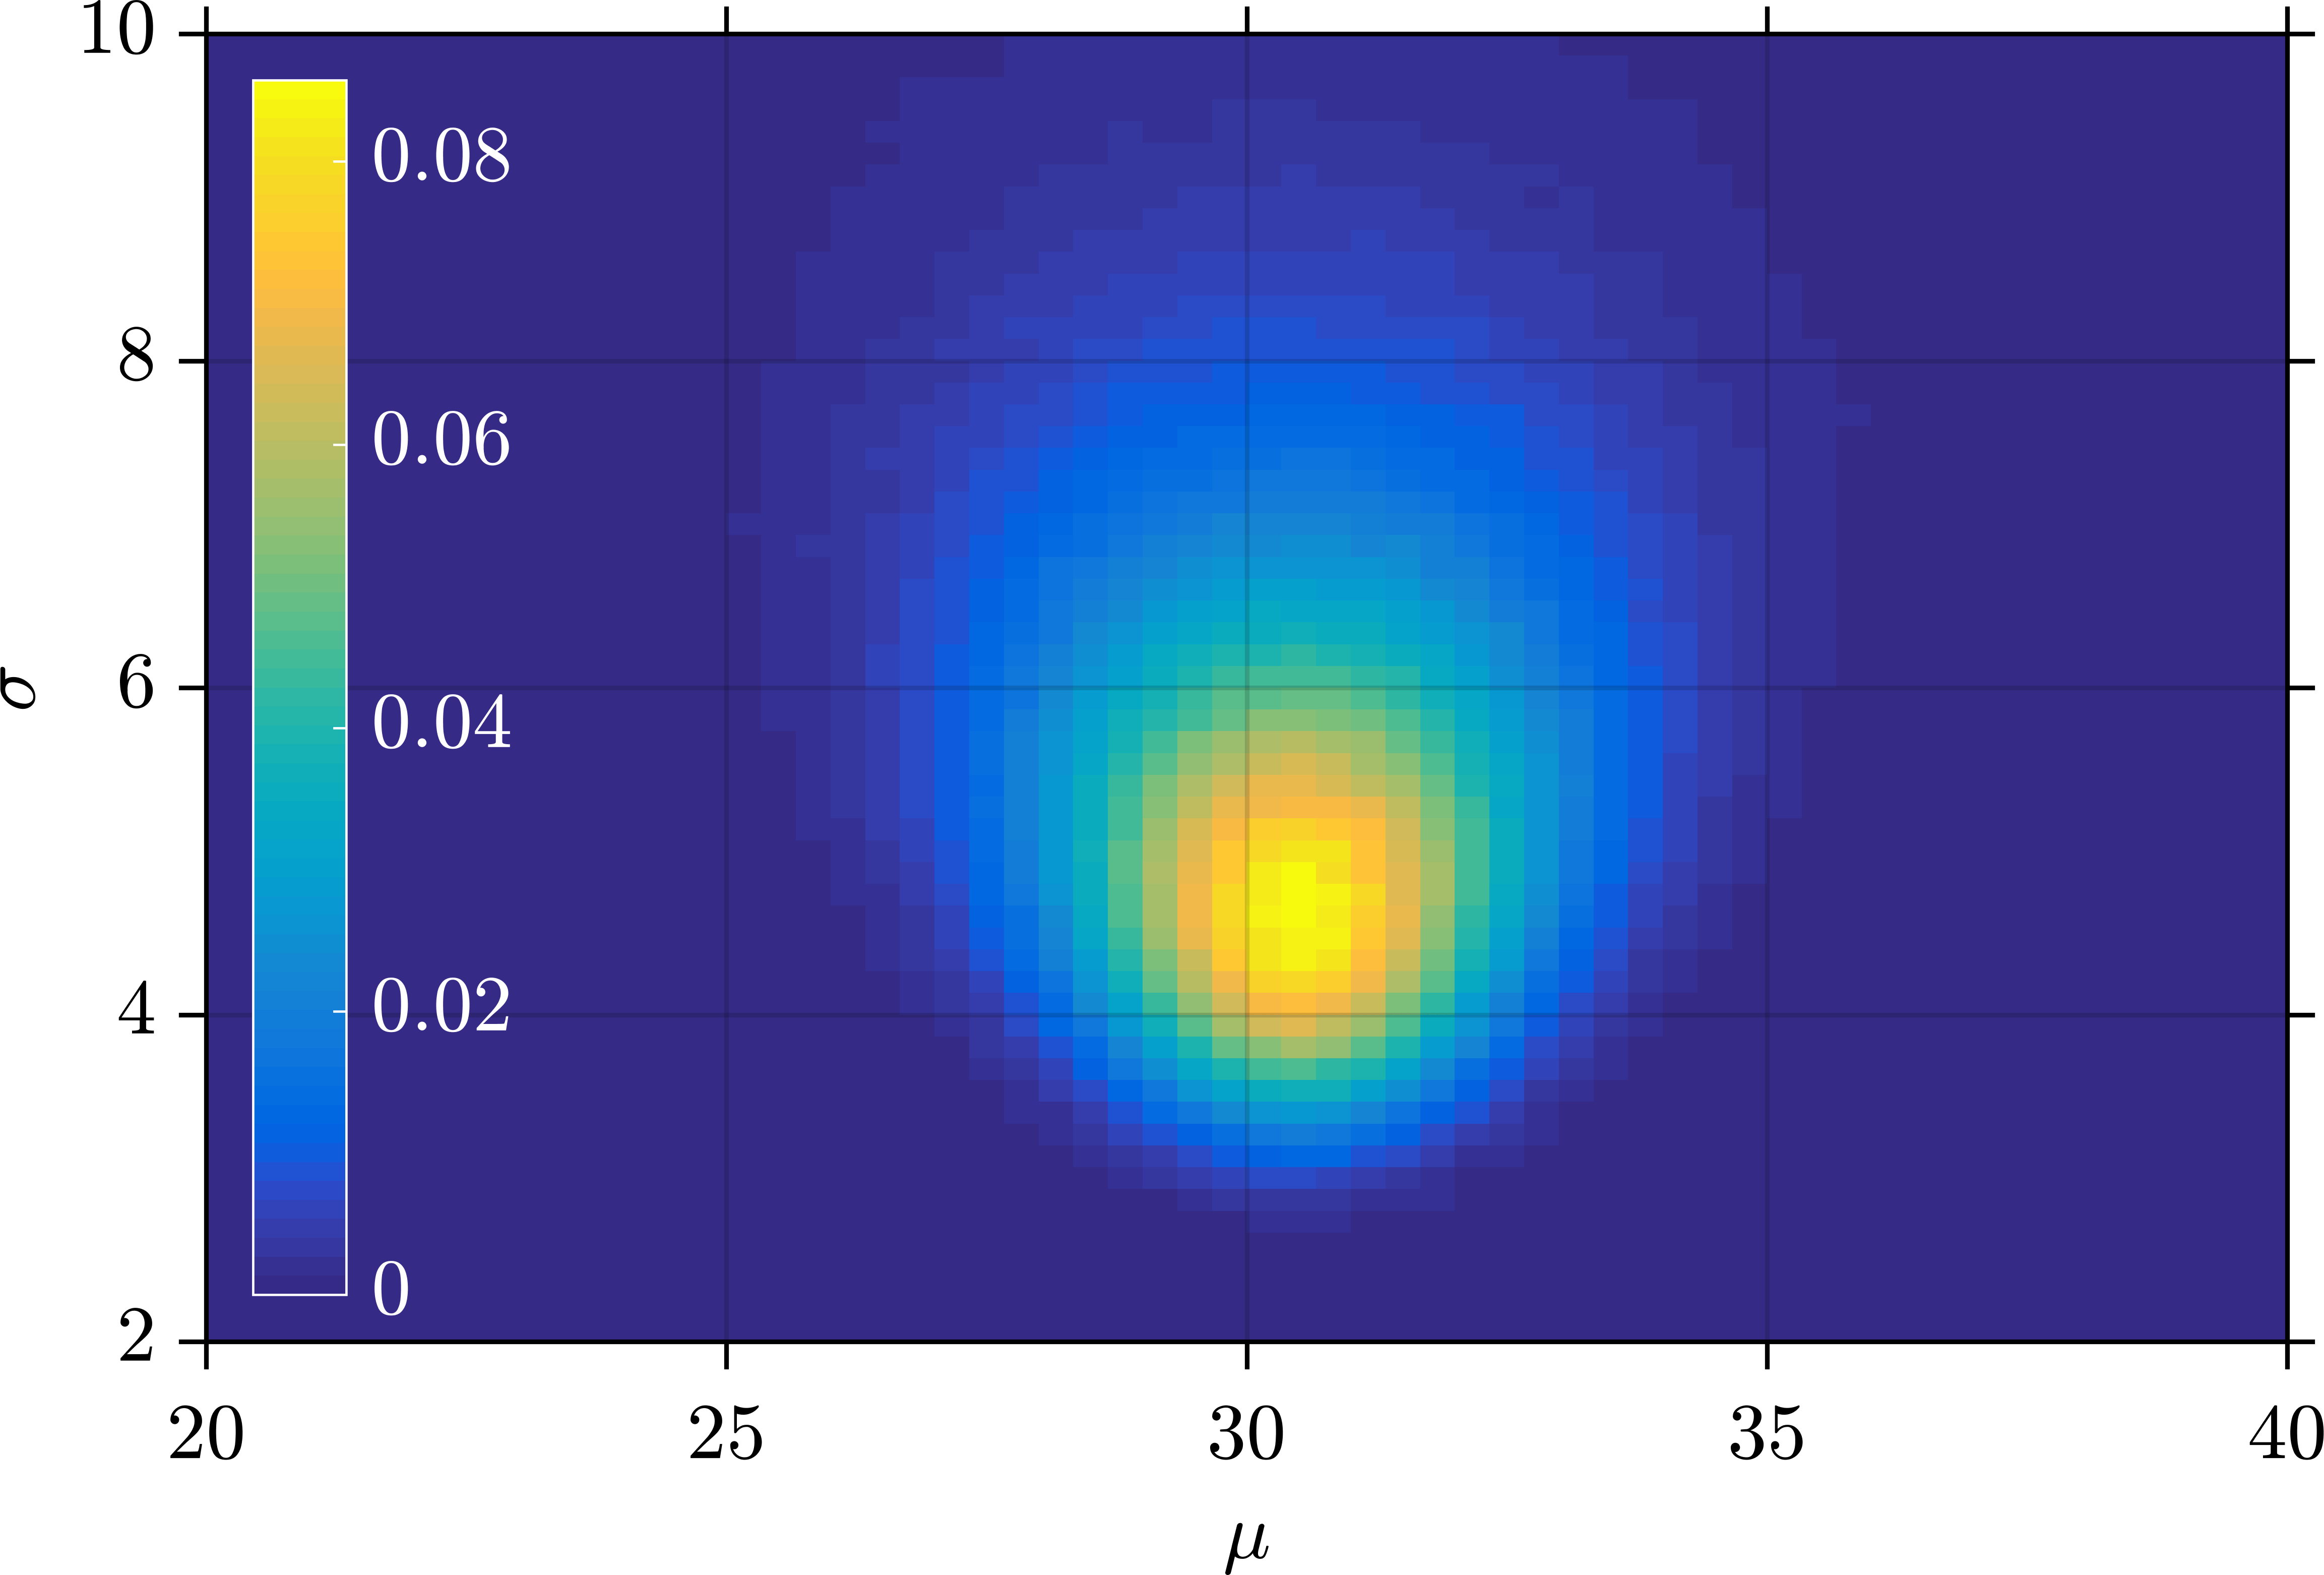
\includegraphics[height=\JCPfigHeight]{fig_JCP_Norm2D_Post2D_MCMC}
    \caption{MCMC reference sample.}
    \label{fig:JCP:Normal:Post2D:MCMC}
  \end{subfigure}\hfill%
  \begin{subfigure}[b]{\JCPsubWidth}
    \centering
    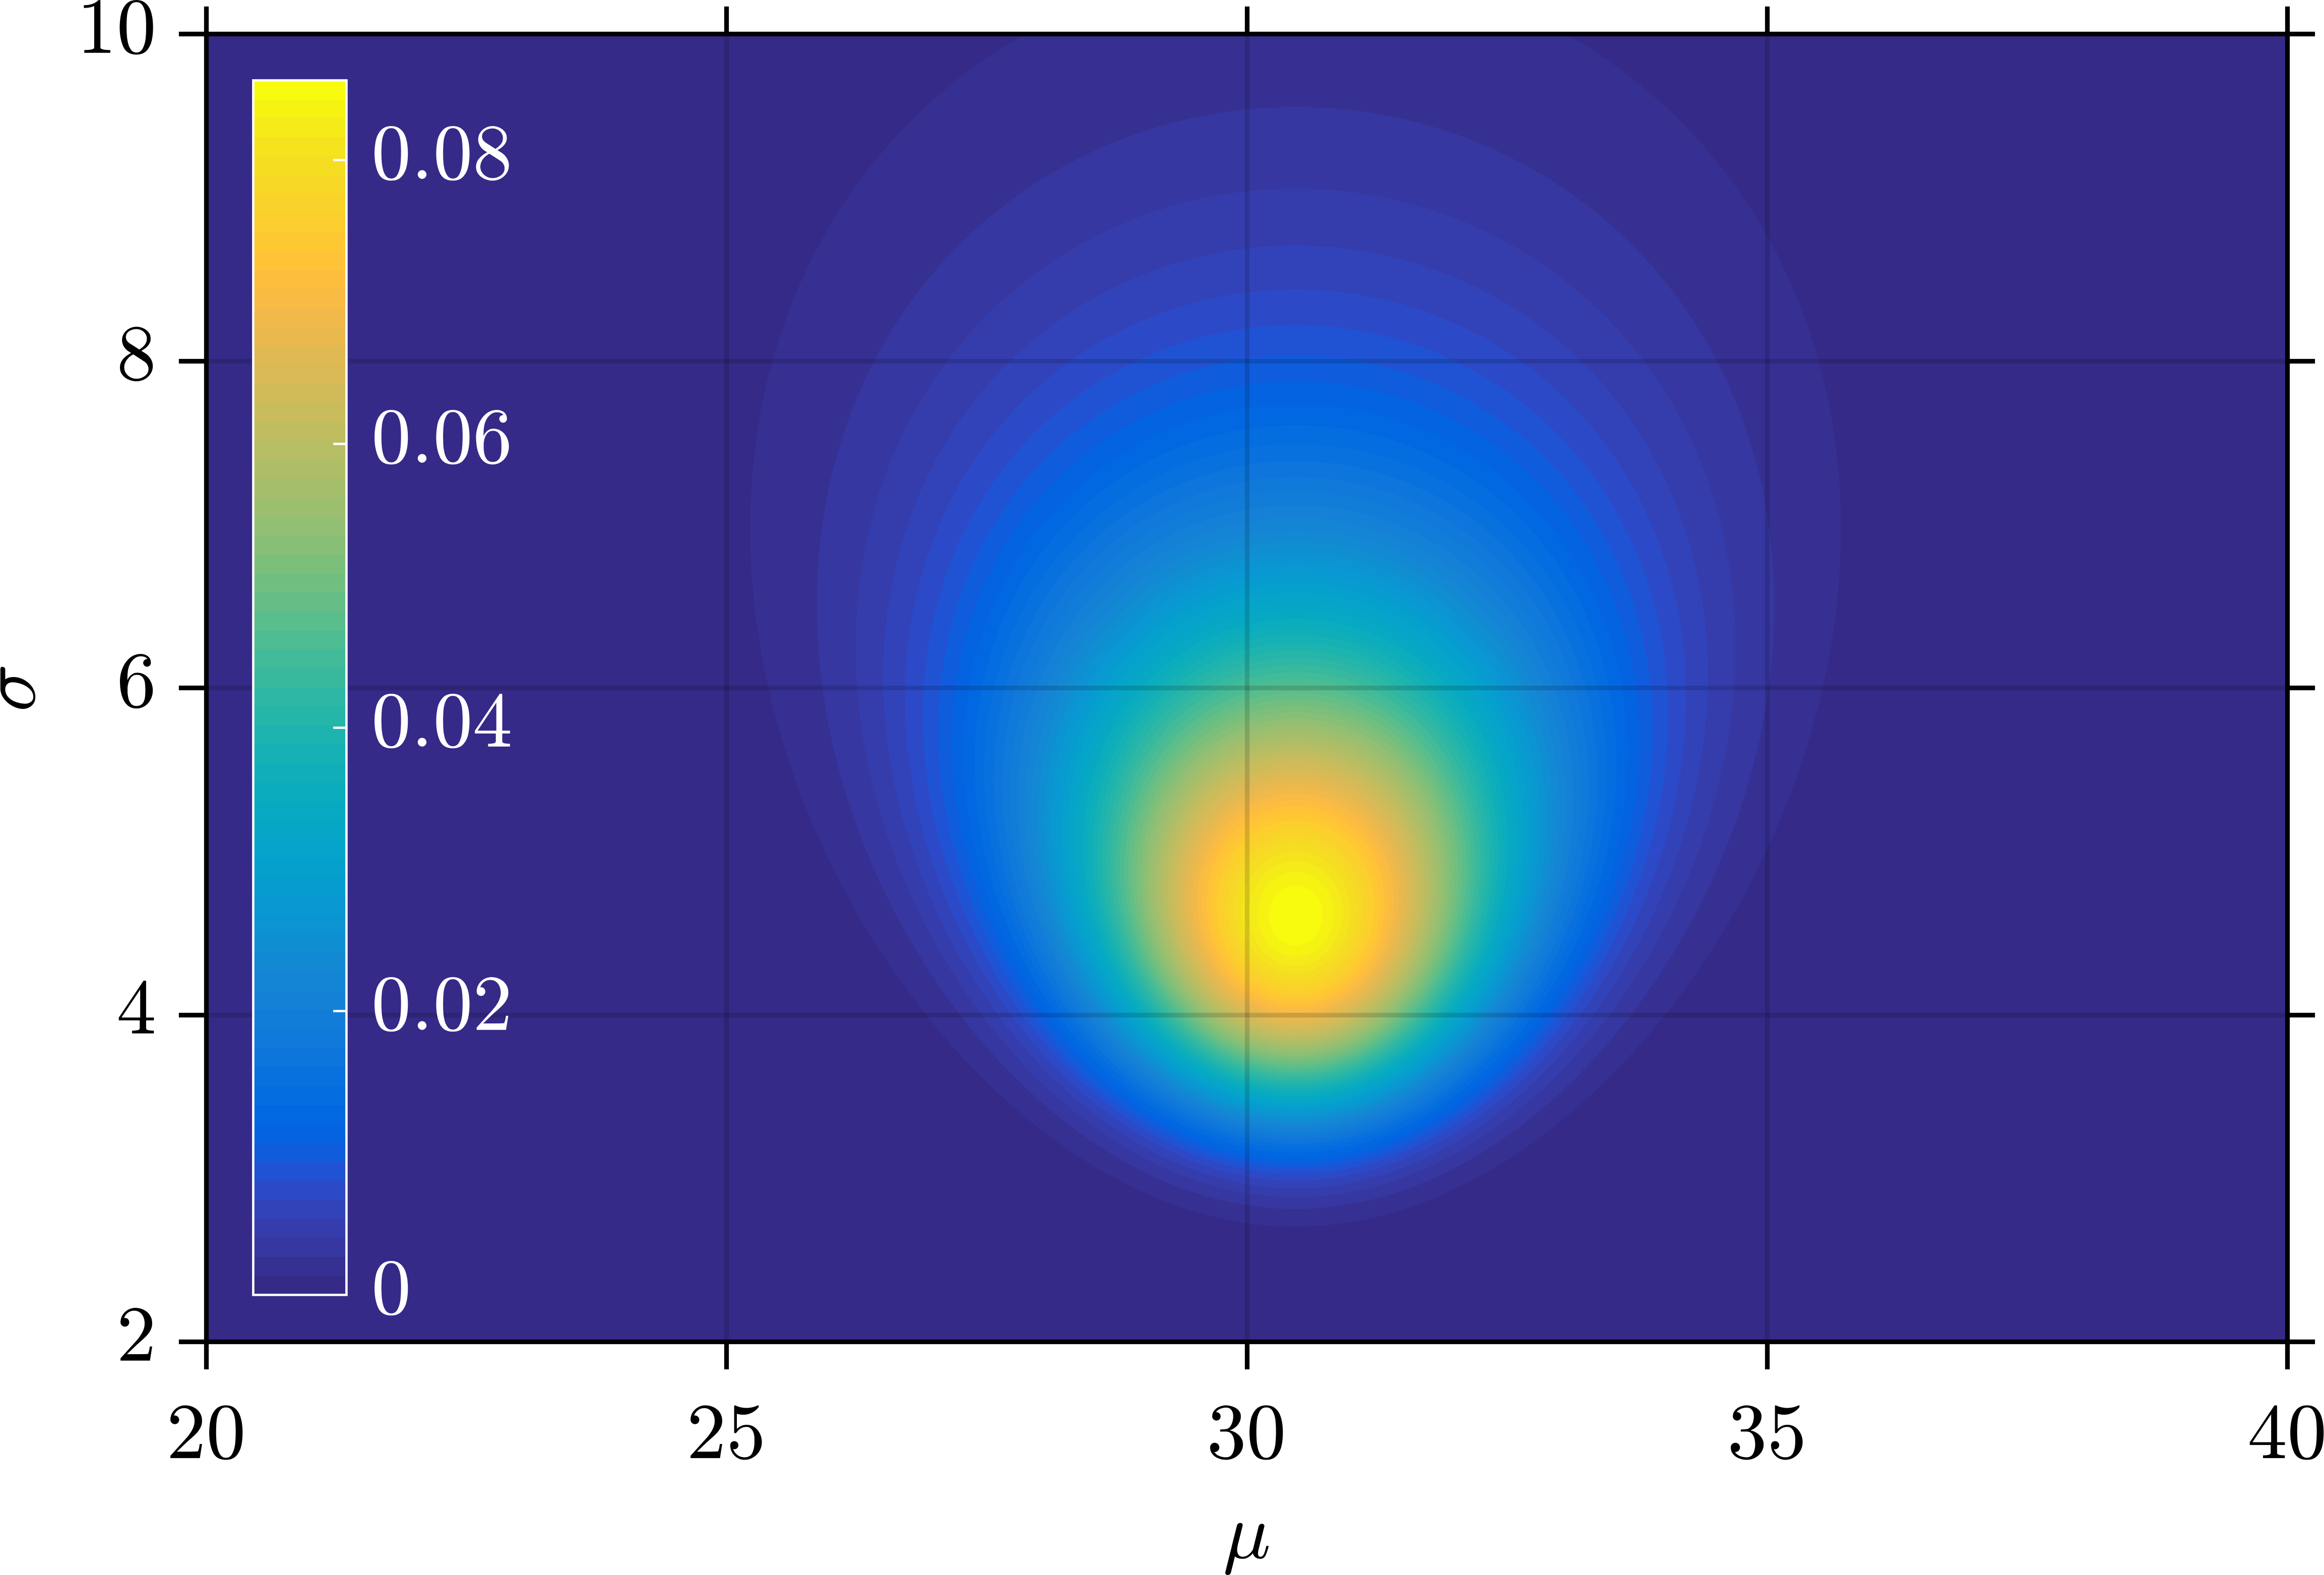
\includegraphics[height=\JCPfigHeight]{fig_JCP_Norm2D_Post2D_SLE}
    \caption{SLE with \(p = 50\).}
    \label{fig:JCP:Normal:Post2D:SLE}
  \end{subfigure}\\[1ex]%
  \begin{subfigure}[b]{\JCPsubWidth}
    \centering
    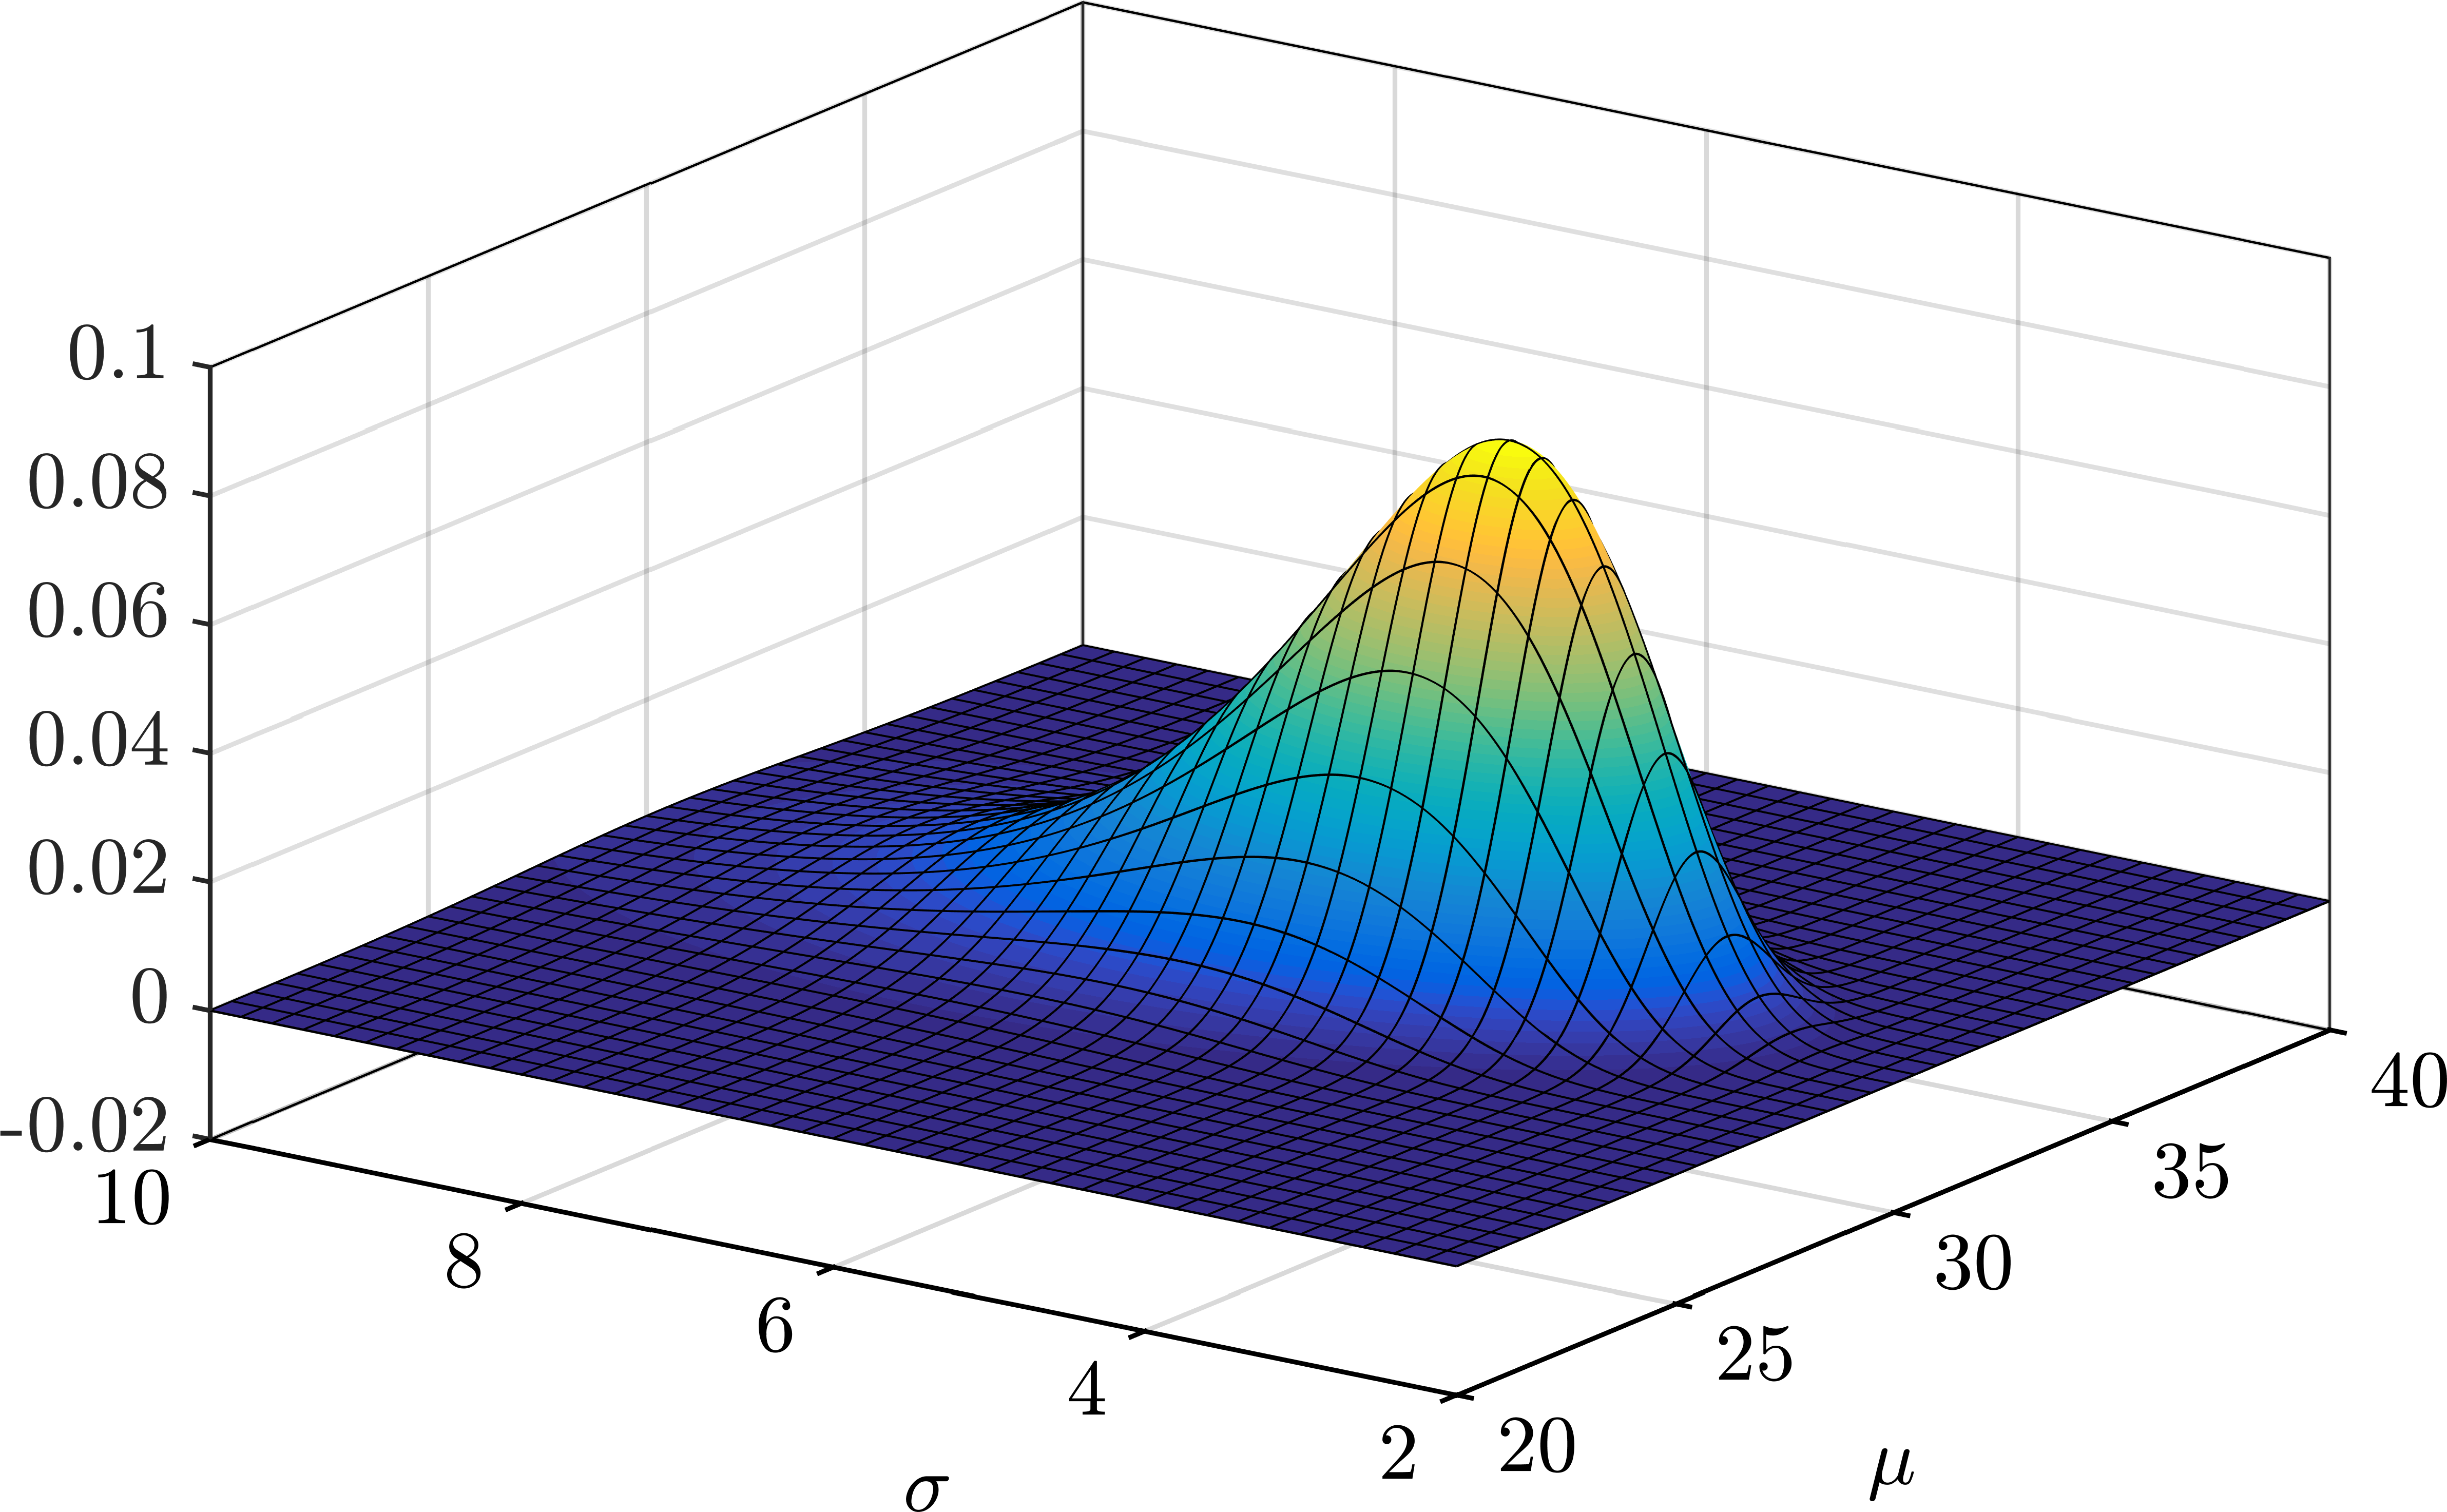
\includegraphics[width=\JCPfigWidth]{fig_JCP_Norm2D_Post3D_SLE}
    \caption{SLE with \(p = 50\).}
    \label{fig:JCP:Normal:Post3D:SLE}
  \end{subfigure}%
  \caption[2D normal fitting: Joint posterior]{2D normal fitting: Joint posterior.}
  \label{fig:JCP:Normal:Post2D}
\end{figure}
\par % POSTERIOR MARGINALS
Now the posterior marginals \(\pi(\mu \cond \bm{y})\) and \(\pi(\sigma \cond \bm{y})\) are computed from the joint posterior.
On the one hand, samples from the posterior marginals are obtained by restricting the analysis to the corresponding components of the joint MCMC sample.
On the other hand, functional approximations of the posterior marginals are extracted based on sub-expansions \(\hat{\mathcal{L}}_{\mu,p}(\mu)\)
and \(\hat{\mathcal{L}}_{\sigma,p}(\sigma)\) of a joint SLE \(\hat{\mathcal{L}}_p(\mu,\sigma)\) as in \cref{eq:JCP:SLE:Marginal1D,eq:JCP:SLE:SubExpansion1D}.
For the SLEs with \(p = 9\) and \(p = 50\) the results are visualized in \cref{fig:JCP:Normal:Post1D}.
Histogram-based MCMC sample representations and functional SLE approximations of the marginal densities are shown, too.
As it can be seen, the marginal posteriors as obtained by MCMC and the SLE with \(p = 50\) exactly match each other.
For \(p = 9\) the posteriors marginals display some wavelike fluctuations in their tails.
% FIGURES: POSTERIOR MARGINALS
\begin{figure}[htbp]
  \centering
  \begin{subfigure}[b]{\JCPsubWidth}
    \centering
    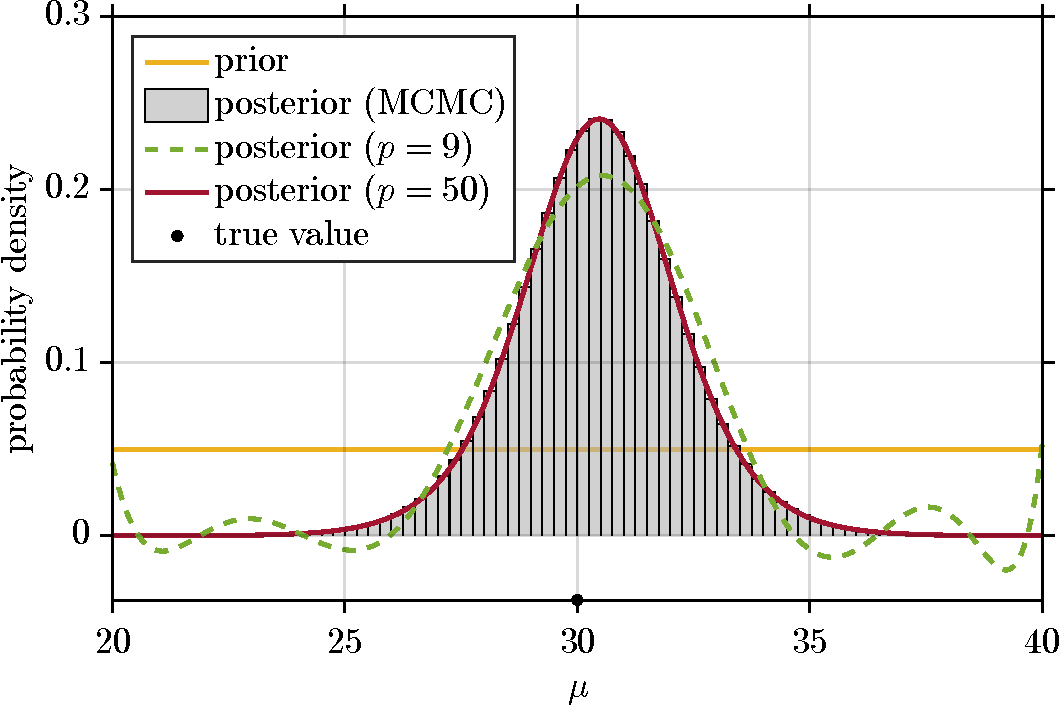
\includegraphics[height=\JCPfigHeight]{fig_JCP_Norm2D_Post1D_mu}
    \caption{Mean value \(\mu\).}
    \label{fig:JCP:Normal:Post1D:mu}
  \end{subfigure}\hfill%
  \begin{subfigure}[b]{\JCPsubWidth}
    \centering
    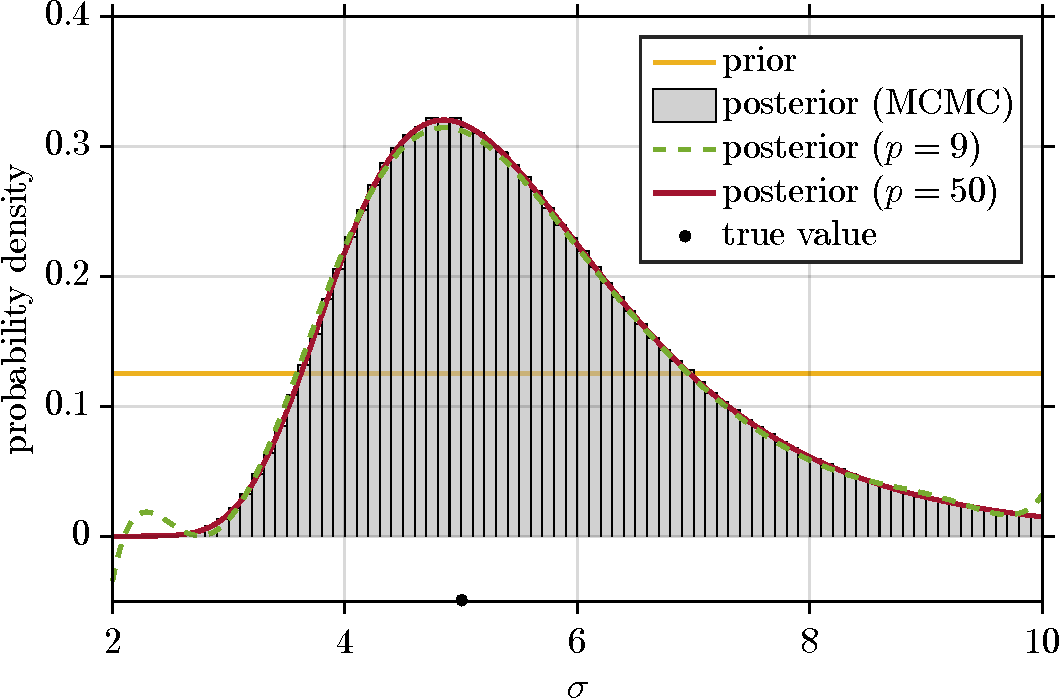
\includegraphics[height=\JCPfigHeight]{fig_JCP_Norm2D_Post1D_sigma}
    \caption{Standard deviation \(\sigma\).}
    \label{fig:JCP:Normal:Post1D:sigma}
  \end{subfigure}%
  \caption[2D normal fitting: Posterior marginals]{2D normal fitting: Posterior marginals.}
  \label{fig:JCP:Normal:Post1D}
\end{figure}

\subsubsection{Quantities of interest}
% STATISTICAL QUANTITIES OF INTEREST
Since the posterior density itself is of little inferential use, the model evidence and the first posterior moments are computed
for a selection of SLEs with varying size of the experimental design \(K\) and degree \(p\).
According to \cref{eq:JCP:SLE:ScaleFactor,eq:JCP:SLE:PosteriorMargMean,eq:JCP:SLE:PosteriorMargVariance,eq:JCP:SLE:PosteriorCovariance},
the SLE estimates of these quantities are obtained from the expansions coefficients.
In \cref{tab:JCP:Normal:StatisticalQuantities} a summary of the results is given.
Compliant with \cref{eq:JCP:SLE:ScaleFactor} the SLE estimates of the model evidence \(\scale\) are obtained as the coefficient of the constant expansion term.
According to \cref{eq:JCP:SLE:PosteriorMargMean,eq:JCP:SLE:PosteriorMargVariance}, the SLE estimates of the posterior mean \(\mathds{E}[\mu \cond \bm{y}]\)
and the standard deviation \(\mathrm{Std}[\mu \cond \bm{y}] = \mathrm{Var}[\mu \cond \bm{y}]^{1/2}\) of the location parameter \(\mu\) are computed.
Likewise, the corresponding estimates for the spread parameter \(\sigma\) follow through a simple postprocessing of the low-order expansion coefficients.
The SLE estimates of the linear coefficient of correlation
\(\rho[\mu,\sigma \cond \bm{y}] = \mathrm{Cov}[\mu,\sigma \cond \bm{y}] / \mathrm{Std}[\mu \cond \bm{y}] / \mathrm{Std}[\sigma \cond \bm{y}]\)
are computed based on \cref{eq:JCP:SLE:PosteriorCovariance}.
Additionally, the LOO error \(\epsilon_{\mathrm{LOO}}\) is listed to indicate the SLE prediction accuracy.
Note that all those estimates comply with the natural bounds and restrictions of the estimated quantities, e.g.\ the posterior means comply with the prior bounds.
\par % (MC)MC
For the sake of comparison, associated results are listed for the simulated MCMC sample, too.
These MCMC results are simply obtained as the corresponding sample approximations.
The reference estimate of the model evidence is obtained by crude MC simulation instead,
i.e.\ the arithmetic mean of the likelihood is computed for a number of \(10^8\) independent draws from the prior.
% DISCUSSION
It is interesting to note that the SLEs can reproduce the MCMC results for moderate experimental designs and degrees, say for \(K = 5 \times 10^3\) and \(p = 21\).
Even though a large number of input samples and a large polynomial degree is necessary to reproduce the shape of the joint posterior density,
significantly smaller experimental designs and polynomial orders suffice to reproduce the first posterior moments.
% TABLE: STATISTICAL QUANTITIES
\begin{table}[htbp]
  \caption[2D normal fitting: Statistical quantities]{2D normal fitting: Statistical quantities.}
  \label{tab:JCP:Normal:StatisticalQuantities}
  \centering
  \begin{tabular}{cccccccccc}
    \toprule
    & \(K\) & \(p\) & \(\epsilon_{\mathrm{LOO}}\)
    & \(\scale\) \([10^{-14}]\) & \(\mathds{E}[\mu \cond \bm{y}]\) & \(\mathds{E}[\sigma \cond \bm{y}]\)
    & \(\mathrm{Std}[\mu \cond \bm{y}]\) & \(\mathrm{Std}[\sigma \cond \bm{y}]\) & \(\rho[\mu,\sigma \cond \bm{y}]\) \\
    \midrule
    \multirow{6}{*}{\rotatebox[origin=c]{90}{SLE}}
    & \(5 \times 10^2\) & \(5\)  & \(4.24 \times 10^{-1}\) & \(1.19\) & \(30.34\) & \(5.57\) & \(2.03\) & \(1.39\) & \(\phantom{-}0.18\) \\
    & \(1 \times 10^3\) & \(9\)  & \(1.19 \times 10^{-1}\) & \(1.20\) & \(30.39\) & \(5.54\) & \(2.01\) & \(1.41\) & \(\phantom{-}0.08\) \\
    & \(5 \times 10^3\) & \(21\) & \(9.64 \times 10^{-4}\) & \(1.18\) & \(30.48\) & \(5.56\) & \(1.79\) & \(1.38\) & \(-0.01\) \\
    & \(1 \times 10^4\) & \(32\) & \(5.86 \times 10^{-6}\) & \(1.18\) & \(30.47\) & \(5.56\) & \(1.81\) & \(1.38\) & \(\phantom{-}0.00\) \\
    & \(5 \times 10^4\) & \(45\) & \(1.30 \times 10^{-9}\) & \(1.18\) & \(30.47\) & \(5.56\) & \(1.81\) & \(1.38\) & \(-0.00\) \\
    & \(1 \times 10^5\) & \(50\) & \(\phantom{^{1}}6.05 \times 10^{-11}\) & \(1.18\) & \(30.47\) & \(5.56\) & \(1.81\) & \(1.38\) & \(-0.00\) \\
    \midrule
    \multicolumn{4}{c}{(MC)MC}                             & \(1.18\) & \(30.47\) & \(5.56\) & \(1.81\) & \(1.38\) & \(-0.00\) \\
    \bottomrule
  \end{tabular}
\end{table}

\subsection{2D inverse heat conduction}
% INVERSE HEAT CONDUCTION
Finally, an inverse heat conduction problem (IHCP) is considered.
The heat equation is a partial differential equation (PDE) that describes the distribution and evolution of heat in a system where conduction is the dominant mode of heat transfer.
We consider a stationary heat equation of the form
\begin{equation} \label{eq:JCP:Heat:Stationary}
  \nabla \cdot (\kappa \nabla \perfect{T}) = 0.
\end{equation}
The temperature is denoted as \(\perfect{T}\) and the thermal conductivity is denoted as \(\kappa\).
Commonly one is interested in the solution of the boundary value problem that is posed when \cref{eq:JCP:Heat:Stationary} is satisfied over a physical domain subject to appropriate boundary conditions.
We consider the steady state situation in two spatial dimensions.
The Euclidean coordinate vector is denoted as \(\bm{r} = (r_1,r_2)^\top\) in the following.
\par % PROBLEM SETUP
It is dealt with the identification of thermal conductivities of inclusions in a composite material with close-to-surface measurements of the temperature.
The setup of the simplified thermal problem is visualized in \cref{fig:JCP:Heat:HeatConduction2D}.
The thermal conductivity of the background matrix is denoted as \(\kappa_0\), while the conductivities of the material inclusions are termed as \(\kappa_1\) and \(\kappa_2\), respectively.
It is assumed that the material properties are not subject to a further spatial variability.
% BOUNDARY CONDITIONS
At the ``top'' of the domain a Dirichlet boundary condition \(\perfect{T}_1\) is imposed,
while at the ``bottom'' the Neumann boundary condition \(q_2 = - \kappa_0 \, \partial \perfect{T} / \partial r_2\) is imposed.
Zero heat flux conditions \(\partial \perfect{T} / \partial r_1 = 0\) are imposed at the ``left'' and ``right'' hand side.
\par % INVERSE PROBLEM
We consider the IHCP that is posed when the thermal conductivities \(\bm{\kappa} = (\kappa_1,\kappa_2)^\top\) are unknown and their inference is intended.
With this in mind, a number of \(\dimData\) measurements \(\bm{T} = (T(\bm{r}_1),\ldots,T(\bm{r}_\dimData))^\top\)
of the temperature field at the measurement locations \((\bm{r}_1,\ldots,\bm{r}_\dimData)\) is available.
The forward model \(\mathcal{M} \colon \bm{\kappa} \mapsto \perfect{\bm{T}}\) establishes the connection between the data and the unknowns.
It formalizes the operation of solving \cref{eq:JCP:Heat:Stationary} for \(\perfect{\bm{T}}\) as a function of \(\bm{\kappa}\).
Measured temperatures \(\bm{T} = \perfect{\bm{T}} + \bm{\varepsilon}\) consist of the corresponding model response \(\perfect{\bm{T}} = \mathcal{M}(\bm{\kappa})\) and a residual term \(\bm{\varepsilon}\).
The latter accounts for measurement uncertainty and forward model inadequacy.
We consider residuals that are distributed according to a Gaussian \(\mathcal{N}(\bm{\varepsilon} \cond \bm{0},\bm{\Sigma})\) with covariance matrix \(\bm{\Sigma}\).
In compliance with \cref{eq:JCP:Bayesian:Inverse:Likelihood} the likelihood function is given as \(\mathcal{L}(\bm{\kappa}) = \mathcal{N}(\bm{T} \cond \mathcal{M}(\bm{\kappa}),\bm{\Sigma})\).
Provided that a prior distribution \(\pi(\bm{\kappa})\) can be elicited, the posterior is given as \(\pi(\bm{\kappa} \cond \bm{T}) = \scale^{-1} \mathcal{L}(\bm{\kappa}) \pi(\bm{\kappa})\).
\par % EXPERIMENTAL SETUP
The thermal conductivity of the background matrix is set to \(\kappa_0 = \unit[15]{W/m/K}\),
while the thermal conductivities of the inclusions are specified as \(\kappa_1 = \unit[32]{W/m/K}\) and \(\kappa_1 = \unit[28]{W/m/K}\).
The material properties of the inclusions are treated as unknowns subsequently.
Moreover, the boundary conditions \(\perfect{T}_1 = \unit[200]{K}\) and \(q_2 = \unit[2000]{W/m^2}\) are imposed.
A finite element (FE) model is used to solve a weak form of the governing PDE.
The FE solution for the experimental setup described above is shown in \cref{fig:JCP:Heat:SteadyState2D}.
We consider a uniform prior distribution \(\pi(\bm{\kappa}) = \pi(\kappa_1) \pi(\kappa_2)\) with independent marginals
\(\pi(\kappa_1) = \mathcal{U}(\kappa_1 \cond \underline{\kappa}_1,\overline{\kappa}_1)\) and \(\pi(\kappa_2) = \mathcal{U}(\kappa_2 \cond \underline{\kappa}_2,\overline{\kappa}_2)\).
The prior bounds are chosen as \(\underline{\kappa}_1 = \underline{\kappa}_2 = \unit[20]{W/m/K}\) and \(\overline{\kappa}_1 = \overline{\kappa}_2 = \unit[40]{W/m/K}\), respectively.
A number of \(\dimData = 12\) close-to-surface observations is analyzed.
Their measurement locations are indicated by the black dots in \cref{fig:JCP:Heat:HeatConduction2D}.
Independent Gaussian measurement noise with \(\bm{\Sigma} = \sigma_T^2 \bm{1}\) and \(\sigma_T = \unit[0.25]{K}\) is considered.
Based on this setup, synthetic data are simulated for conducting the computer experiment.
This means that the forward model responses \(\perfect{\bm{T}}\) for the true parameter setup are computed and pseudo-random noise is added in order to obtain \(\bm{T}\).
% FIGURES: PDE & FEM
\begin{figure}[htbp]
  \begin{minipage}[b]{\JCPsubWidth}
    \centering
    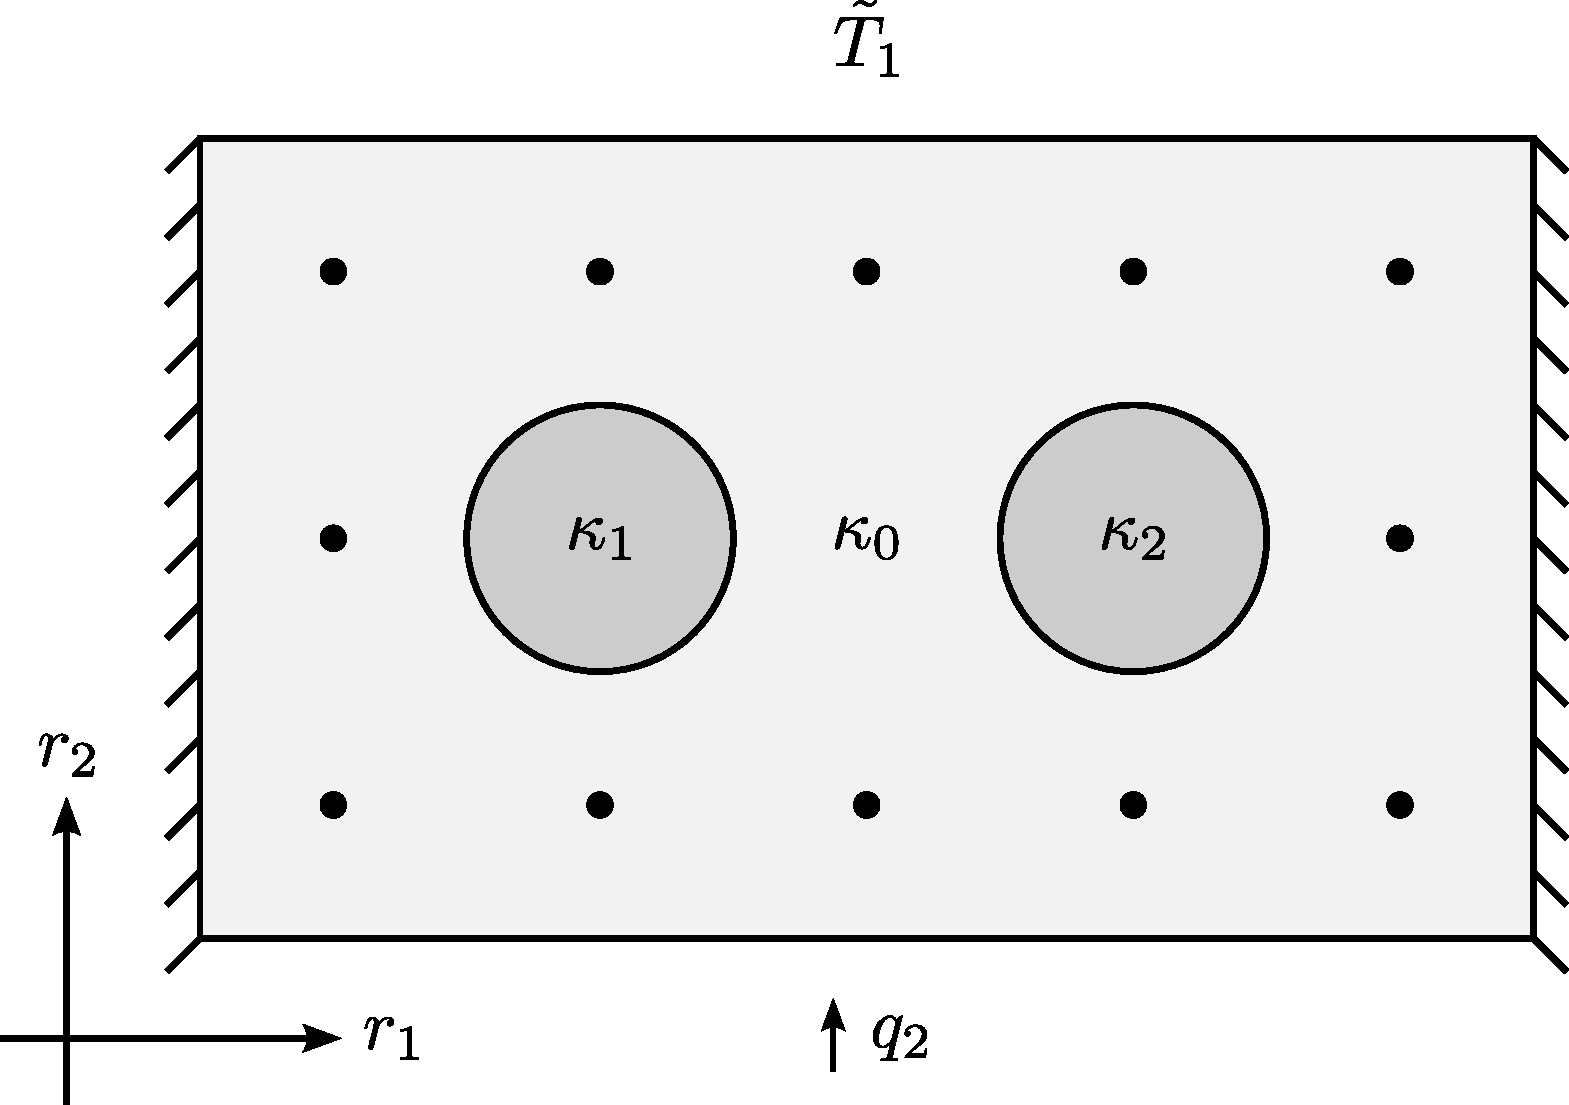
\includegraphics[height=\JCPfigHeight]{fig_JCP_Heat2D_HeatConduction}
    \caption[2D IHCP: Heat conduction setup]{2D IHCP: Heat conduction setup.}
    \label{fig:JCP:Heat:HeatConduction2D}
  \end{minipage}%
  \hfill%
  \begin{minipage}[b]{\JCPsubWidth}
    \centering
    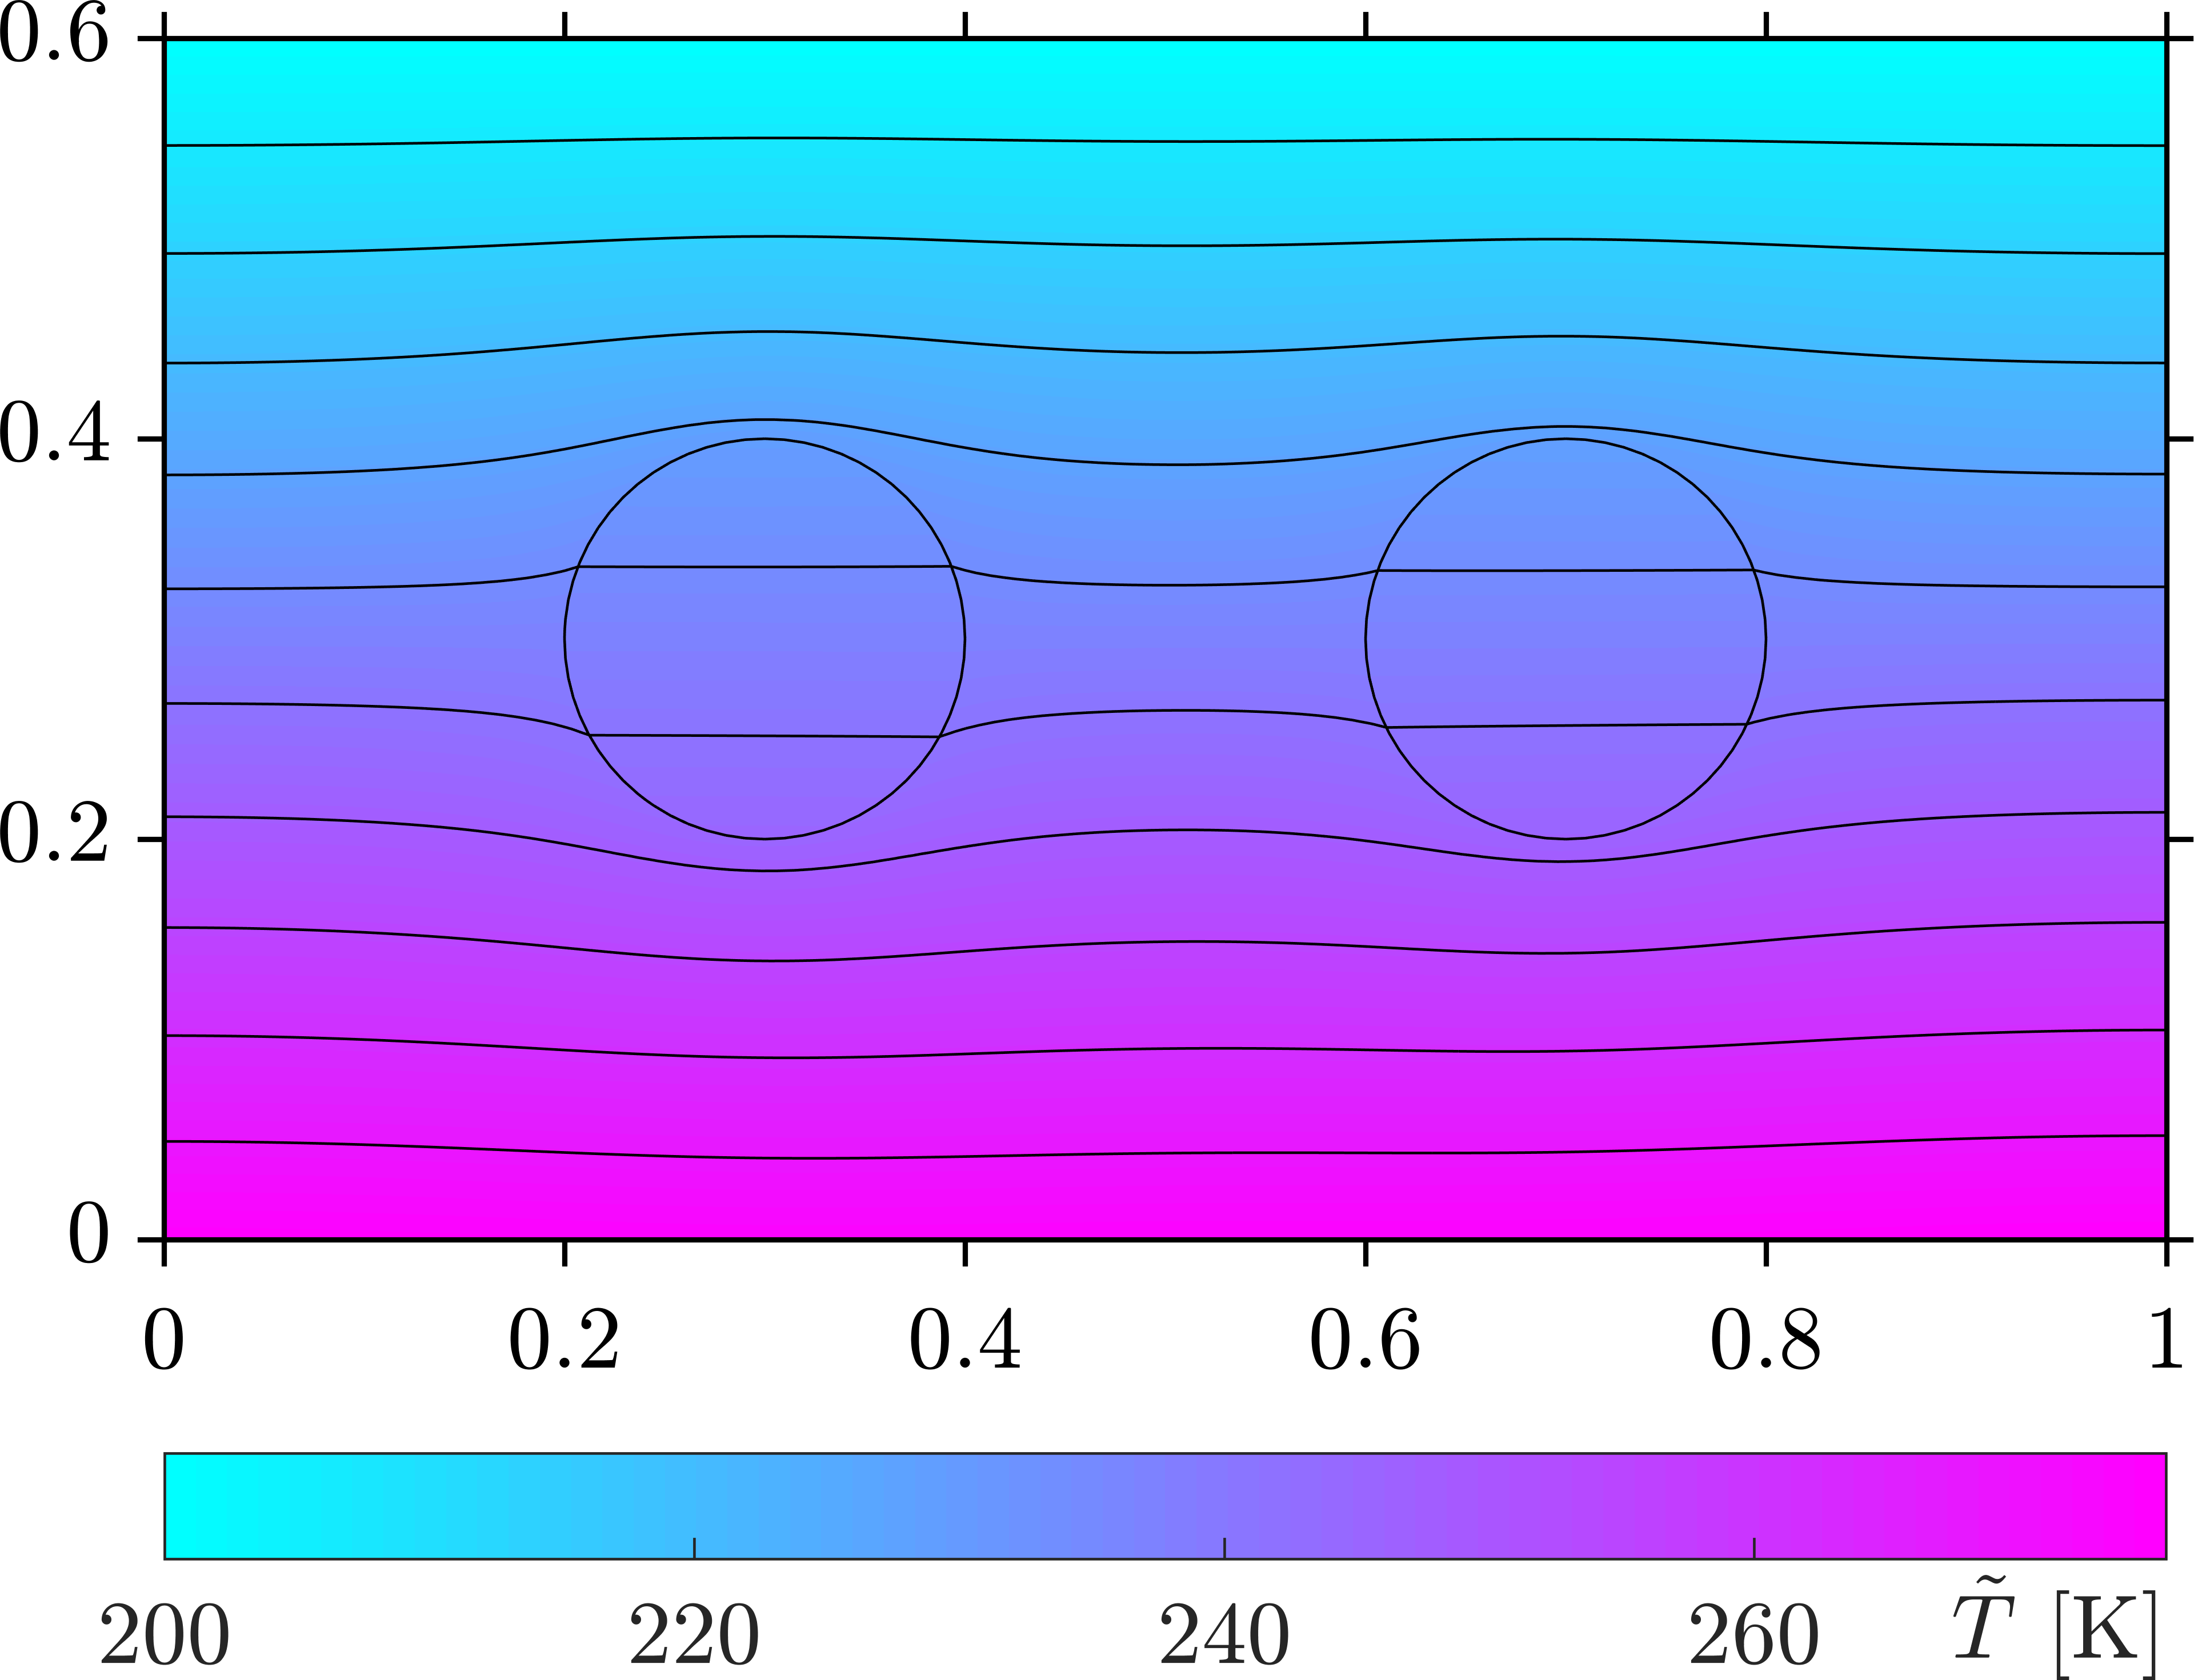
\includegraphics[height=\JCPfigHeight]{fig_JCP_Heat2D_SteadyState}
    \caption[2D IHCP: Steady state solution]{2D IHCP: Steady state solution.}
    \label{fig:JCP:Heat:SteadyState2D}
  \end{minipage}%
\end{figure}

\subsubsection{Posterior density}
% COMPARISON TO 2D GAUSSIAN
The analyses proceed analogously to the preceding section.
By comparing the present IHCP and the non-conjugate Gaussian example, that have a two-dimensional parameter space and uniform priors in common,
one can gain interesting insight into spectral Bayesian inference.
% SLE CONVERGENCE
First, the convergence behavior of the SLE is investigated.
Spectral expansions \(\hat{\mathcal{L}}_p\) of the likelihood \(\mathcal{L}\) are therefore computed
for an experimental design of size \(K = 1 \times 10^5\) and candidate bases with polynomials up to degree \(p = 50\).
All practical issues are handled analogously to the procedure in the non-conjugate Gaussian example.
In \cref{fig:JCP:Heat:ConvSLE} the normalized versions of the empirical error \(\epsilon_{\mathrm{Emp}}\) and the LOO error \(\epsilon_{\mathrm{LOO}}\) are shown as a function of \(p\).
Comparing these results to \cref{fig:JCP:Normal:ConvSLE} reveals that the convergence rate of the SLE \(\hat{\mathcal{L}}_p\) is considerably slower than the corresponding one for the Gaussian example.
For the SLE with \(p = 50\) the error estimates amount to \(\epsilon_{\mathrm{Emp}} = 6.26 \times 10^{-4}\) and \(\epsilon_{\mathrm{LOO}} = 7.56 \times 10^{-4}\).
These errors are around seven orders of magnitude higher than the errors observed for the Gaussian example.
% DIFFERENT CONVERGENCE RATE
The difference in the SLE convergence rate presumably originates from a difference in the underlying likelihood functions and posterior densities.
This is now investigated in more detail.
% FIGURE: SLE CONVERGENCE
\begin{figure}[htbp]
  \centering
  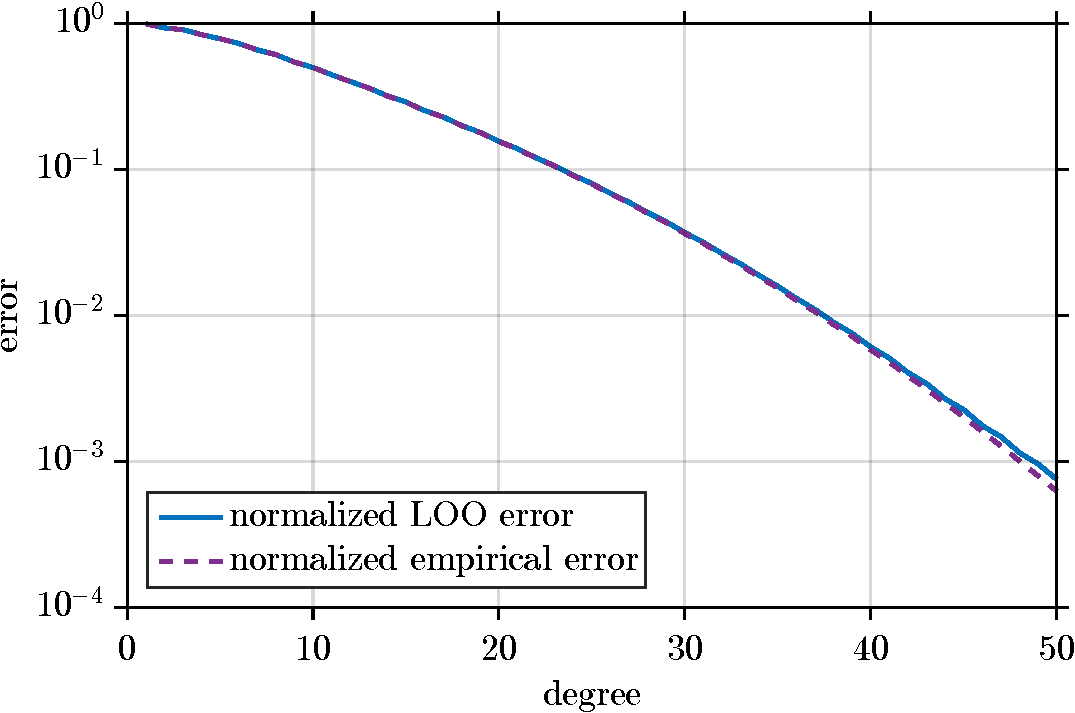
\includegraphics[height=\JCPfigHeight]{fig_JCP_Heat2D_ConvSLE}
  \caption[2D IHCP: Convergence of the SLE]{2D IHCP: Convergence of the SLE.}
  \label{fig:JCP:Heat:ConvSLE}
\end{figure}
\par % POSTERIOR DENSITY
A RWM approximation with \(10^7\) samples and the SLE-based emulation with \(p = 50\) of the posterior density
\(\pi(\kappa_1,\kappa_2 \cond \bm{T}) \approx \coeffL_{\bm{0}}^{-1} \hat{\mathcal{L}}_p(\kappa_1,\kappa_2) \pi(\kappa_1,\kappa_2)\) are depicted in \cref{fig:JCP:Heat:Post2D}.
% FORWARD MODEL SURROGATE
In order to reduce the numerical cost of MCMC sampling, the FE model \(\mathcal{M}\) is replaced by a PCE surrogate \(\hat{\mathcal{M}}_p\).
For \(i = 1,\ldots,\dimData\), separate PCEs \(\hat{\mathcal{M}}_{i,p}\) of the temperature \(\perfect{T}_i = \mathcal{M}_{i,p}(\kappa_1,\kappa_2)\)
at the location \(\bm{r}_i\) are fitted as a function of the unknown conductivities.
After an appropriate transformation to standardized variables, tensorized Legendre polynomials up to degree \(p = 10\) act as the trial basis.
Based on an experimental design of the size \(K = 10^3\), the LOO errors of the regressions amount to about \(\epsilon_{\mathrm{LOO}} \approx 10^{-10}\).
Accordingly, the PCE is considered an adequate replacement of the full FE model.
% TWO-STAGE REGRESSION
Note that it would be also possible to use \(\hat{\mathcal{M}}_p\) as a forward model surrogate during the likelihood training runs.
\par % POSTERIOR DENSITY
The posteriors in \cref{fig:JCP:Heat:Post2D} can be compared to the posteriors of the Gaussian example in \cref{fig:JCP:Normal:Post2D} of the previous section.
Relative to the respective prior, the posterior of the thermal problem \(\pi(\kappa_1,\kappa_2 \cond \bm{T})\)
contains more information than the posterior of the normal problem \(\pi(\mu,\sigma \cond \bm{y})\),
i.e.\ the likelihood \(\mathcal{L}(\kappa_1,\kappa_2)\) has a slightly more peaked and localized structure than \(\mathcal{L}(\mu,\sigma)\).
In order to capture these different behaviors nearby and far from the posterior mode,
the SLEs \(\hat{\mathcal{L}}_p(\kappa_1,\kappa_2)\) and \(\hat{\mathcal{L}}_p(\mu,\sigma)\) require a different number of expansions terms.
The more localized the posterior modes are with respect to the prior, the more terms are required in order to achieve the cancellation in the tails.
Moreover, as opposed to \(\pi(\mu,\sigma \cond \bm{y})\) the posterior \(\pi(\kappa_1,\kappa_2 \cond \bm{T})\) exhibits a pronounced correlation structure.
In turn, this requires non-vanishing interaction terms.
As a consequence, the SLE \(\hat{\mathcal{L}}_p(\kappa_1,\kappa_2)\) of the IHCP example is less accurate than the SLE \(\hat{\mathcal{L}}_p(\mu,\sigma)\) of the Gaussian example.
This is also reflected in the fact that the posterior surrogate fluctuates and takes on negative values
around the points \([\underline{\kappa}_1,\underline{\kappa}_2]\) and \([\overline{\kappa}_1,\overline{\kappa}_2]\).
In order to see this more clearly, the SLE posterior surrogate from \cref{fig:JCP:Heat:Post2D:SLE} is plotted again from a different angle in \cref{fig:JCP:Heat:Post3D:SLE}.
A small wavelike posterior structure spans the parameter space between these corners.
These artifacts stem from an imperfect polynomial cancellation of the finite series approximation.
This stands in contrast to the posterior of the Gaussian example in \cref{fig:JCP:Normal:Post3D:SLE} where these phenomena were not observed.
% FIGURES: 2D POSTERIORS
\begin{figure}[htbp]
  \centering
  \begin{subfigure}[b]{\JCPsubWidth}
    \centering
    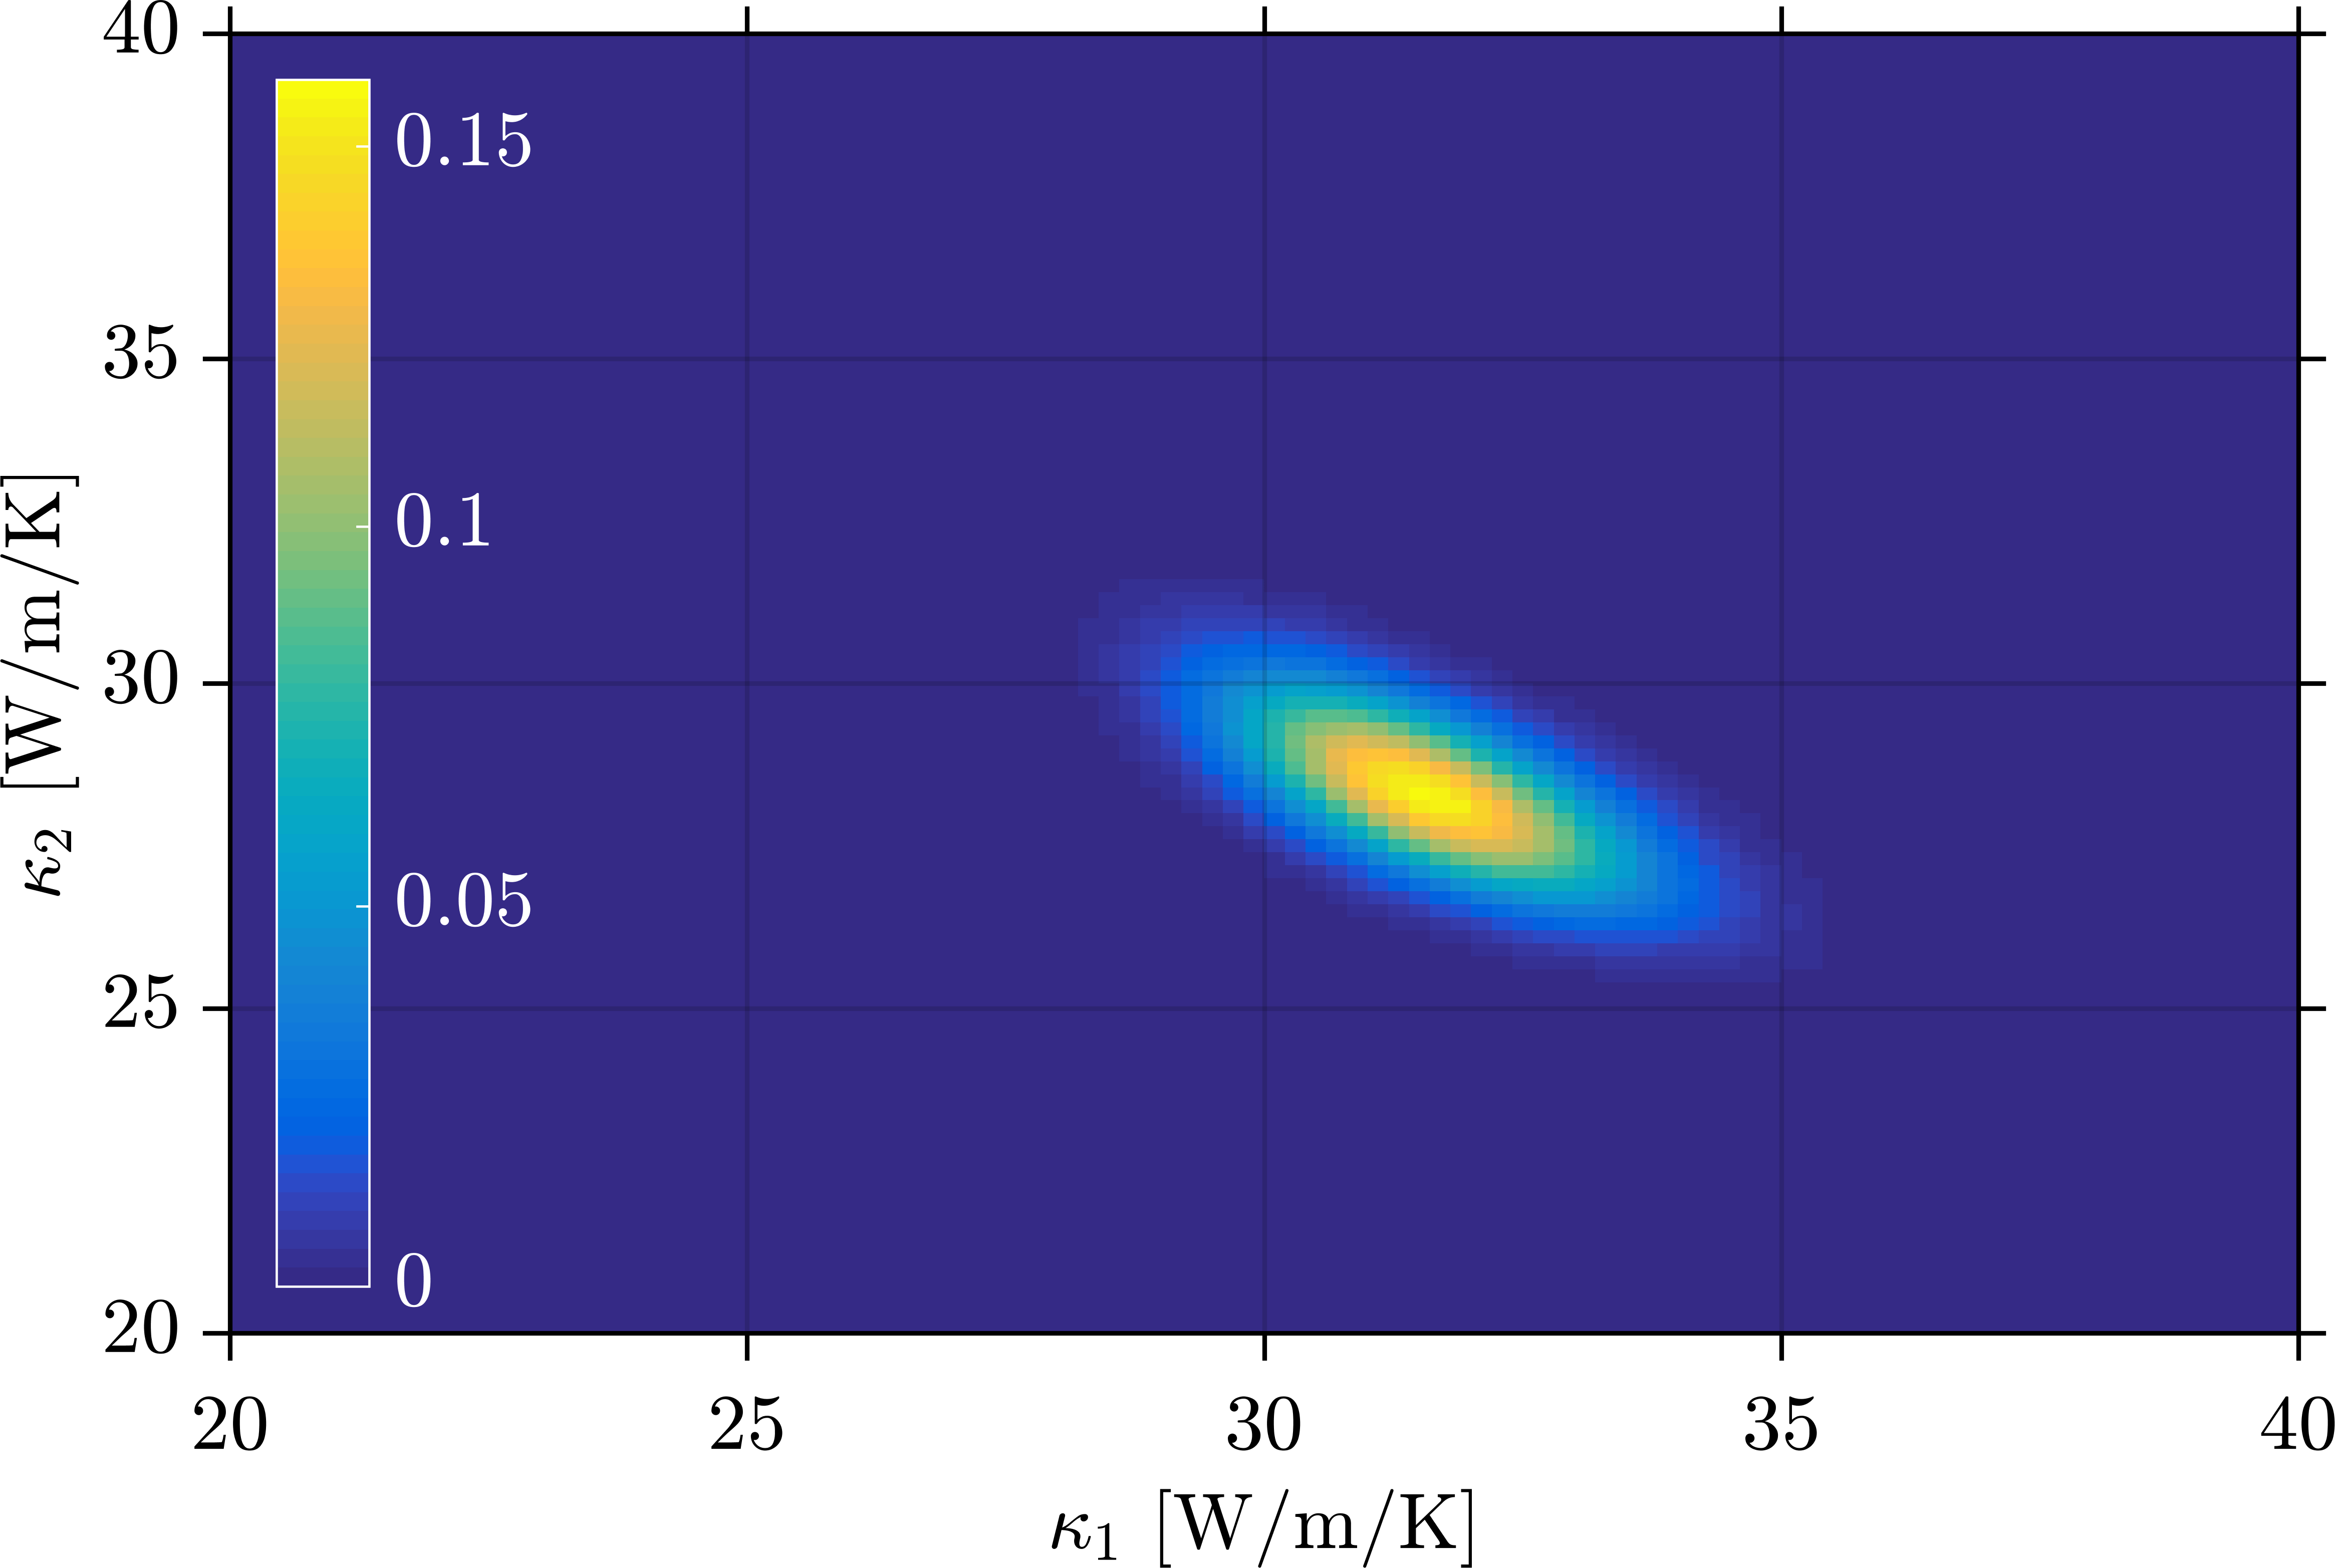
\includegraphics[height=\JCPfigHeight]{fig_JCP_Heat2D_Post2D_MCMC}
    \caption{MCMC reference sample.}
    \label{fig:JCP:Heat:Post2D:MCMC}
  \end{subfigure}\hfill%
  \begin{subfigure}[b]{\JCPsubWidth}
    \centering
    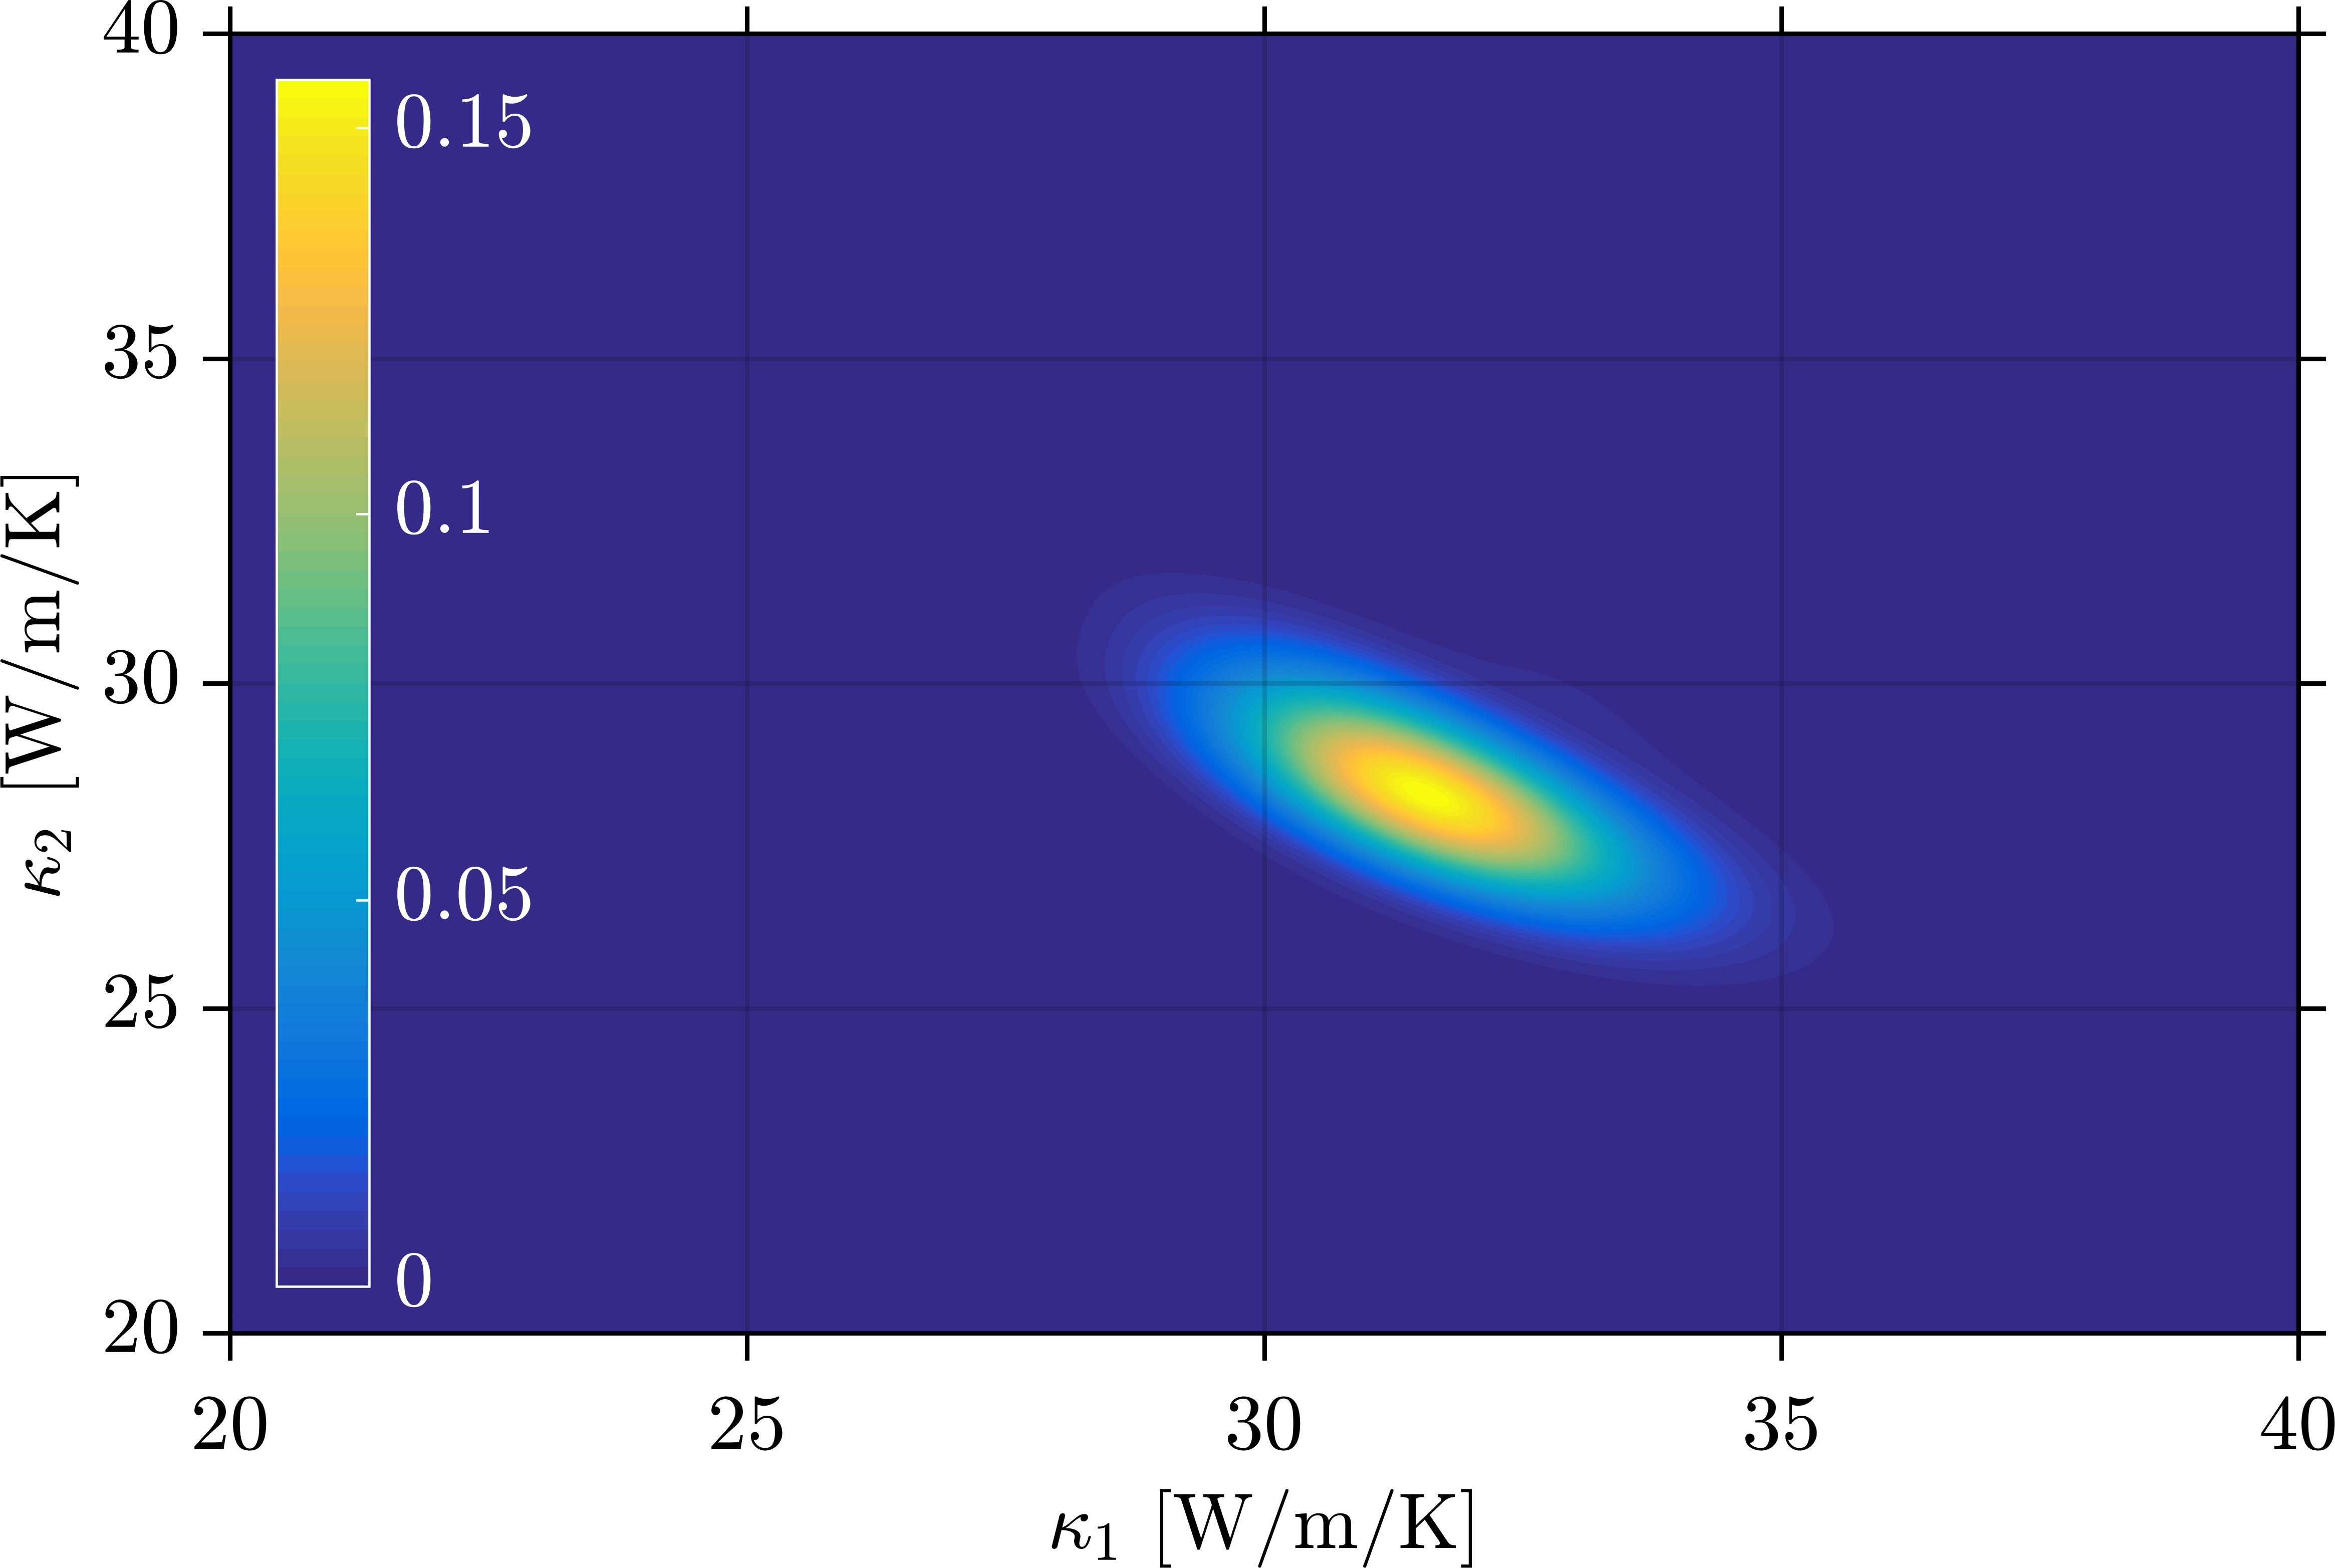
\includegraphics[height=\JCPfigHeight]{fig_JCP_Heat2D_Post2D_SLE}
    \caption{SLE with \(p = 50\).}
    \label{fig:JCP:Heat:Post2D:SLE}
  \end{subfigure}\\[1ex]%
  \begin{subfigure}[b]{\JCPsubWidth}
    \centering
    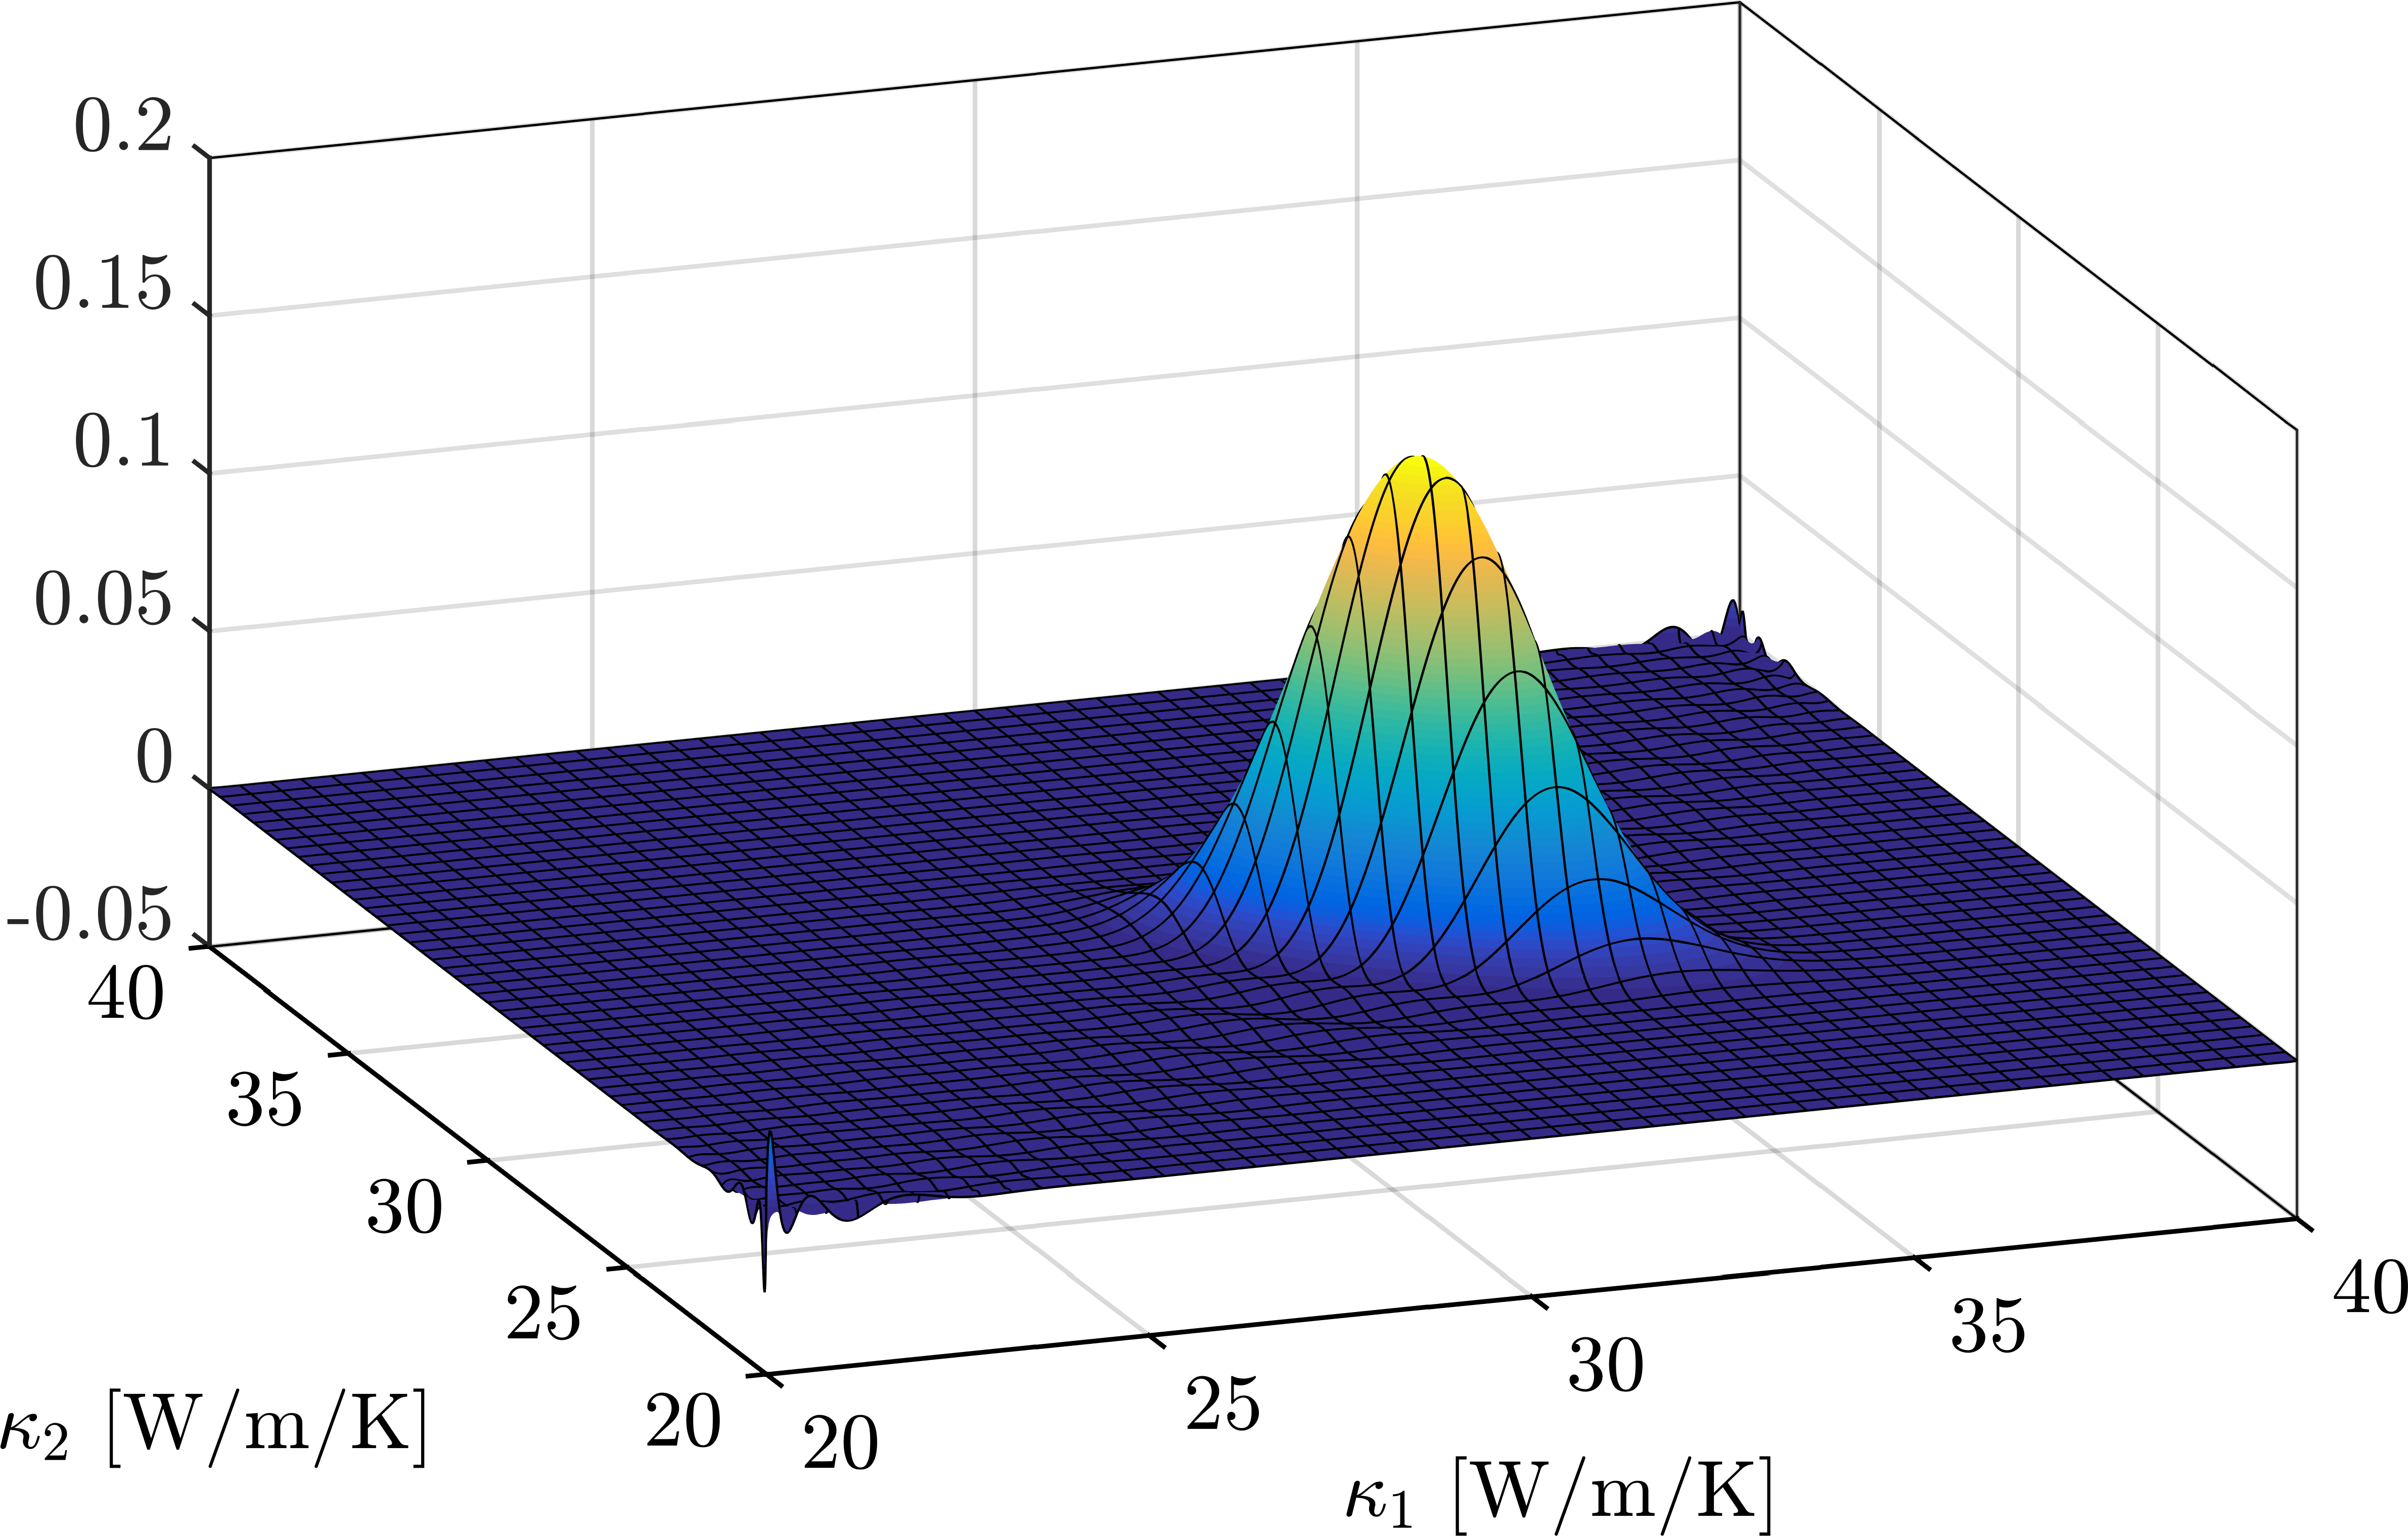
\includegraphics[width=\JCPfigWidth]{fig_JCP_Heat2D_Post3D_SLE}
    \caption{SLE with \(p = 50\).}
    \label{fig:JCP:Heat:Post3D:SLE}
  \end{subfigure}%
  \caption[2D IHCP: Joint posterior]{2D IHCP: Joint posterior.}
  \label{fig:JCP:Heat:Post2D}
\end{figure}
\par % POSTERIOR MARGINALS
Via \cref{eq:JCP:SLE:Marginal1D} the posterior marginals \(\pi(\kappa_1 \cond \bm{T})\) and \(\pi(\kappa_2 \cond \bm{T})\) can be extracted from the joint SLEs.
The resulting densities are shown in \cref{fig:JCP:Heat:Post1D} together with a histogram-based MCMC sample representation.
As it can be seen, for \(p = 50\) the marginals are captured fairly well,
while the moderate-order surrogate for \(p = 21\) still exhibits discrepancies at the bounds of the parameter space.
The approximation of the posterior marginals by sub-SLEs seems to be more accurate, at least in the sense of the maximum deviation,
than the approximation of the joint posterior \(\pi(\kappa_1,\kappa_2 \cond \bm{T})\) by the full SLE in \cref{fig:JCP:Heat:Post3D:SLE}.
This phenomenon can be explained through the absence of all non-constant polynomial terms in the variables that are marginalized out.
% FIGURES: POSTERIOR MARGINALS
\begin{figure}[htbp]
  \centering
  \begin{subfigure}[b]{\JCPsubWidth}
    \centering
    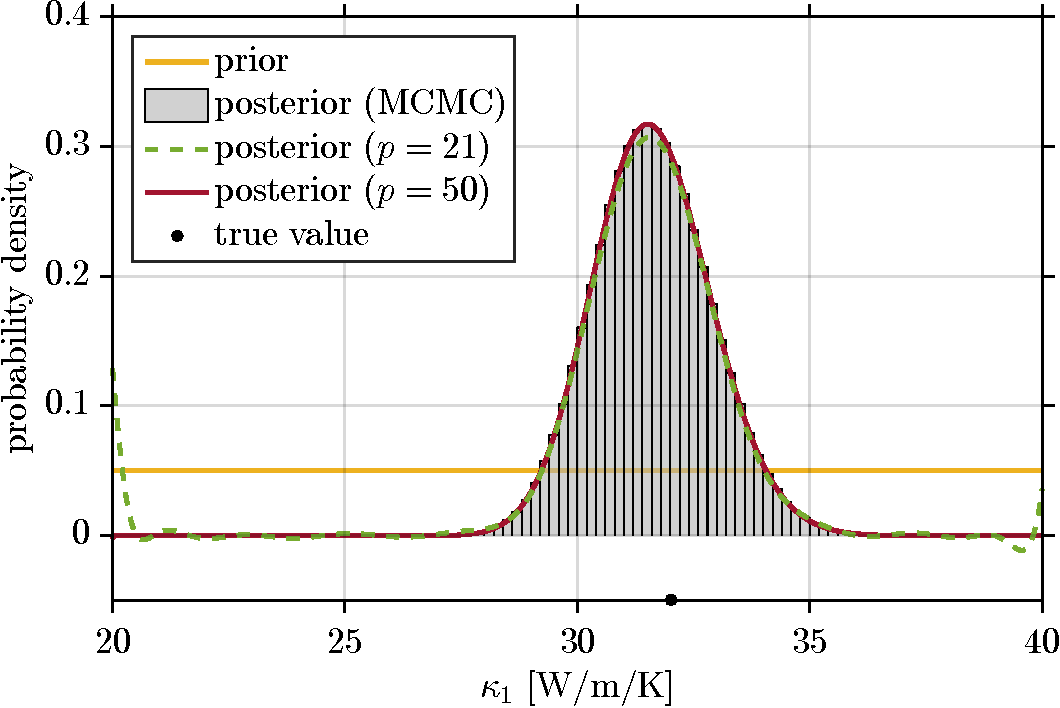
\includegraphics[height=\JCPfigHeight]{fig_JCP_Heat2D_Post1D_k1}
    \caption{Thermal conductivity \(\kappa_1\).}
    \label{fig:JCP:Heat:Post1D:k1}
  \end{subfigure}\hfill%
  \begin{subfigure}[b]{\JCPsubWidth}
    \centering
    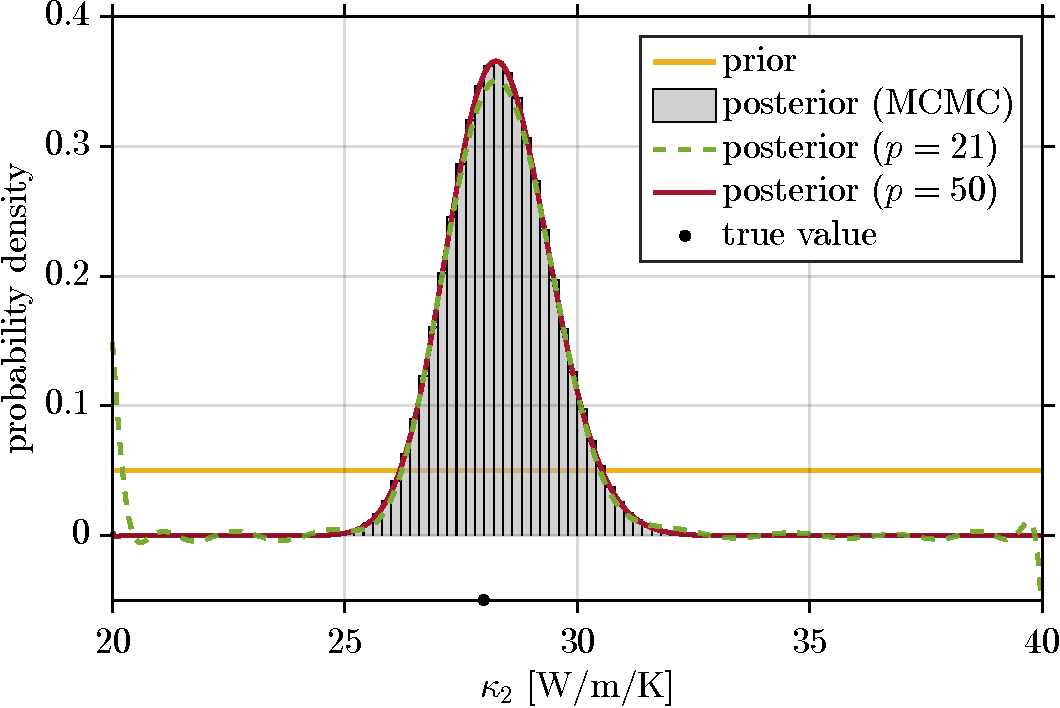
\includegraphics[height=\JCPfigHeight]{fig_JCP_Heat2D_Post1D_k2}
    \caption{Thermal conductivity \(\kappa_2\).}
    \label{fig:JCP:Heat:Post1D:k2}
  \end{subfigure}%
  \caption[2D IHCP: Posterior marginals]{2D IHCP: Posterior marginals.}
  \label{fig:JCP:Heat:Post1D}
\end{figure}

\subsubsection{Quantities of interest}
% STATISTICAL QUANTITIES OF INTEREST
Now we investigate how well one can extract the statistically interesting quantities.
Results from SLEs with varying \(K\) and \(p\) are compared with the results from MCMC sampling.
A summary of the findings is provided in \cref{tab:JCP:Heat:StatisticalQuantities}.
The LOO error \(\epsilon_{\mathrm{LOO}}\) of various SLEs is shown together with some basic posterior characteristics obtained by a postprocessing of the SLE coefficients.
For \(j = 1,2\) the posterior mean \(\mathds{E}[\kappa_j \cond \bm{T}]\) and the standard deviation \(\mathrm{Std}[\kappa_j \cond \bm{T}] = \mathrm{Var}[\kappa_j \cond \bm{T}]^{1/2}\)
of the posterior distribution are given in physical units of \(\unit[]{W/m/K}\).
In addition, the model evidence \(\scale\) and the linear coefficient of correlation
\(\rho[\kappa_1,\kappa_2 \cond \bm{T}] = \mathrm{Cov}[\kappa_1,\kappa_2 \cond \bm{T}] / \mathrm{Std}[\kappa_1 \cond \bm{T}] / \mathrm{Std}[\kappa_2 \cond \bm{T}]\) are specified.
% DISCUSSION
In comparison to \cref{tab:JCP:Normal:StatisticalQuantities}, where the results for the non-conjugate normal example are listed, the SLE results for the IHCP match their MCMC counterparts less accurately.
Nevertheless, it can be observed that the lowest-degree quantities of inferential interest can be extracted with a comparably small experimental design and relatively low number of regressors,
say with \(K = 1 \times 10^4\) and \(p = 29\).
Note that all the estimates attain admissible values.
% TABLE: STATISTICAL QUANTITIES
\begin{table}[htbp]
  \caption[2D IHCP: Statistical quantities]{2D IHCP: Statistical quantities.}
  \label{tab:JCP:Heat:StatisticalQuantities}
  \centering
  \begin{tabular}{cccccccccc}
    \toprule
    & \(K\) & \(p\) & \(\epsilon_{\mathrm{LOO}}\)
    & \(\scale\) \([10^{-1}]\) & \(\mathds{E}[\kappa_1 \cond \bm{T}]\) & \(\mathds{E}[\kappa_2 \cond \bm{T}]\)
    & \(\mathrm{Std}[\kappa_1 \cond \bm{T}]\) & \(\mathrm{Std}[\kappa_2 \cond \bm{T}]\) & \(\rho[\kappa_1,\kappa_2 \cond \bm{T}]\) \\
    \midrule
    \multirow{6}{*}{\rotatebox[origin=c]{90}{SLE}}
    & \(5 \times 10^2\) & \(5\)  & \(8.24 \times 10^{-1}\) & \(8.45\) & \(31.33\) & \(28.36\) & \(1.74\) & \(1.33\) & \(\phantom{-}0.28\) \\
    & \(1 \times 10^3\) & \(9\)  & \(6.08 \times 10^{-1}\) & \(7.81\) & \(31.40\) & \(28.22\) & \(2.02\) & \(1.53\) & \(\phantom{-}0.15\) \\
    & \(5 \times 10^3\) & \(21\) & \(1.50 \times 10^{-1}\) & \(7.47\) & \(31.32\) & \(28.13\) & \(2.16\) & \(1.61\) & \(\phantom{-}0.34\) \\
    & \(1 \times 10^4\) & \(29\) & \(5.79 \times 10^{-2}\) & \(7.21\) & \(31.56\) & \(28.30\) & \(1.61\) & \(1.39\) & \(-0.05\) \\
    & \(5 \times 10^4\) & \(35\) & \(1.63 \times 10^{-2}\) & \(7.18\) & \(31.62\) & \(28.34\) & \(1.24\) & \(1.08\) & \(-0.75\) \\
    & \(1 \times 10^5\) & \(50\) & \(7.56 \times 10^{-4}\) & \(7.18\) & \(31.62\) & \(28.33\) & \(1.26\) & \(1.10\) & \(-0.68\) \\
    \midrule
    \multicolumn{4}{c}{(MC)MC}                             & \(7.17\) & \(31.62\) & \(28.33\) & \(1.26\) & \(1.09\) & \(-0.68\) \\
    \bottomrule
  \end{tabular}
\end{table}

\subsection{6D inverse heat conduction}
% PROOF OF CONCEPT
In the previous sections it was demonstrated that likelihood functions can be indeed spectrally expanded and that the posterior density with its moments can be computed accordingly.
For low-dimensional problems the SLE convergence behavior up to a high degree was studied by monitoring the LOO error.
It was shown that the expansion error can be arbitrarily reduced by increasing the order of the expansion and adding samples to the experimental design.
% HIGHER DIMENSIONAL
While this is reassuring to know, it does not help in solving higher-dimensional problems
for which the computation of high-order expansions is exacerbated by the curse of dimensionality.
Hence, now we want to investigate the applicability of SLEs and aSLEs in an inverse problem of moderate dimension.
\par % PROBLEM SETUP
An IHCP in two spatial dimensions with six unknown conductivities is considered in this section.
The setup of the problem is shown in \cref{fig:JCP:Thermal:HeatConduction}.
The \(\dimParam = 6\) unknown conductivities \(\bm{\kappa} = (\kappa_1,\ldots,\kappa_6)^\top\) are inferred
with \(\dimData = 20\) noisy measurements \(\bm{T} = (T_{1},\ldots,T_{20})^\top\) of the temperature field \(\perfect{T}\).
% EXPERIMENTAL SETUP
We set \(\kappa_0 = \unit[30]{W/m/K}\) and \(\bm{\kappa} = \unit[(20,24,\ldots,40)^\top]{W/m/K}\).
The prior is set to a multivariate lognormal distribution \(\pi(\bm{\kappa}) = \prod_{i=1}^6 \pi(\kappa_i)\) with independent marginals
\(\pi(\kappa_i) = \mathcal{LN}( \kappa_i \cond \mu_0,\sigma_0^2)\) with \(\mu_0 = \unit[30]{W/m/K}\) and \(\sigma_0 = \unit[6]{W/m/K}\).
These parameters describe the mean \(\mu_0 = \mathds{E}[\kappa_i]\) and standard deviation \(\sigma_0 = \mathrm{Std}[\kappa_i]\) of the lognormal prior.
They are related to the parameters of the associated normal distribution \(\mathcal{N}( \log(\kappa_i) \cond \lambda_0,\varsigma_0^2)\)
via \(\mu_0 = \exp(\lambda_0 + \varsigma_0^2 / 2)\) and \(\sigma_0^2 = (\exp(\varsigma_0^2) - 1) \exp(2 \lambda_0 + \varsigma_0^2)\).
Otherwise than that, the problem setup is exactly as described in the previous section,
i.e.\ the likelihood function is given as \(\mathcal{L}(\bm{\kappa}) = \mathcal{N}(\bm{T} \cond \mathcal{M}(\bm{\kappa}),\bm{\Sigma})\).
In accordance with this setup, in the following synthetic data are simulated and analyzed in order to compute
the joint posterior \(\pi(\bm{\kappa} \cond \bm{T}) = \scale^{-1} \mathcal{L}(\bm{\kappa}) \pi(\bm{\kappa})\).
% FIGURE: PDE
\begin{figure}[htbp]
  \centering
  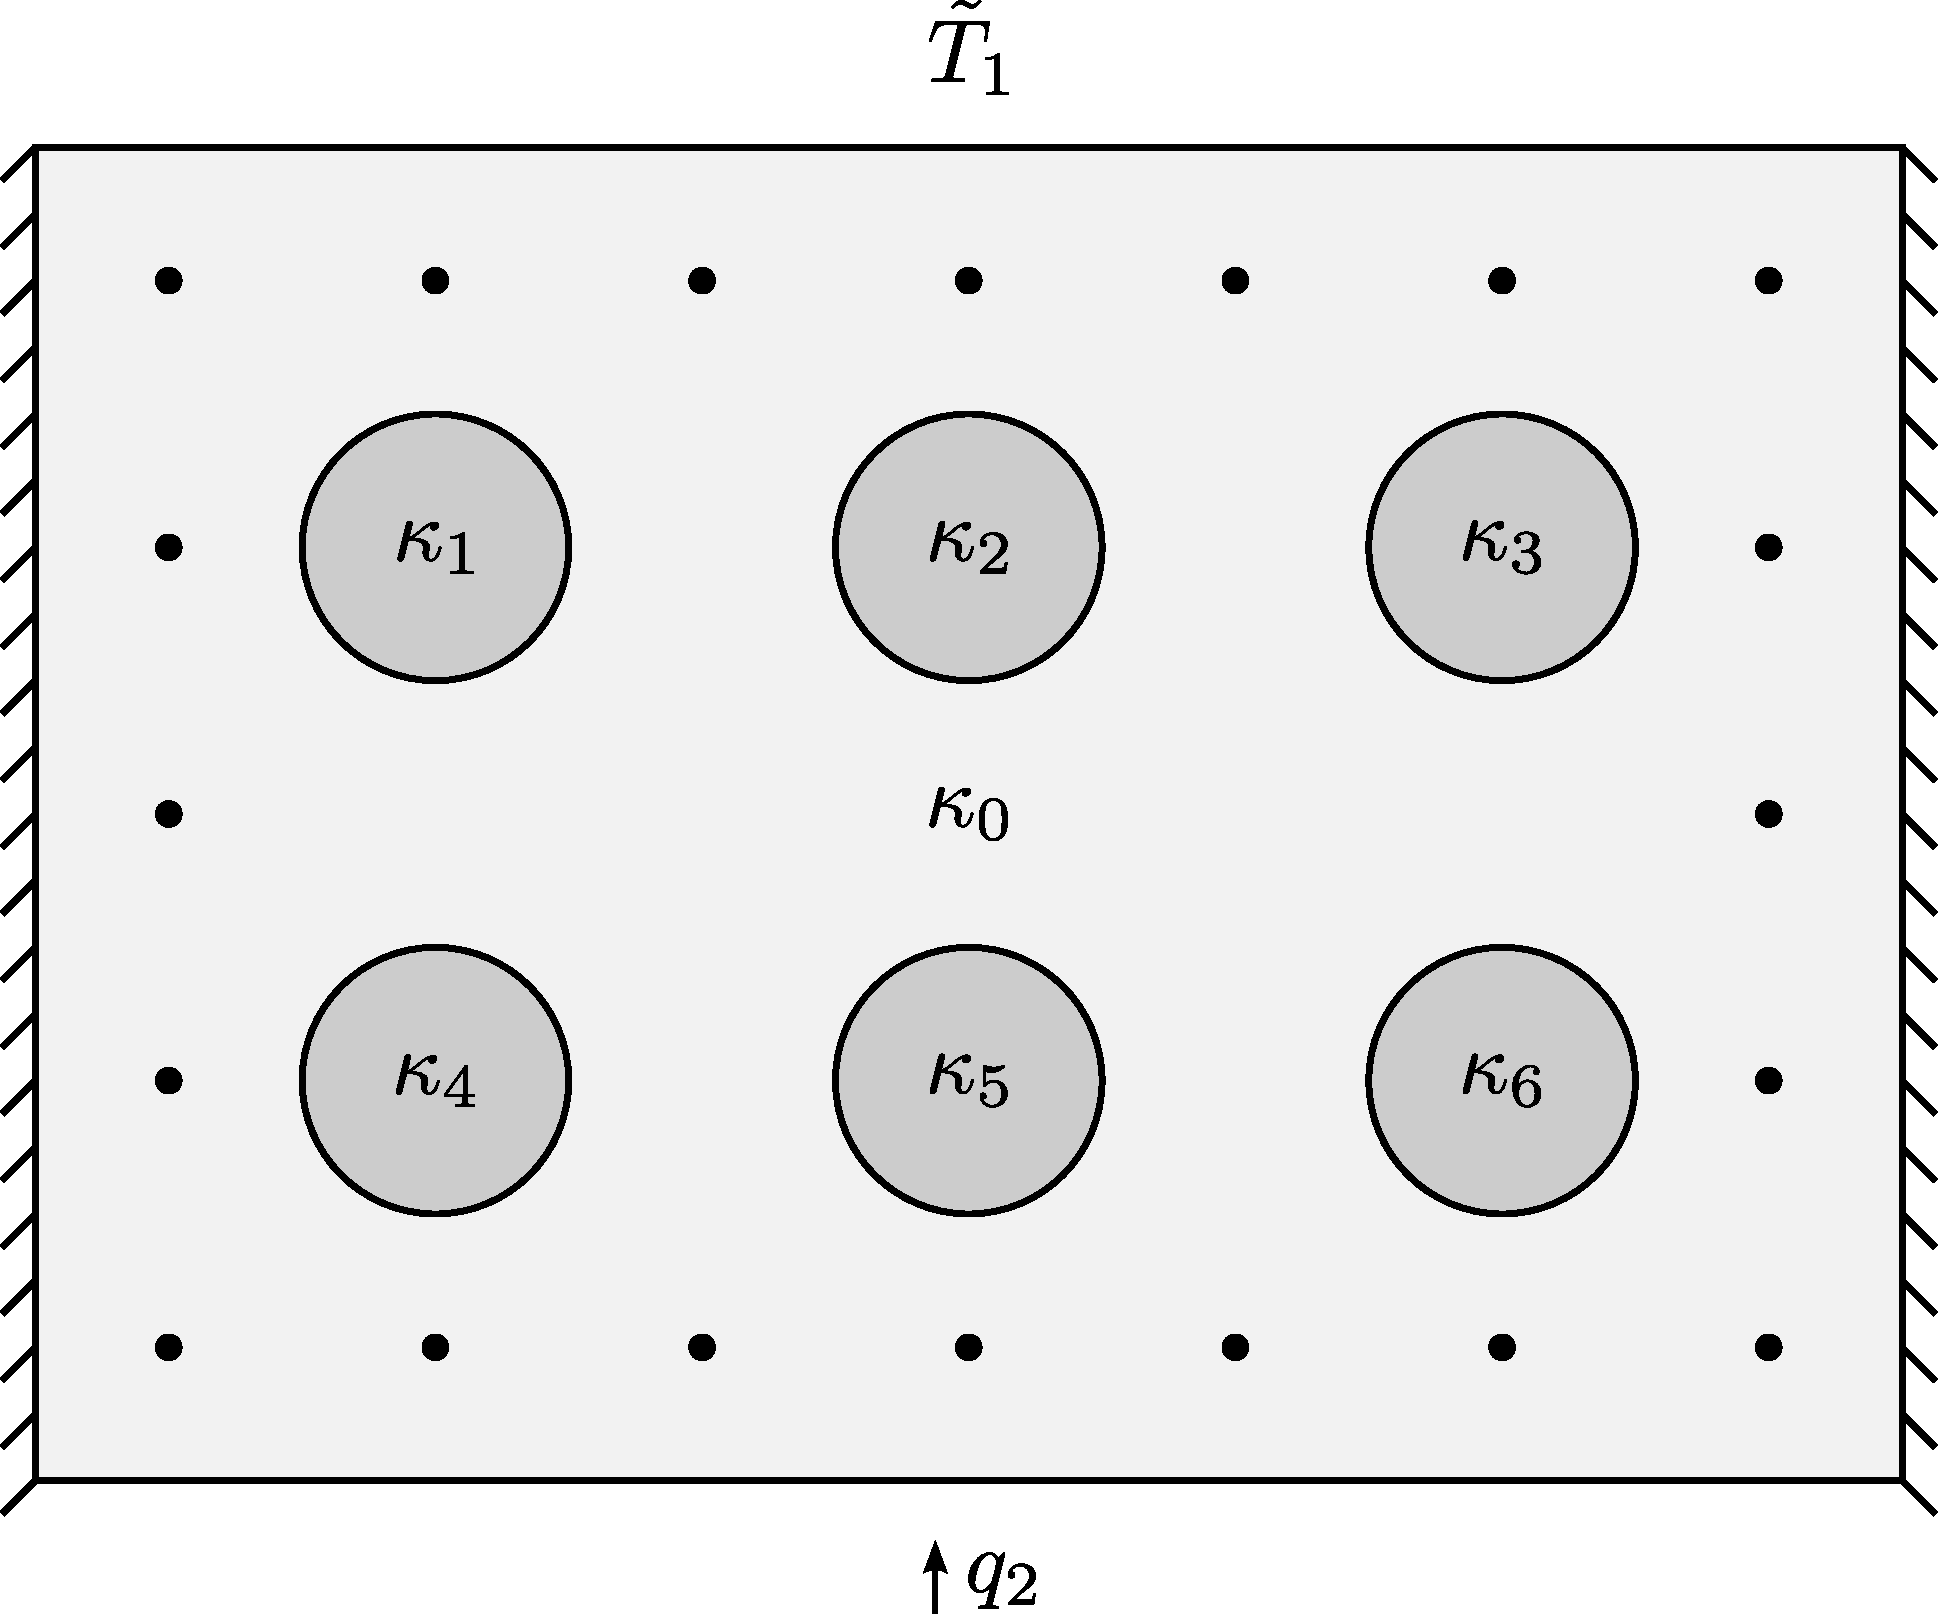
\includegraphics[width=\JCPfemWidth]{fig_JCP_Heat6D_HeatConduction}
  \caption[6D IHCP: Heat conduction setup]{6D IHCP: Heat conduction setup.}
  \label{fig:JCP:Thermal:HeatConduction}
\end{figure}

\subsubsection{Posterior density}
% LIKELIHOOD EXPANSION
The unknowns are represented as \(\kappa_i = \exp(\lambda_0 + \varsigma_0 \xi_i)\) in terms of the standardized variables
\(\xi_i \in \mathds{R}\) with Gaussian weight functions \(\mathcal{N}(\xi_i \cond 0,1)\).
A spectral expansion \(\hat{\mathcal{L}}_p\) in tensorized Hermite polynomials is then computed for \(p = 5\) and \(K = 5 \times 10^4\).
The errors of the likelihood approximation are estimated as \(\epsilon_{\mathrm{Emp}} = 8.81 \times 10^{-1}\) and \(\epsilon_{\mathrm{LOO}} = 9.14 \times 10^{-1}\).
As compared to the low-dimensional examples that were studied before, these are large errors.
% BASELINE CHANGE
An auxiliary reference density \(\newBase(\bm{\kappa}) = \prod_{i=1}^6 \newBase(\kappa_i)\) is then constructed as a
multivariate lognormal with independent marginals \(\newBase(\kappa_i) = \mathcal{LN}(\kappa_i \cond \mu_i,\sigma_i^2)\).
The parameters of the latter are chosen as the means \(\mu_i = \mathds{E}[\kappa_i \cond \bm{T}]\) and standard deviations
\(\sigma_i = \mathrm{Std}[\kappa_i \cond \bm{T}]\) of the posterior surrogate corresponding to the coefficients of SLE \(\hat{\mathcal{L}}_p\).
We remark that this is a simple two-step procedure and that a more refined usage of the reference change would certainly lead to more sophisticated approaches.
Subsequently, an aSLE \(\hat{\auxQuantity}_p\) with \(p = 5\) and  \(K = 5 \times 10^4\) is computed.
The errors amount to \(\epsilon_{\mathrm{Emp}} = 4.81 \times 10^{-1}\) and \(\epsilon_{\mathrm{LOO}} = 6.24 \times 10^{-1}\).
Notwithstanding that these errors are smaller than the corresponding errors of the SLE, they are still large as compared to the previous examples.
Since these errors are now measured with respect to the auxiliary density which is expectedly closer to the true posterior than the prior is,
the aSLE presumably leads to a more accurate posterior surrogate.
\par % 1D MARGINALS
From the previously computed SLE \(\hat{\mathcal{L}}(\bm{\kappa})\) and the aSLE \(\hat{\auxQuantity}_p(\bm{\kappa})\)
approximations of the joint posterior density are computed via \cref{eq:JCP:SLE:Posterior,eq:JCP:SLE:BaselineChange:Posterior}.
The obtained surrogates \(\pi(\bm{\kappa} \cond \bm{T}) \approx \hat{\mathcal{L}}_p(\bm{\kappa}) \pi(\bm{\kappa}) / \coeffL_{\bm{0}}\) and
\(\pi(\bm{\kappa} \cond \bm{T}) \approx \hat{\auxQuantity}_p(\bm{\kappa}) \newBase(\bm{\kappa}) / \coeffBaseL_{\bm{0}}\) are now compared to each other.
We start with the one-dimensional marginals that can be compiled by collecting terms from the full expansions based on \cref{eq:JCP:SLE:Marginal1D}.
For \(j = 1,\ldots,6\) the marginals \(\pi(\kappa_j \cond \bm{T})\) that are extracted that way are shown in \cref{fig:JCP:Thermal:Post1D}.
The marginal priors \(\pi(\kappa_j)\) and the auxiliary densities \(\newBase(\kappa_j)\) are shown, too.
% DISCUSSION
While the marginals that are taken from the SLE slightly deviate from their MCMC counterparts, the marginals based on the aSLE match their references perfectly well.
The reason is that the posterior can be easier represented as a small adjustment of the auxiliary density than as a large correction to the prior.
Thus, with the same expansion order the posterior is more accurately represented through the aSLE than through the SLE.
Regarding the size of the error estimates, it is surprising that the marginals can be retrieved that well with the aSLE.
Even though the SLE-based posterior approximations can hardly be interpreted as proper probability densities, i.e.\ they conspicuously take on negative values,
the moments are recovered sufficiently well for the construction of the auxiliary reference density.
% POSTERIOR MARGINALS
\begin{figure}[htbp]
  \centering
  \begin{subfigure}[b]{\JCPsubWidth}
    \centering
    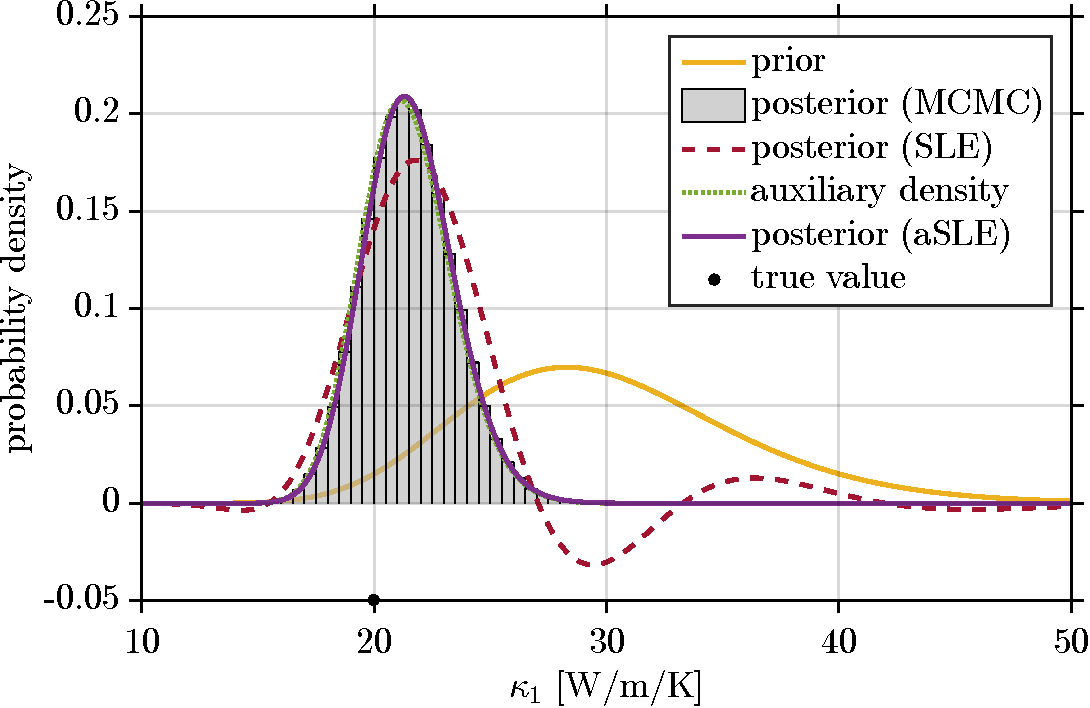
\includegraphics[height=\JCPfigHeight]{fig_JCP_Heat6D_Post1D_k1}
    \caption{Thermal conductivity \(\kappa_1\).}
    \label{fig:JCP:Thermal:Post1D:k1}
  \end{subfigure}\hfill%
  \begin{subfigure}[b]{\JCPsubWidth}
    \centering
    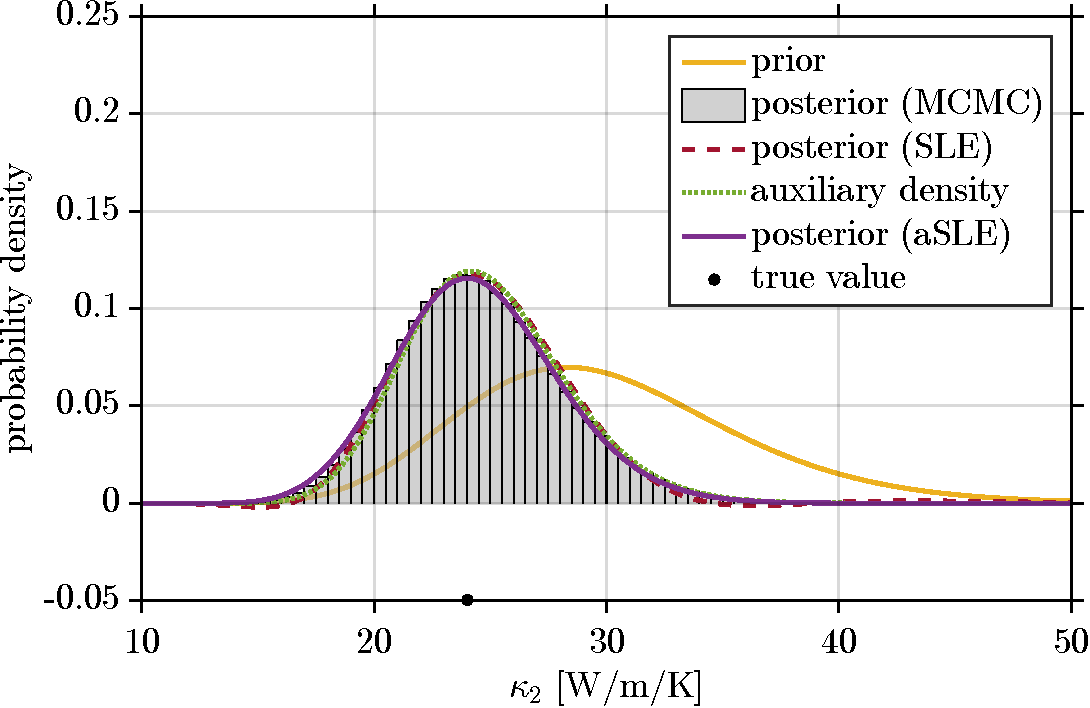
\includegraphics[height=\JCPfigHeight]{fig_JCP_Heat6D_Post1D_k2}
    \caption{Thermal conductivity \(\kappa_2\).}
    \label{fig:JCP:Thermal:Post1D:k2}
  \end{subfigure}\\[3ex]%
  \begin{subfigure}[b]{\JCPsubWidth}
    \centering
    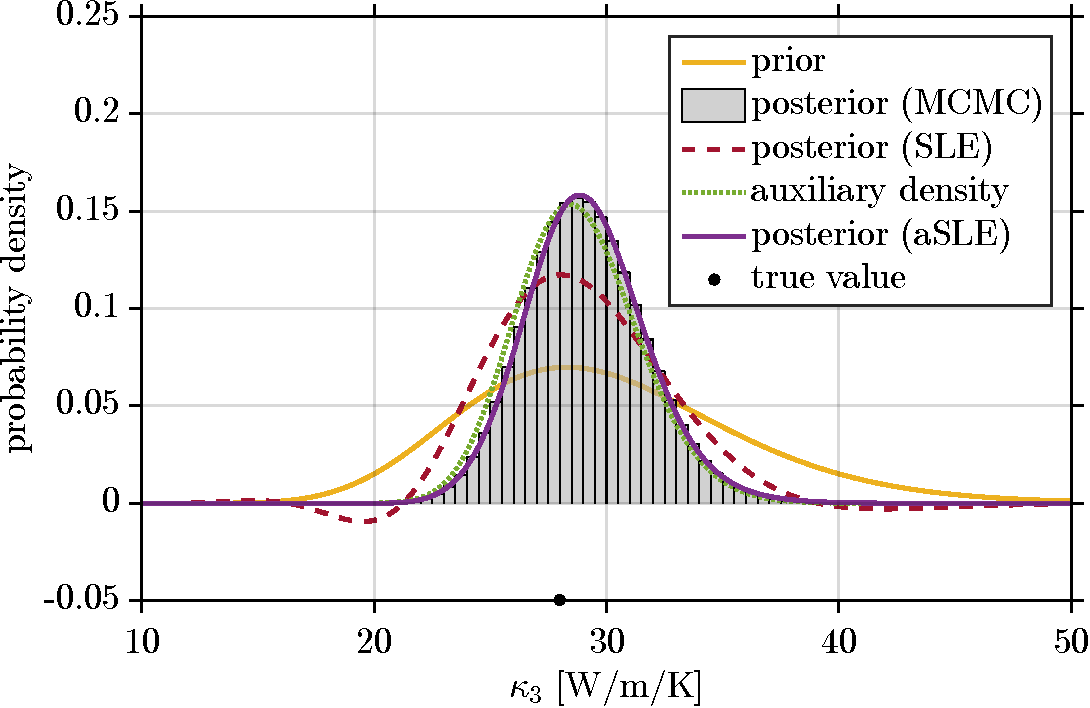
\includegraphics[height=\JCPfigHeight]{fig_JCP_Heat6D_Post1D_k3}
    \caption{Thermal conductivity \(\kappa_3\).}
    \label{fig:JCP:Thermal:Post1D:k3}
  \end{subfigure}\hfill%
  \begin{subfigure}[b]{\JCPsubWidth}
    \centering
    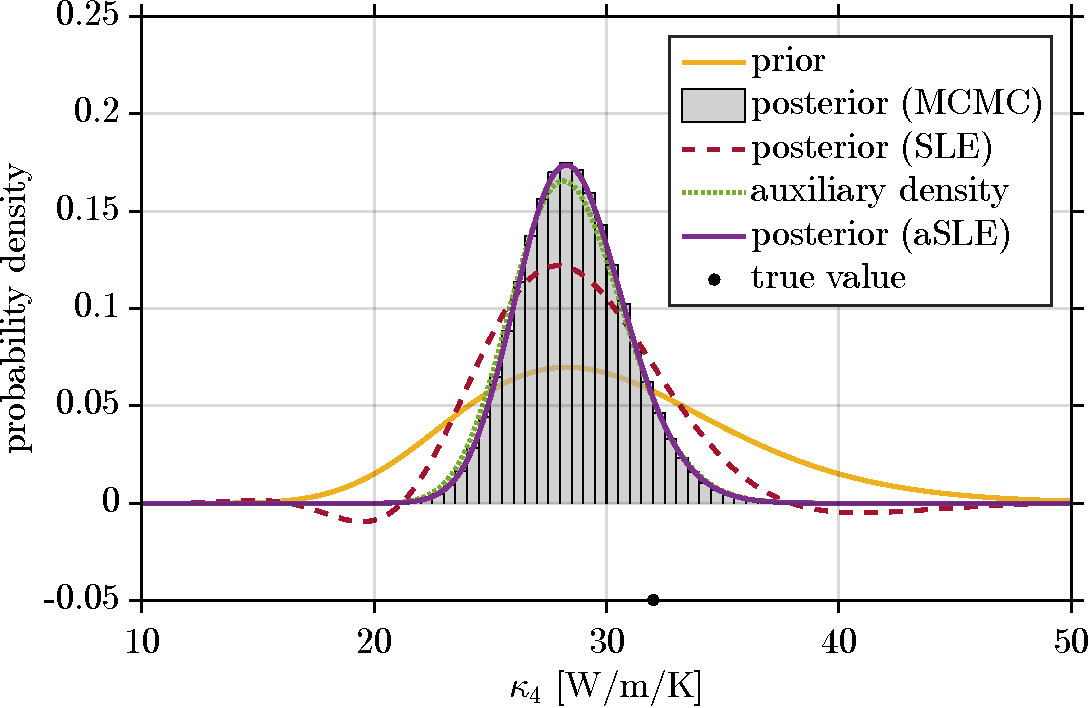
\includegraphics[height=\JCPfigHeight]{fig_JCP_Heat6D_Post1D_k4}
    \caption{Thermal conductivity \(\kappa_4\).}
    \label{fig:JCP:Thermal:Post1D:k4}
  \end{subfigure}\\[3ex]%
  \begin{subfigure}[b]{\JCPsubWidth}
    \centering
    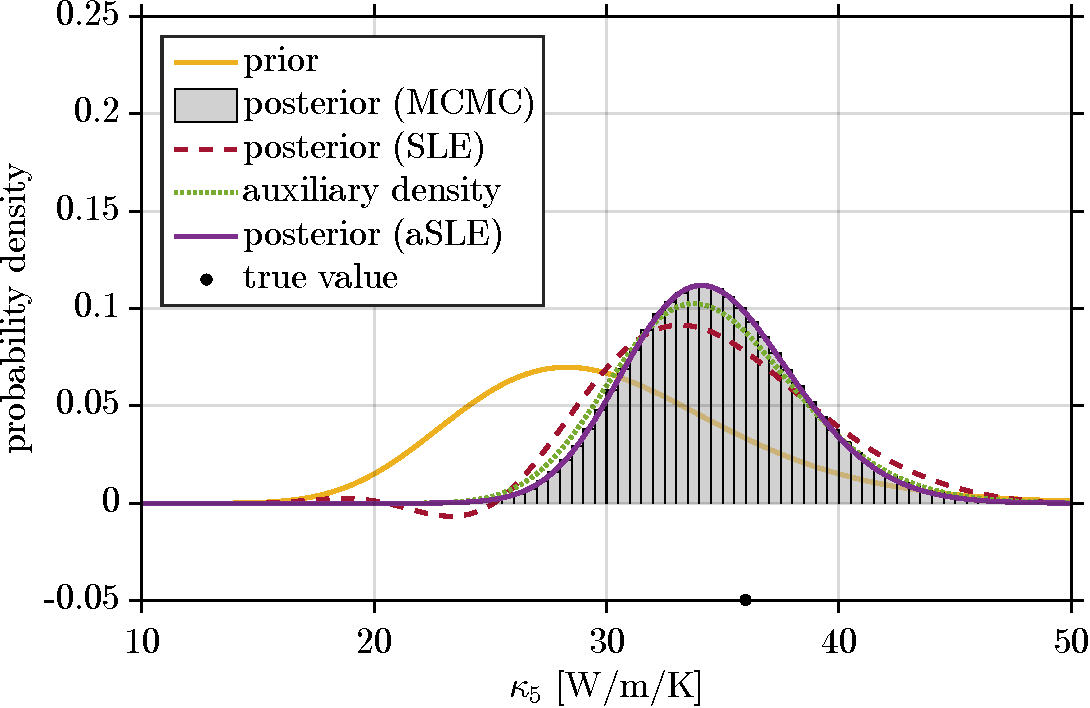
\includegraphics[height=\JCPfigHeight]{fig_JCP_Heat6D_Post1D_k5}
    \caption{Thermal conductivity \(\kappa_5\).}
    \label{fig:JCP:Thermal:Post1D:k5}
  \end{subfigure}\hfill%
  \begin{subfigure}[b]{\JCPsubWidth}
    \centering
    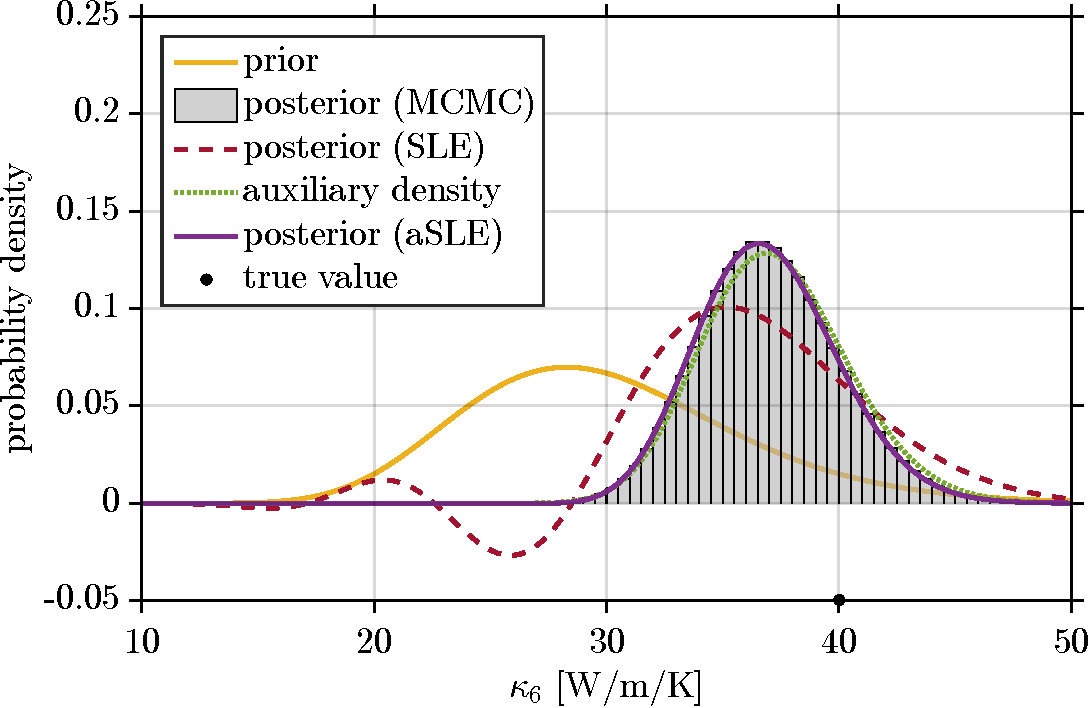
\includegraphics[height=\JCPfigHeight]{fig_JCP_Heat6D_Post1D_k6}
    \caption{Thermal conductivity \(\kappa_6\).}
    \label{fig:JCP:Thermal:Post1D:k6}
  \end{subfigure}%
  \caption[6D IHCP: Posterior marginals]{6D IHCP: Posterior marginals.}
  \label{fig:JCP:Thermal:Post1D}
\end{figure}
\par % 2D MARGINALS
On the basis of \cref{eq:JCP:SLE:Marginal2D} the two-dimensional posterior marginals \(\pi(\kappa_j,\kappa_k \cond \bm{T})\) can be constructed from the full expansions.
For \(j = 3\) and \(k = 4\) the posterior marginal for the SLE \(\hat{\mathcal{L}}_p\) is shown in \cref{fig:JCP:Thermal:Post2D:SLE}.
The same two-dimensional distribution is depicted in \cref{fig:JCP:Thermal:Post2D:aSLE} for the aSLE \(\hat{\auxQuantity}_p\).
A histogram of the MCMC sample is provided in \cref{fig:JCP:Thermal:Post2D:MCMC} as a reference.
As already found in \cref{fig:JCP:Thermal:Post1D:k3,fig:JCP:Thermal:Post1D:k4} for instance,
in \cref{fig:JCP:Thermal:Post2D} the aSLE-based surrogate appears to be almost exact whereas the SLE-based one is flattened out.
Since the aSLE captures the true posterior density more accurately than the SLE, we expect similar findings for the posterior moments.
% FIGURES: 2D POSTERIORS
\begin{figure}[htbp]
  \centering
  \begin{subfigure}[b]{\JCPsubWidth}
    \centering
    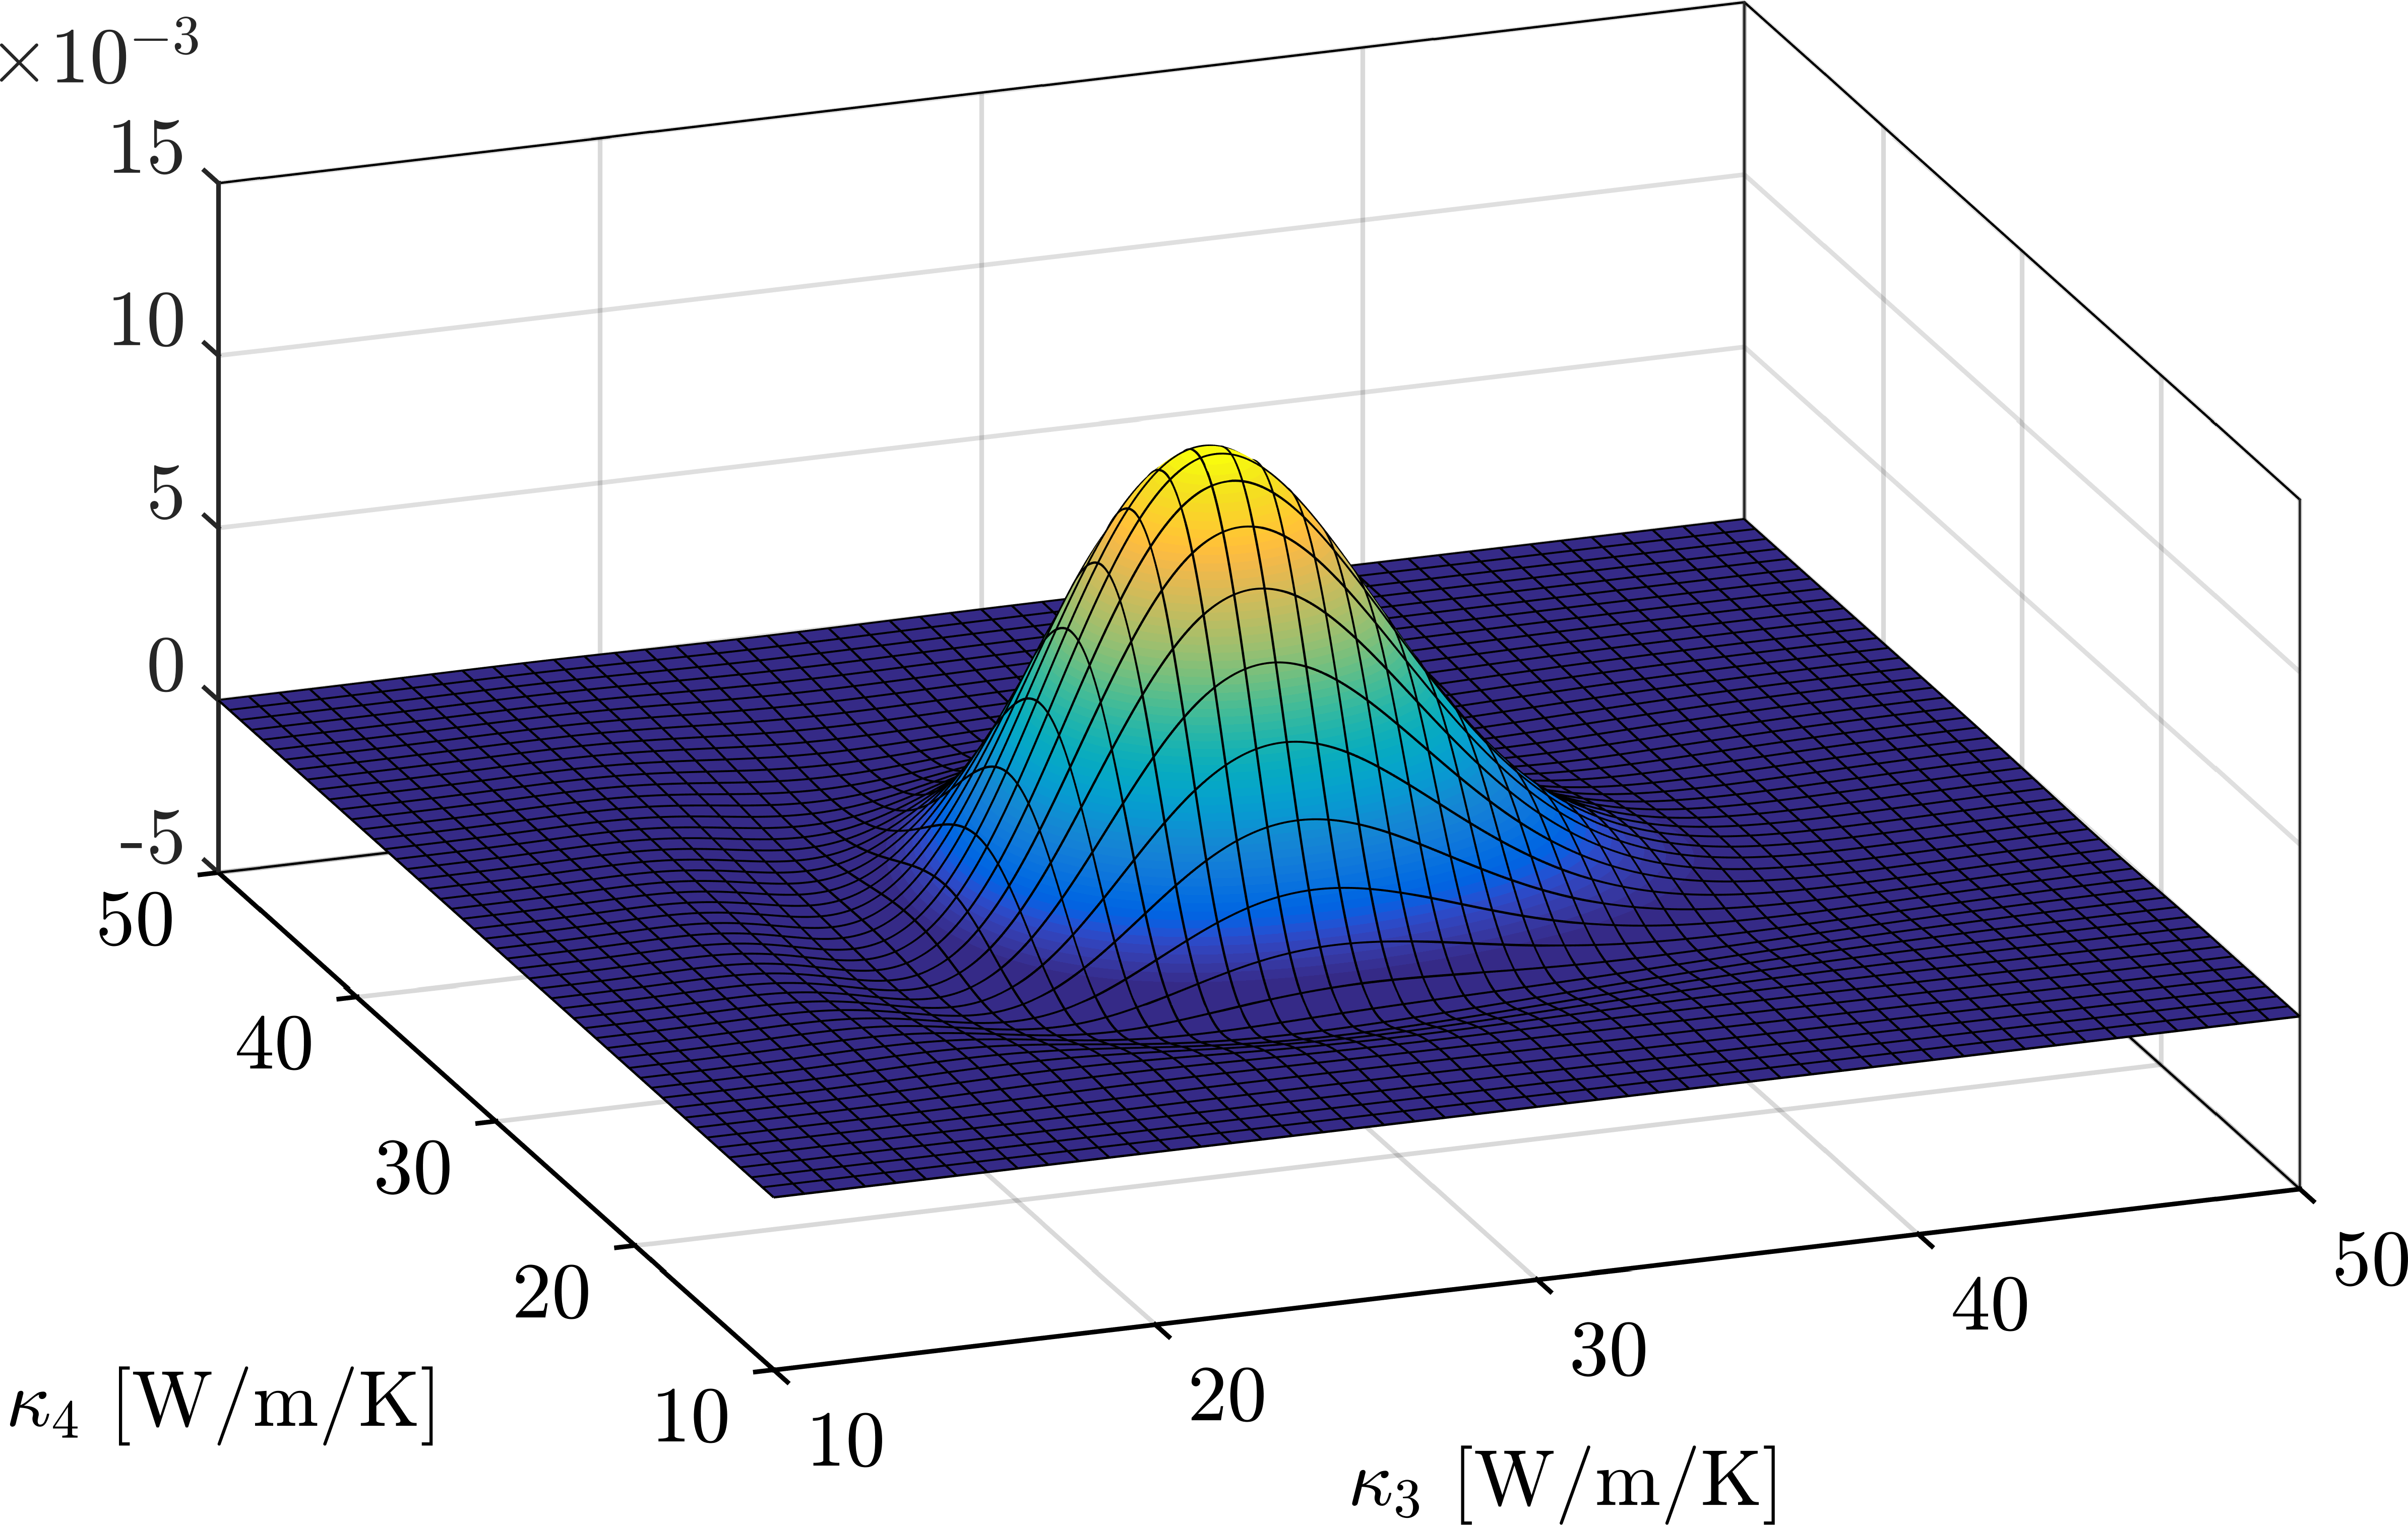
\includegraphics[width=\JCPfigWidth]{fig_JCP_Heat6D_Post2D_SLE}
    \caption{SLE with \(p = 5\).}
    \label{fig:JCP:Thermal:Post2D:SLE}
  \end{subfigure}\hfill%
  \begin{subfigure}[b]{\JCPsubWidth}
    \centering
    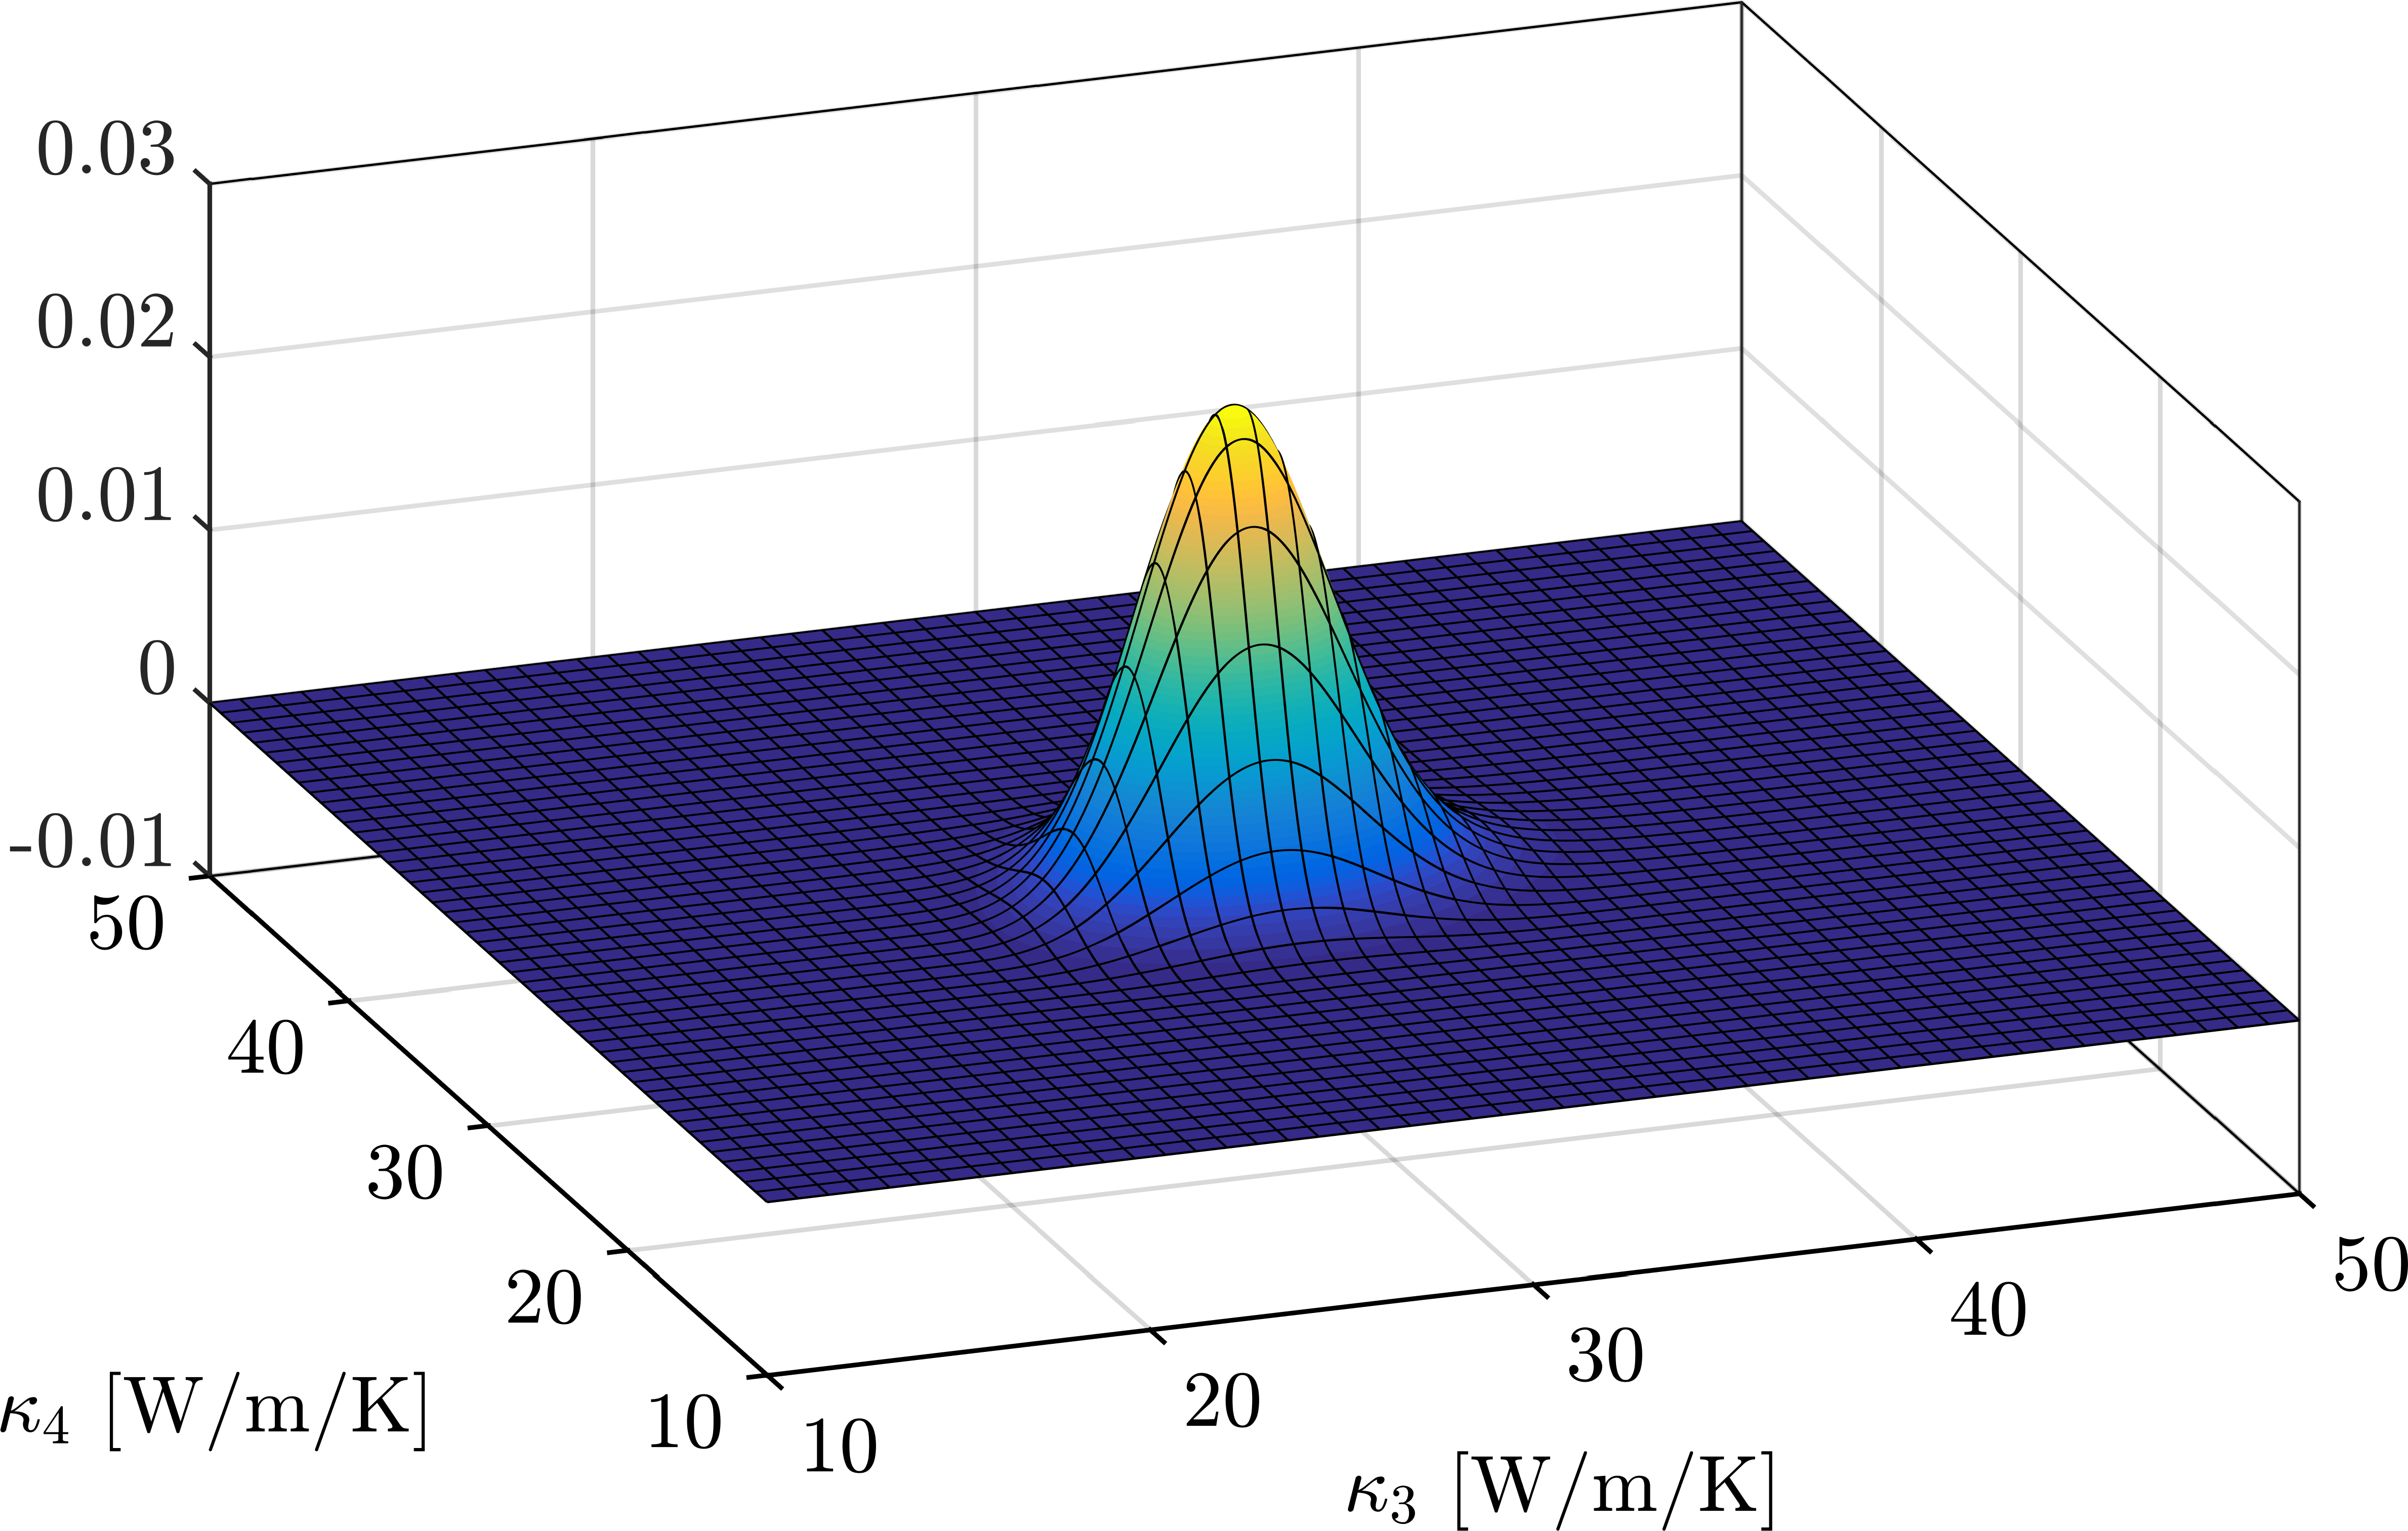
\includegraphics[width=\JCPfigWidth]{fig_JCP_Heat6D_Post2D_aSLE}
    \caption{aSLE with \(p = 5\).}
    \label{fig:JCP:Thermal:Post2D:aSLE}
  \end{subfigure}\\[1ex]%
  \begin{subfigure}[b]{\JCPsubWidth}
    \centering
    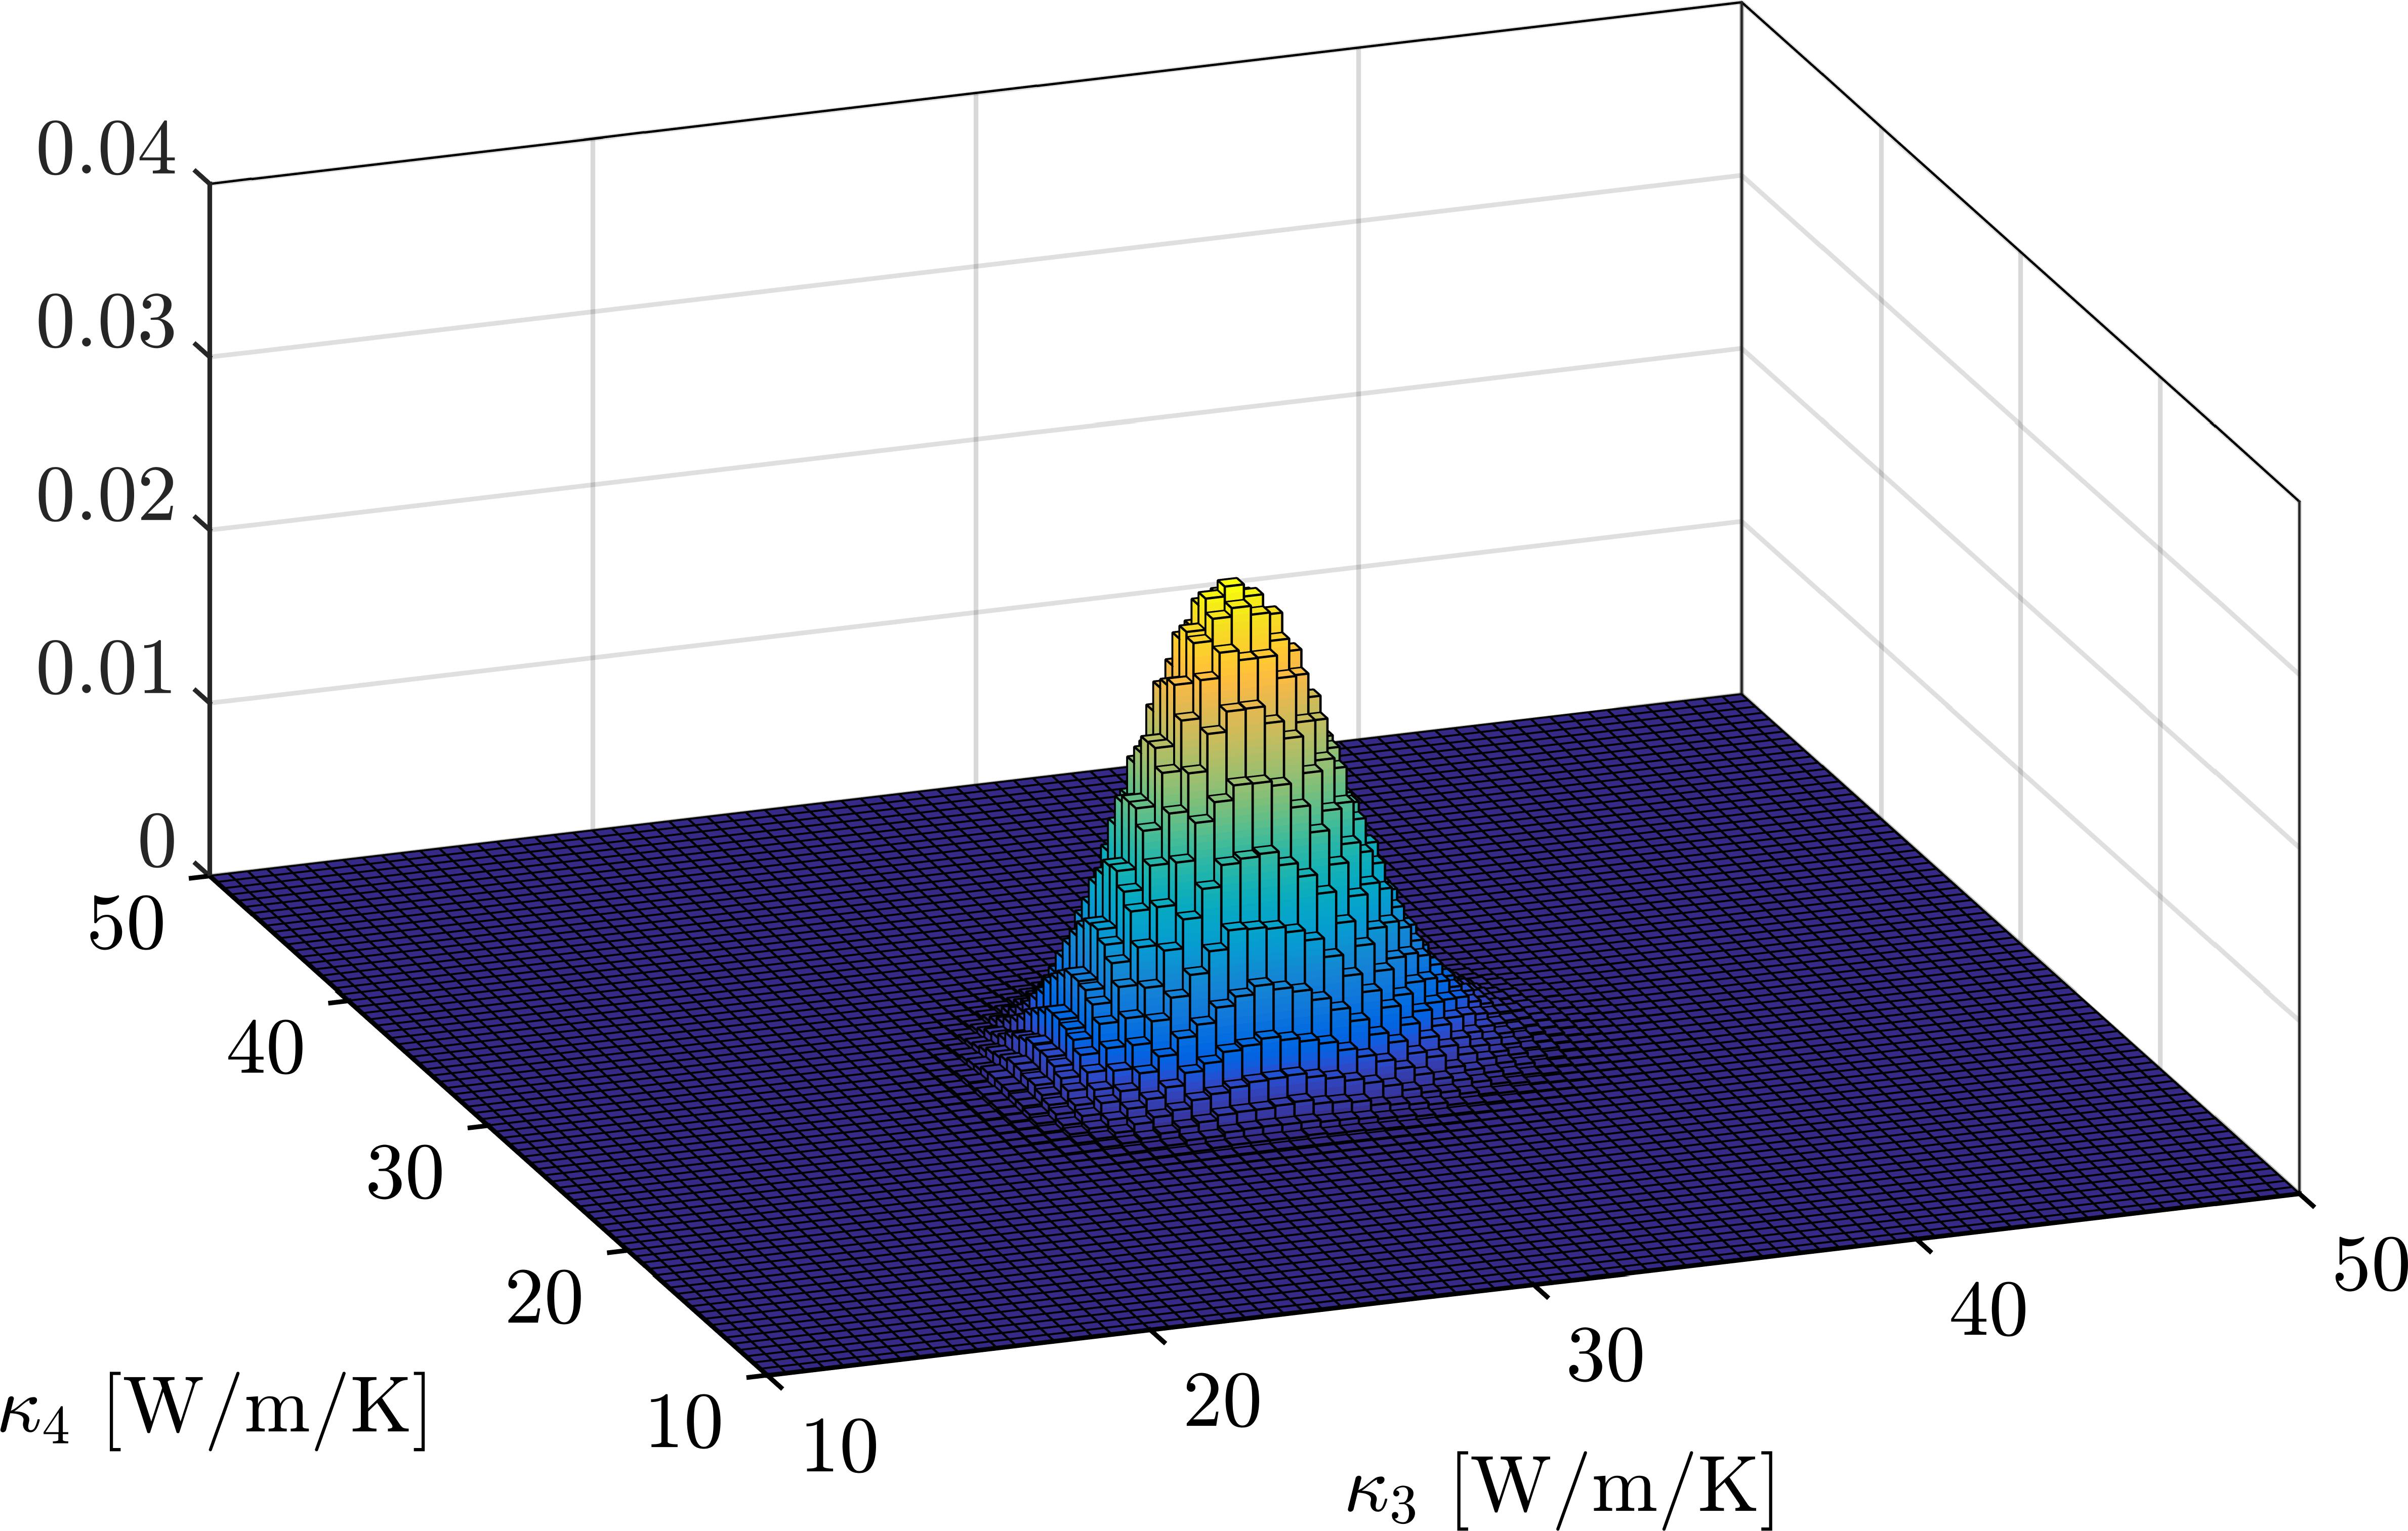
\includegraphics[width=\JCPfigWidth]{fig_JCP_Heat6D_Post2D_MCMC}
    \caption{MCMC reference sample.}
    \label{fig:JCP:Thermal:Post2D:MCMC}
  \end{subfigure}%
  \caption[6D IHCP: Posterior marginals]{6D IHCP: Posterior marginals.}
  \label{fig:JCP:Thermal:Post2D}
\end{figure}

\subsubsection{Quantities of interest}
% STATISTICAL QUANTITIES OF INTEREST
Finally we compute the model evidence and the first posterior moments with the aid of
\cref{eq:JCP:SLE:ScaleFactor,eq:JCP:SLE:BaselineChange:ScaleFactor} and \cref{eq:JCP:SLE:PosteriorMargMean,eq:JCP:SLE:PosteriorMargVariance,eq:JCP:SLE:PosteriorCovariance}.
For the aSLE \(\hat{\auxQuantity}_p\) the analysis proceeds analogously to the SLE \(\hat{\mathcal{L}}_p\).
In \cref{tab:JCP:Thermal:StatisticalQuantities} a summary of the results is given.
As it can be taken from the table, the aSLE consistently gives more accurate estimates of the reference values.
This fulfills our earlier expectations.
Regarding the inaccuracy of the SLE-based posterior marginals and the concerns about interpreting them as probability densities, 
the quality of the SLE-based estimates of the moments surpasses our expectations.
In particular, the estimated standard deviations are more accurate than the surrogate marginals suggest, e.g.\ the ones shown in \cref{fig:JCP:Thermal:Post1D:k1,fig:JCP:Thermal:Post1D:k6}.
Similar as for the posterior density, we have to conclude that the normalized LOO error does not give conclusive information about the accuracy of the first posterior moments.
Nevertheless, it is remarked that the use of resampling methods still ensures a robust fit, i.e.\ it protects against overfitting.
% TABLE: STATISTICAL QUANTITIES
\begin{table}[htbp]
  \caption[6D IHCP: Statistical quantities]{6D IHCP: Statistical quantities.}
  \label{tab:JCP:Thermal:StatisticalQuantities}
  \centering
  \begin{tabular}{rccccccc}
    \toprule
    & \(\scale\) \([10^{-3}]\) & \(\mathds{E}[\kappa_1 \cond \bm{T}]\) & \(\mathds{E}[\kappa_2 \cond \bm{T}]\) & \(\mathds{E}[\kappa_3 \cond \bm{T}]\)
    & \(\mathds{E}[\kappa_4 \cond \bm{T}]\) & \(\mathds{E}[\kappa_5 \cond \bm{T}]\) & \(\mathds{E}[\kappa_6 \cond \bm{T}]\) \\
    \midrule
    SLE    & \(4.04\) & \(21.42\) & \(24.86\) & \(28.79\) & \(28.45\) & \(34.43\) & \(37.27\) \\
    aSLE   & \(3.68\) & \(21.53\) & \(24.48\) & \(29.16\) & \(28.57\) & \(34.59\) & \(36.95\) \\
    (MC)MC & \(3.65\) & \(21.52\) & \(24.57\) & \(29.11\) & \(28.56\) & \(34.64\) & \(37.00\) \\
    \midrule
    & \(\mathrm{Std}[\kappa_1 \cond \bm{T}]\) & \(\mathrm{Std}[\kappa_2 \cond \bm{T}]\) & \(\mathrm{Std}[\kappa_3 \cond \bm{T}]\) & \(\mathrm{Std}[\kappa_4 \cond \bm{T}]\)
    & \(\mathrm{Std}[\kappa_5 \cond \bm{T}]\) & \(\mathrm{Std}[\kappa_6 \cond \bm{T}]\) & \(\rho[\kappa_1,\kappa_2 \cond \bm{T}]\) \\
    \midrule
    SLE    & \(1.95\) & \(3.43\) & \(2.63\) & \(2.43\) & \(3.96\) & \(3.13\) & \(-0.40\) \\
    aSLE   & \(1.94\) & \(3.56\) & \(2.61\) & \(2.33\) & \(3.62\) & \(2.99\) & \(-0.44\) \\
    (MC)MC & \(1.93\) & \(3.48\) & \(2.56\) & \(2.31\) & \(3.64\) & \(3.00\) & \(-0.47\) \\
    \midrule
    & \(\rho[\kappa_1,\kappa_3 \cond \bm{T}]\) & \(\rho[\kappa_1,\kappa_4 \cond \bm{T}]\) & \(\rho[\kappa_1,\kappa_5 \cond \bm{T}]\) & \(\rho[\kappa_1,\kappa_6 \cond \bm{T}]\)
    & \(\rho[\kappa_2,\kappa_3 \cond \bm{T}]\) & \(\rho[\kappa_2,\kappa_4 \cond \bm{T}]\) & \(\rho[\kappa_2,\kappa_5 \cond \bm{T}]\) \\
    \midrule
    SLE    & \(\hphantom{-}0.19\) & \(-0.39\) & \(-0.28\) & \(0.05\) & \(-0.40\) & \(-0.18\) & \(-0.30\) \\ 
    aSLE   & \(-0.01\) & \(-0.29\) & \(-0.03\) & \(0.10\) & \(-0.48\) & \(-0.17\) & \(-0.28\) \\
    (MC)MC & \(-0.02\) & \(-0.32\) & \(-0.03\) & \(0.09\) & \(-0.48\) & \(-0.17\) & \(-0.31\) \\
    \midrule
    & \(\rho[\kappa_2,\kappa_6 \cond \bm{T}]\) & \(\rho[\kappa_3,\kappa_4 \cond \bm{T}]\) & \(\rho[\kappa_3,\kappa_5 \cond \bm{T}]\) & \(\rho[\kappa_3,\kappa_6 \cond \bm{T}]\)
    & \(\rho[\kappa_4,\kappa_5 \cond \bm{T}]\) & \(\rho[\kappa_4,\kappa_6 \cond \bm{T}]\) & \(\rho[\kappa_5,\kappa_6 \cond \bm{T}]\) \\
    \midrule
    SLE    & \(-0.09\) & \(-0.00\) & \(\hphantom{-}0.22\) & \(-0.22\) & \(-0.20\) & \(0.24\) & \(-0.11\) \\
    aSLE   & \(-0.13\) & \(\hphantom{-}0.11\) & \(-0.02\) & \(-0.32\) & \(-0.24\) & \(0.13\) & \(-0.24\) \\
    (MC)MC & \(-0.16\) & \(\hphantom{-}0.10\) & \(-0.03\) & \(-0.34\) & \(-0.26\) & \(0.12\) & \(-0.24\) \\
    \bottomrule
  \end{tabular}
\end{table}